%% LyX 2.0.2 created this file.  For more info, see http://www.lyx.org/.
%% Do not edit unless you really know what you are doing.
\documentclass[english]{report}
\usepackage[T1]{fontenc}
\usepackage[latin9]{inputenc}
\setcounter{secnumdepth}{3}
\setcounter{tocdepth}{3}
\usepackage{float}
\usepackage{amsmath}
\usepackage{graphicx}

\makeatletter

%%%%%%%%%%%%%%%%%%%%%%%%%%%%%% LyX specific LaTeX commands.
\newcommand{\noun}[1]{\textsc{#1}}
%% Because html converters don't know tabularnewline
\providecommand{\tabularnewline}{\\}
%% A simple dot to overcome graphicx limitations
\newcommand{\lyxdot}{.}

\floatstyle{ruled}
\newfloat{algorithm}{tbp}{loa}[chapter]
\providecommand{\algorithmname}{Algorithm}
\floatname{algorithm}{\protect\algorithmname}

\makeatother

\usepackage{babel}
\begin{document}
\cleardoublepage{}


\chapter{Discovery of Object Properties}


\section{Introduction}

The previous chapters dealt with the task of a robot learning to recognise
a new object and determining its 3D shape. However, to effectively
manipulate and use an object, knowing the shape and appearance is
not always sufficient. The robot needs an internal model of the object
which, in addition to encapsulating the visual appearance and shape
of the object, also encapsulates other physical properties. Examples
of physical properties include the coefficient of friction of the
object's surface, the centre of mass and the weight of the object,
whether the object is rigid or articulated, etc. Having an accurate
model of such properties can allow the robot to effectively manipulate
and use the object to accomplish a task.

In order to determine some physical properties, passive observation
with a robot's sensors (such as a camera) may not be possible. Instead,
we present an approach in which the robot performs some actions on
an object, and the outcome of these interactions provides information
as to the underlying physical properties. 

An example of this is determining the centre of mass of a given object.
The centre of mass is dependent on the internal composition of the
object and cannot be determined by a robot through vision alone. Instead
the robot can take the object and drop it onto a flat surface from
various orientations. The resulting orientation of the object, after
each drop, provides the robot with information about the location
of the centre of mass of the object. Some of the challenges involved
include extracting from the orientation of the object information
about the location of its centre of mass, and choosing drop orientations
which provide the most information possible.

Our approach to this problem involves using a physics simulator to
generate hypotheses about the object's properties and predictions
of the outcome of a given action on a simulated model of the object.
We can then match the outcome of a real world action to the simulated
outcomes in order to determine which hypothesis model most accurately
describes the real world object. The simulated outcomes can also be
used to determine the most informative action to be performed, minimising
the total number of actions the robot needs to perform to reliably
determine the object's physical properties. Figure \ref{fig:The-experiment-loop}
shows a simple representation of the hypothesise-simulate-perform
loop of our approach. The end result is a simulated model which accurately
describes and encapsulates the physical properties of the real world
object. This simulated model can then be used to applications such
as predicting the outcome of an action on the object or planning of
tool use tasks using the object.

In this chapter we present a description of our generally applicable
approach (Section \ref{sec:Active-Robot-Learning}), followed by presenting
several concrete experiments in which the robot learns the physical
properties of an object by performing various actions (Section \ref{sec:Learning-System-Implementations}).
Next we demonstrate a tool use task in which the robot uses the learned
physical properties to plan and accomplish a set goal (Section \ref{sec:Learned-Model-Exploitation}).
Finally the chapter concludes with a discussion of the results (Section
\ref{sec:Discussion-1}), and possible avenues for future work (Section
\ref{sec:Future-Work-1}).

\begin{figure}
\begin{centering}
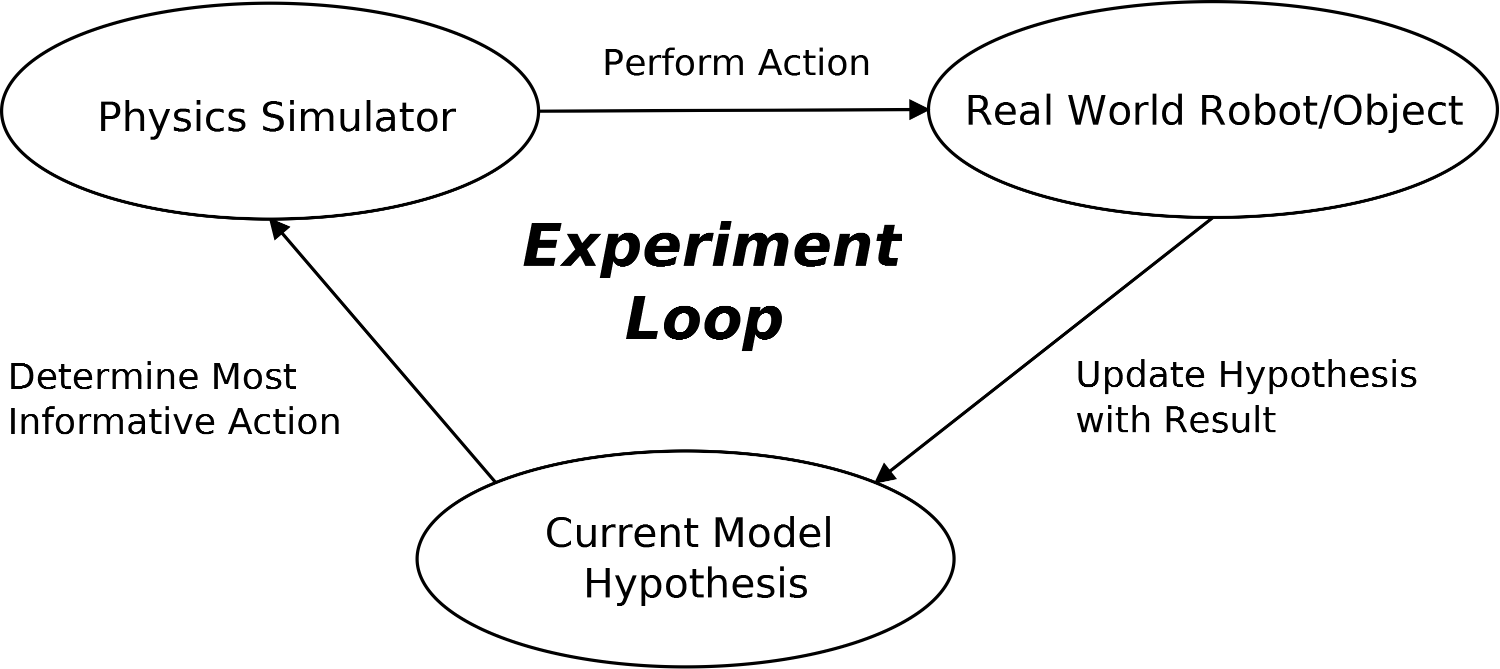
\includegraphics[width=0.7\textwidth]{images/concept}
\par\end{centering}

\caption{The experiment loop view of our system. The robot uses a physics simulator
to make hypotheses about the outcome of actions on an object and uses
this to determine the most informative action. This action is then
carried out by the robot on the real world object, the result of which
is then used to update the probability distribution over hypothesis
models. This process is repeated numerous times to determine the most
accurate model of the object.\label{fig:The-experiment-loop}}
\end{figure}



\section{Active Robot Learning Framework\label{sec:Active-Robot-Learning}}


\subsection{Problem Definition}

The problem we solve is how can a robot best determine the underlying
physical properties of an object by performing some actions and observing
the outcomes. First we specify the problem in concrete terms. Let
there be an object which the robot can recognise and localise in a
scene. The the 3D shape of this object is known. The goal is to find
a model $M$ which accurately describes the physical properties of
this object, for example centre of mass or coefficient of friction.
An example application of such a model is for planning tasks using
the object and predicting action outcomes.

Let us define the following:
\begin{itemize}
\item list of possible models $H=\left\{ h_{1},h_{2},\ldots,h_{n}\right\} $
that can describe the object;
\item discrete probability distribution $C=\left\{ c_{1},c_{2},\ldots,c_{n}\right\} \mid c_{i}=P\left(M=h_{i}\right)$
which represents the confidence of a corresponding model accurately
describing the object;
\item set of actions $A=\left\{ a_{1},a_{2},\ldots,a_{m}\right\} $ that
can be carried out by the robot;
\item set of possible action outcomes $R=\left\{ r_{1},r_{2},\ldots,r_{l}\right\} $,
where the result of each action $a\in A$ is some $r\in R$.
\end{itemize}
The goal is to determine the model $h\in H$ which most accurately
describes the object, such that $M=h$. To do this, the robot repeatedly
performs actions $a\in A$, observes the results, and updates the
confidence distribution $C$ accordingly. After several iterations,
the model $h_{x}$ with the highest corresponding confidence $c_{x}$
is taken to be the model which best describes the object ($M=h_{x}$).


\subsection{Approach Overview}

To achieve this goal, our approach is for the robot to simulate the
outcome of various actions on the various possible models, carry out
the most informative one in the real world, and update the confidence
distribution based on how the outcome compares to the simulations.
That is, robot carries out a series of actions $a\in A$, the outcome
of each is a result $r\in R$. The properties of the object affect
the outcome of a given action, therefore the result of each action
is used to perform a Bayesian update of the probability distribution
$C$. After a number of iterations the highest confidence possible
model $h$ is taken to be the model $M$ that accurately describes
the object. That is, we assign to $M$ the hypothesis model $h_{i}$
with the highest confidence at the conclusions of the experiment loop:

\begin{center}
${\displaystyle {\displaystyle M\leftarrow h_{i}\mid\forall j\neq i:c_{i}\geq c_{j}}}$
\par\end{center}

The challenges involved include: representing the object models, determining
the best actions to perform, and updating the probability distribution
over the possible models using the outcome result of a given action.
In this section we describe our general object model learning approach
which addresses these challenges. Further on in this chapter we present
some concrete implementations, demonstrating the effectiveness and
suitability of our approach to a variety of problems.

The learning algorithm consists of several distinct steps. First a
result probability model of all of the available actions is built
(described in Subsection \ref{sub:Experiment-Model}), followed by
generating a discrete set of possible result labels $R$ (described
in Subsection \ref{sub:Result-Labels}). After these initialisation
steps, the robot performs the experimentation loop. In this loop the
robot determines the most informative action based on the current
confidence distribution and action probability models (described in
Subsection \ref{sub:Choosing-an-Experiment}), performs the best action,
and finally updates the confidence distribution using the result.
After a desired number of iterations, the model with the highest confidence
is returned as the best model $M$. These steps are outlined in a
flowchart in Figure \ref{fig:Flowchart-model} and in ruther detail
in Algorithm \ref{alg:Object-Model-Learning}.

\begin{figure}
\begin{centering}
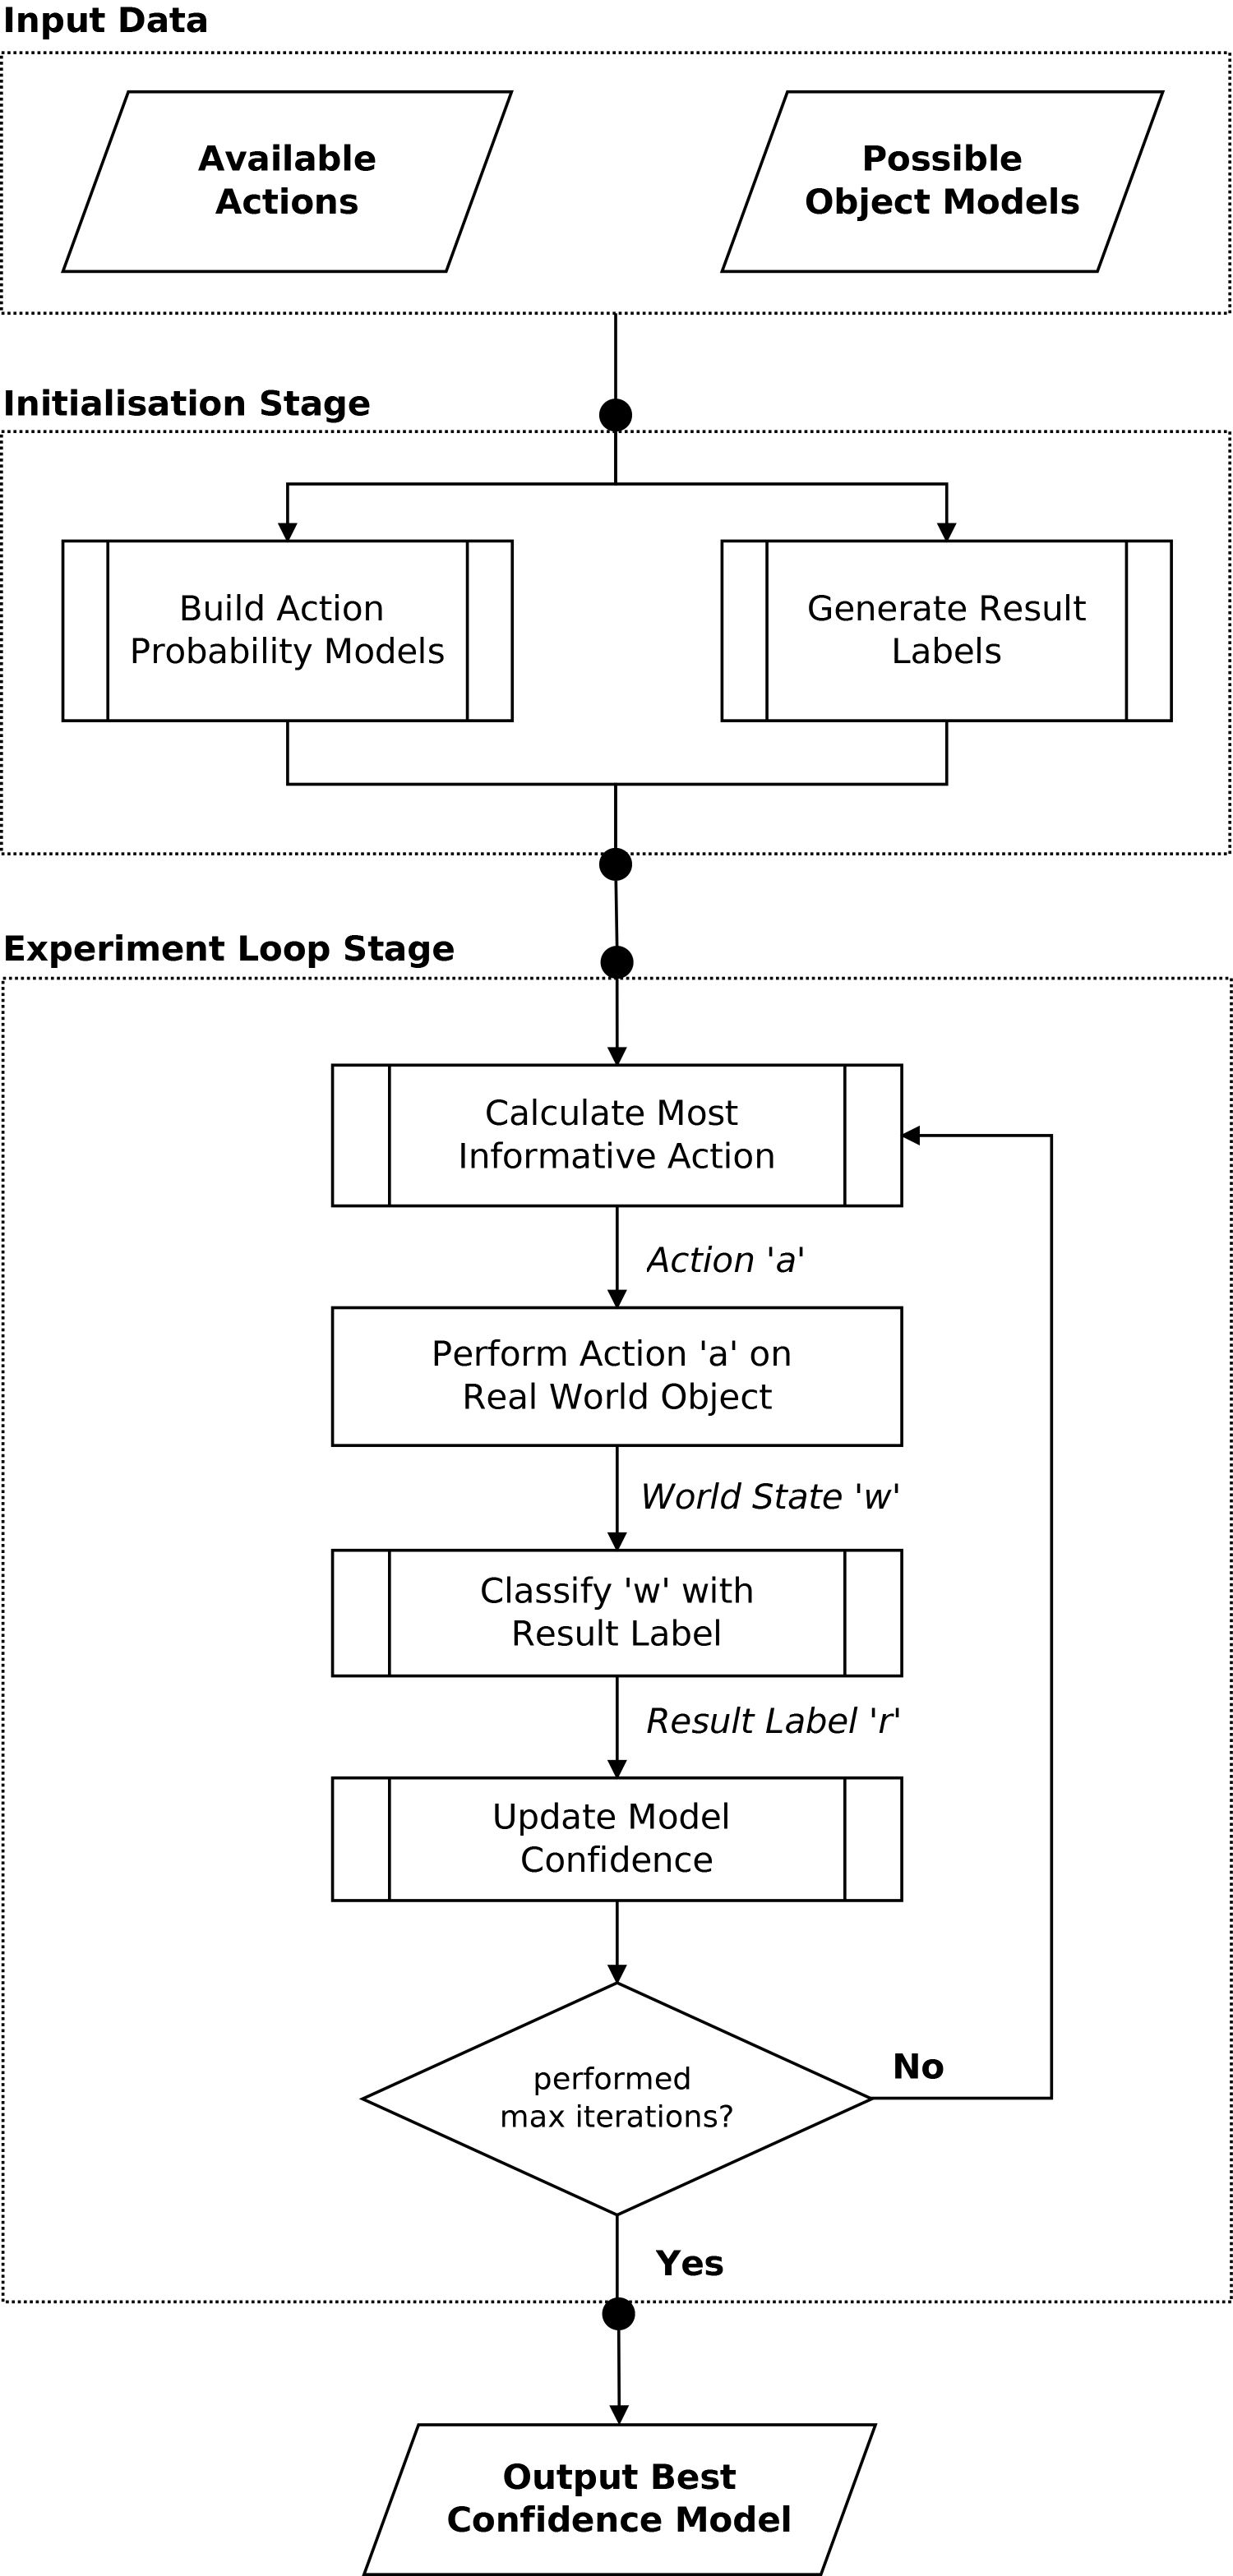
\includegraphics[width=0.7\textwidth]{images/overview}
\par\end{centering}

\caption{Flowchart representing the work-flow of the object model learning
system.\label{fig:Flowchart-model}}


\end{figure}


\begin{algorithm}
\textbf{input:} set of actions $\rightarrow A$

\textbf{input:} set of possible models $\rightarrow H$

\medskip{}


$C_{current}\leftarrow\left\{ \dfrac{1}{|H|}\right\} $

$buildActionModels(A,H)$

$R\leftarrow buildResultLabels(A,H)$

\textbf{repeat}

~~~~$a_{best}\leftarrow mostInformativeFrom(A,C_{current})$

~~~~$world\_state\leftarrow performAction(a_{best})$

~~~~$r\leftarrow classifyToResultLabel(world\_state,R)$

~~~~$C_{new}\leftarrow updateModelConfidence(C_{current},r)$

~~~~$C_{current}\leftarrow C_{new}$

\textbf{until} \emph{$max\_iterations$}

\medskip{}


$highest\_confidence\leftarrow0$

\textbf{forall} $h_{i}$ \textbf{in} $H$

~~~~\textbf{if} $c_{i}>highest\_confidence$ \textbf{then}

~~~~~~~~$highest\_confidence\leftarrow c_{i}$

~~~~~~~~$M\leftarrow h_{i}$

~~~~\textbf{endif}

\textbf{endfor}

\medskip{}


\textbf{output:} most accurate object model $\leftarrow M$

\caption{Object model learning algorithm.\label{alg:Object-Model-Learning}}


\end{algorithm}



\subsection{Object Model Representation}

The object model refers to the way in which the robot internally represents
a given object. Object model representation is one of the key aspects
of a robot system learning to interact with and use an object. A particular
model determines the different object properties that can be represented,
as well as being used to predict the result outcomes of the robot
actions. There are many different representations that can be used
for the object model, depending on the particular application domain
in which the model will be used, and the properties of the object
that need to be encapsulated in the model. The nature of the object
model representation will also affect how it can be used for planning
and prediction.

The representation can be very low level, an approach common in the
case of developmental robotics. For example a mapping between motor
input commands and the resulting optical flow of pixels in the camera
image due to the object being moved. An example of a higher level
object model representation is to learn the motion vector of an object
when it is bumped by the robot manipulator from a given direction.
However, this type of low level explicit representation would generalise
poorly to different circumstances. For example, in the case of learning
the movement vector after a bump from a given direction, if the model
is learned on a flat surface it would then perform poorly if the object
was located on a sloped surface. To overcome these limitations, our
approach uses a physics simulator to model an object.

We use a simulated entity in a 3D physics engine as the object model
representation. There are several advantage of this approach. First,
many laws of physics are implicitly represented in the simulated environment.
The robot does not need to learn from scratch concepts such as gravity
or friction. This is in contrast to developmental approaches where
the robot must explicitly learn from experience, for example, that
an object falls down when released at a height.

Second, a wide variety of object properties can be represented, depending
on the sophistication of the physics simulator used. This includes
properties such as weight, centre of mass, coefficient of friction,
hinges and axles, etc. 

Third, the physics engine environment can be used to carry out simulated
actions on an object model to build a posterior distribution over
results for each action, build hypotheses about the object's underlying
properties, and decide on which actions it should carry out in the
real world to effeciently determine an accurate model for the object.
We elaborate on this in Subsection \ref{sub:Experiment-Model}.

Finally, a learned physics engine model can be used for predicting
the outcome of an action in a wide variety of scenarios, even if the
scenario environment differs to the one in which the object model
was learned. For example, the robot may learn the centre of mass of
a box object by dropping it onto a flat surface and observing the
results. This learned model can later be used for accurately predicting
how the box will land if it is dropped onto a sloped surface. This
would not be possible if the model used was, for example, a simple
mapping from angle of release to final resting orientation of the
box.


\subsection{Action Probability Model\label{sub:Experiment-Model}}

The action probability model refers to the likelyhood of observing
a particular result when performing a given action on an object with
properties matching a specific model. 

In order to determine the model which most accurately describes the
object, the robot performs a series of actions. The specifics of each
action will depend largely on the nature of the object, the physical
properties of interest, and the methods of manipulation available
to the robot. However, the overall structure of the action probability
model and how it fits into the overall framework remains the same.

When the robot performs an action $a\in A$, the outcome is some world
state which can be labeled $r\in R$, where $R$ is a discrete and
finite set of possible results (how a result is labeled is described
in the following section). Using this outcome, we can use Bayesian
inference to update the probability distribution $C$ over the possible
models. Bayesian inference is the application of Bayes rule to calculate
the change in a belief distribution due to newly acquired evidence.
This is expressed in the following equation:

\begin{center}
${\displaystyle {\displaystyle P\left(B|E\right)=\dfrac{P\left(E|B\right)\cdot P\left(B\right)}{P\left(E\right)}}}$
\par\end{center}

where $P\left(B|E\right)$ is the posterior (the confidence of belief
$B$ being true given the new evidence $E$), $P\left(B\right)$ is
the prior (the certainty of $B$ being true before the observation
was made), $P\left(E\right)$ is the probability of observing evidence
$E$ independent of $B$, and $P\left(E|B\right)$ is the probability
of observing evidence $E$, if $B$ is known to be true. In the context
of our system, after performing action $a$ and observing result $r$,
using this formula, the robot can update the probability distribution
$C$ as follows:

\begin{center}
${\displaystyle \forall c_{i}\in C:c_{i}^{new}\leftarrow\dfrac{P\left(r|h_{i},a\right)\cdot c_{i}^{old}}{P\left(r|a\right)}}$
\par\end{center}

where $P\left(r|h_{i},a\right)$ is the probability of observing the
result $r$ when performing action $a$ on an object whose model matches
$h_{i}$, $P\left(r|a\right)$ is the probability of observing result
$r$ independent of the object model when performing action $a$,
$c_{i}^{old}$ is the prior confidence level $P\left(h_{i}\right)$,
and $c_{i}^{new}$ is the updated posterior confidence. This update
follows from the fact that the probability distribution $C$ is our
confidence that a given possible model corresponds to the object.
That is, $c_{i}^{old}=P_{prior}\left(h_{i}\right)$ and $c_{i}^{new}=P_{posterior}(h_{i}|r,a)$.

In order to perform this update, we need to know the values of the
terms $P\left(r|h_{i},a\right)$ and $P\left(r|a\right)$ for a given
action $a$. We need to calculate the probability $P\left(r|h_{i},a\right)$
of observing any given result when an action is performed on an object
described by a particular model, and the probability $P\left(r|a\right)$
of a given result when the action is performed independent of the
object's model. 

The naive method is to have the robot determine the result probabilties
by performing every action $a\in A$ on every possible object with
model $h\in H$ multiple times. However, this would be time consuming
depending on the size of $A$ and $H$. Due to the noise and errors
of manipulation and perception, each action must be performed a number
of times to determine the underlying result probability distribution.
Furthermore, this method requires the availability of a reference
object for every model $h\in H$, in order for the robot to perform
the actions on a known model. For these reasons, this approach is
not feasible.

We take an alternate approach, using the physics engine to simulate
the outcome of actions on the various possible object models. These
simulated results are used to build the probability model of each
action. This requires that each of the actions $a\in A$ can be simulated
with acceptable accuracy, such that the outcome of a simulated action
is representative of the expected outcome when performed by the robot
on the actual object. Additionally, the simulated action should account
for the errors and noise present in the system when the robot carries
out the action in the real world. We present some specific examples
of action simulation in Section \ref{sec:Learning-System-Implementations}.

Calculating the probability model for each action can be done as an
initialisation step, prior to the robot interacting with the object.
To do this each action is performed on each possible object model
in simulation. This is done multiple times such that the noise of
the action is taken into account by the probability distribution over
results. When a simulated action outputs a particular result label,
a corresponding counter is incremented for both the object model dependent
probability $P\left(r|h_{i},a\right)$ and independent probability
$P\left(r|a\right)$. At the end these counters are normalised according
to the number of simulations performed, and become the action's model
probability distributions. The process is summarised in Algorithm
\ref{alg:Calculating-the-experiment}.

\begin{algorithm}
\textbf{input:} set of actions $\rightarrow A$

\textbf{input:} set of possible models $\rightarrow H$

\textbf{input:} set of possible action results $\rightarrow R$

\medskip{}


\textbf{forall} \emph{$a$} \textbf{in} $A$

~~~~$independent\_probabilities[a]\leftarrow\{0\}$

~~~~\textbf{forall} \emph{$h$} \textbf{in} \emph{$H$}

~~~~~~~~$model\_probabilities[a][h]\leftarrow\{0\}$

~~~~~~~~\textbf{repeat}

~~~~~~~~~~~~$world\_state\leftarrow performSimulatedAction(a,h)$

~~~~~~~~~~~~$r\leftarrow classifyToResultLabel(world\_state,R)$

~~~~~~~~~~~~$independent\_probabilities[a][r]\leftarrow independent\_probabilities[a][r]+1$

~~~~~~~~~~~~$model\_probabilities[a][h][r]\leftarrow model\_probabilities[a][h][r]+1$

~~~~~~~\textbf{~until} \emph{$num\_iterations$}

\medskip{}


~~~~~~~~\textbf{forall} \emph{$x$} \textbf{in} $model\_probabilities[e][h]$

~~~~~~~~~~~~$x\leftarrow\dfrac{x}{num\_iterations}$

~~~~~~~~\textbf{endfor}

~~~~\textbf{endfor}

\medskip{}


~~~~\textbf{forall} $x$ \textbf{in} $independent\_probabilities[a]$

~~~~~~~~$x\leftarrow\dfrac{x}{|H|\cdot max\_iterations}$

~~~~\textbf{endfor}

\textbf{endfor}

\medskip{}


\textbf{output:} result probabilities $\forall a\in A:P(r|a)\leftarrow independent\_probabilities$

\textbf{output:} result probabilities $\forall a\in A,h\in H:P(r|h,a)\leftarrow model\_probabilities$

\caption{Calculating action result probabilities.\label{alg:Calculating-the-experiment}}


\end{algorithm}



\subsection{Result Labels\label{sub:Result-Labels}}

Our approach involves calculating and querying the outcome result
probability distributions $P\left(r|a\right)$ and $P\left(r|h_{i},a\right)$.
For this purpose, we represent the outcome of an action as a discrete
result label $r\in R$, were $R$ is a discrete set of all possible
outcomes. However, the world state at the conclusion of an action
is typically represented as a multi-dimensional and continuous vector
describing various aspects of the world (object pose, robot arm joints,
etc). This world state may contain a large amount of information which
is not related to the performed action and the object model. In order
to convert the world state into a result label $r$, we extract the
relevant information (for example the object pose) and match it to
a set of result bins, each of which has a corresponding label $r\in R$.
This label is the output result of an action, which can then be used
for updating the confidence distribution over possible object models,
or calculating the most informative action to perform at the current
time. 

The result bins are predefined as an initialisation step of the overall
system. The specific format of the result bins is heavily dependent
on the application domain. A simple example of generating the result
bins is by discretising the space of possible $(x,y,z)$ positions
the object may end up in after an action is carried out into uniform
cells. We then match an object pose to the closest discretised cell
and return the corresponding label. A more complex example is performing
many simulations and clustering the results using an algorithm such
as K-means in order to generate the result bins. Different methods
of generating discrete result labels are presented in detail in Section
\ref{sec:Learning-System-Implementations}.


\subsection{Choosing an Action\label{sub:Choosing-an-Experiment}}

The robot performs actions on an object and observes the results in
order to determine some underlying properties of that object. Howevere,
not all actions that the robot may perform are equally informative.
Figure \ref{fig:Good-and-bad} illustrates this concept. The worst
case scenario is if a given action gives the same result regardless
of the properties of the object. In this case the information gained
is zero. Our goal is to choose the most informative action possible
given the current level of uncertainty over the possible object models.
This reduces the number of actions that must be performed by the robot
to determine the object's properties, minimising wear and tear on
the hardware and reducing learning time. 

\begin{figure}
\begin{centering}
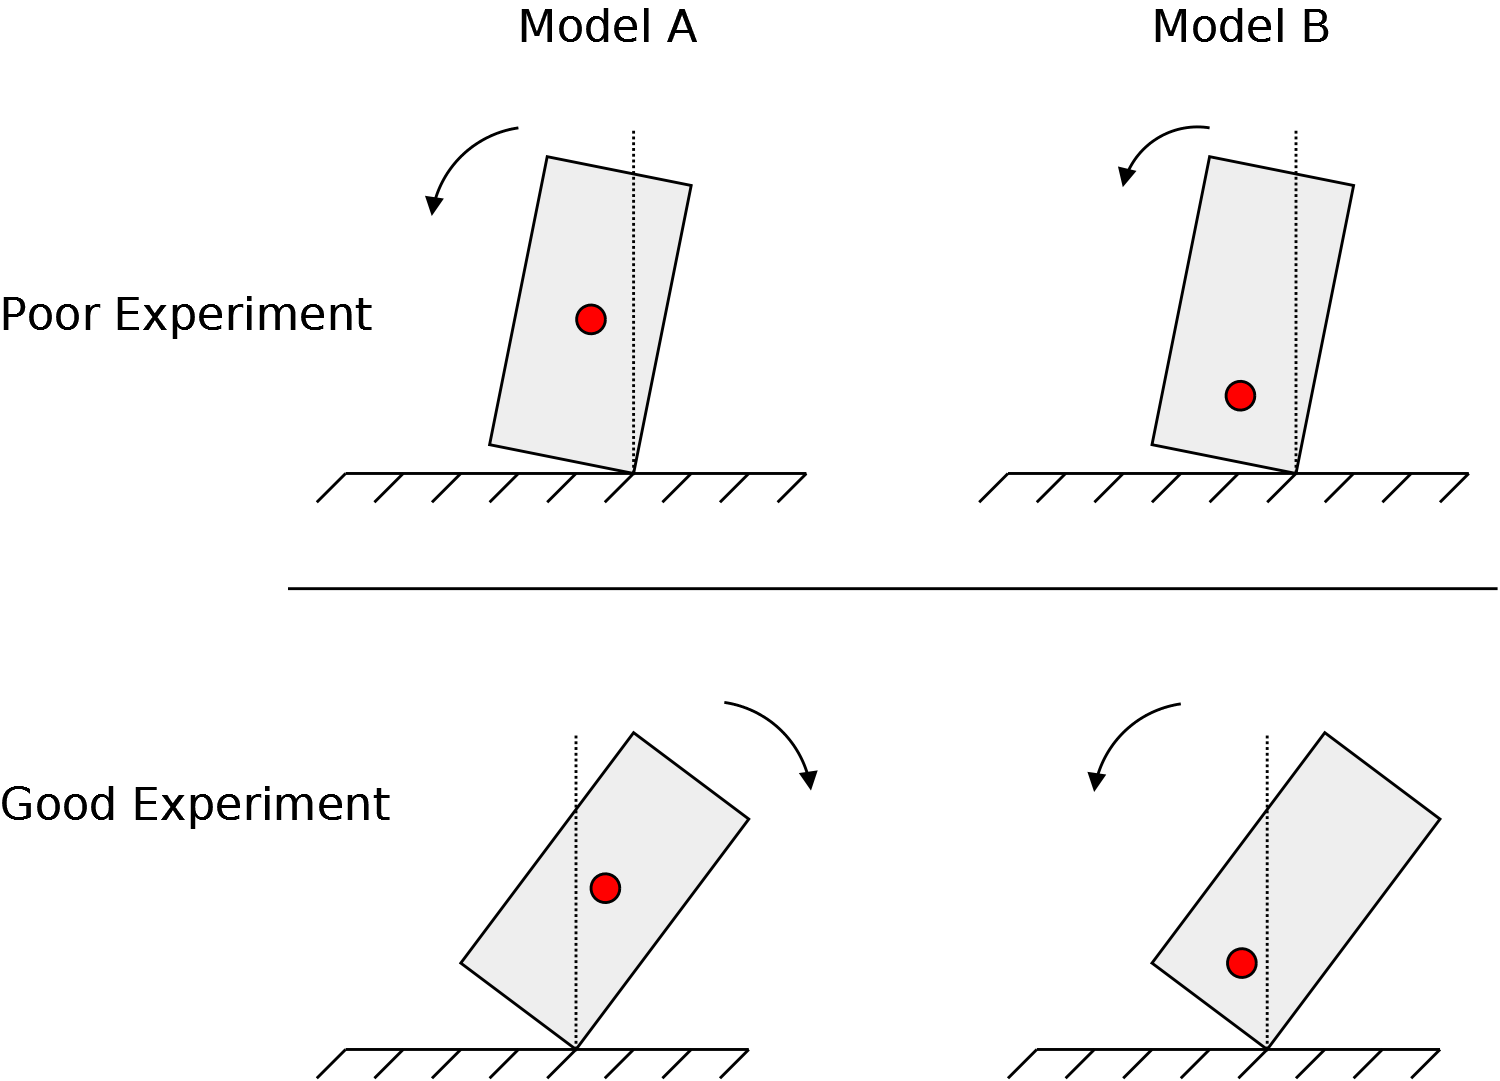
\includegraphics[width=0.7\textwidth]{images/goodvspoor}
\par\end{centering}

\caption{Not all actions that a robot can perform to determine the physical
model of a given object are equally informative. In the above example,
if the robot needs to determine whether the centre of mass of a box
(indicated by the red circles) is located in the middle or at one
of the ends, dropping the box in the top orientation will not provide
much information as the outcome will be the same in both instances
(in both cases the centre of mass is on the same side of the vertical
line drawn from the pivot point). The bottom action is more informative
as the outcome will depend on the centre of mass of the box.\label{fig:Good-and-bad}}
\end{figure}


To determine the information gain of an action we calculate its expected
Kullback-Leibler divergence (KL divergence). KL divergence is a distance
measure between two probability distributions $P$ and $Q$, denoted
as $D_{KL}\left(P,Q\right)$. For discrete probability distributions
P and Q the KL divergence is defined as:

\begin{center}
${\displaystyle D_{KL}\left(P,Q\right)=\underset{i}{\sum}P\left(i\right)\ln\dfrac{P\left(i\right)}{Q\left(i\right)}}$
\par\end{center}

It is formally a measure of the expected number of bits that are needed
to encode samples from one distribution when using a code based on
the other. In Bayesian statistics the KL divergence between two distributions
can be used as measure of the information gained moving from one to
the other. Furthermore, in the domain of Bayesian optimal experimental
design a common aim is to maximise the KL divergence between the
prior and posterior. Such experiments are Bayes d-optimal. In our
system, the robot chooses to perform the experiment with the highest
expected KL divergence from the current confidence distribution, thus
maximising the expected information gain.

\begin{figure}
\begin{centering}
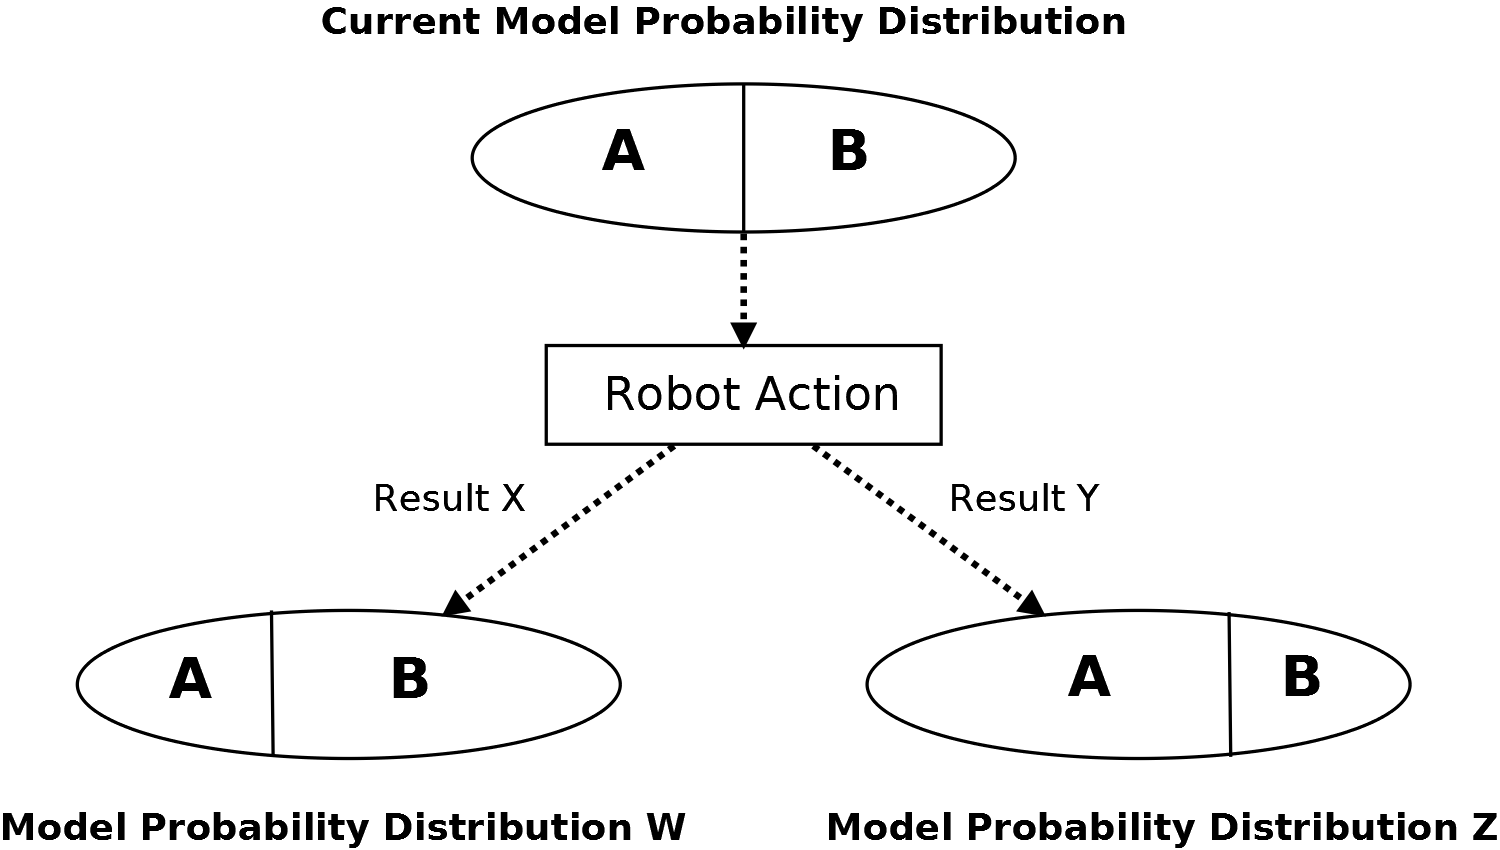
\includegraphics[width=0.7\textwidth]{images/experiment}
\par\end{centering}

\caption{To determine the usefullness of a given action, we find the expected
KL-divergence between the prior probability distribution (Current
Probability Distribution) and the resulting posterior probability
distribution after the action is performed and result known. In the
simple example above (with two possible outcomes $X$ and $Y$, and
two hypothesis models $A$ and $B$) this is equal to $P\left(ResultX\right)D_{KL}\left(CPD,PDW\right)+P\left(ResultY\right)D_{KL}\left(CPD,PDZ\right)$,
where $CPD$ is the current probability distribution, $PDW$ is the
resulting distribution if the outcome is \emph{$X$}, and $PDZ$ is
the resulting distribution if the outcome is $Y$.\label{fig:Expected-KLD}}
\end{figure}


In order to calculate the expected KL divergence of a given action
we use its probability model (presented in Subsection \ref{sub:Experiment-Model})
and the current confidence distribution over object models. The outcome
of an action is some $r\in R$, and for every possible outcome there
is a corresponding new confidence distribution (computed using equation
X in Section Y). To calculate the expected KL divergence, we take
the weighted sum of the KL divergences between the current confidence
distribution and every possible resulting distribution, weighted by
the probability of the corresponding result. Figure \ref{fig:Expected-KLD}
illustrates this concept for a simple example with only two possible
outcomes for some action. Algorithm \ref{alg:Calculating-the-expected}
provides a step by step description of calculating the expected information
gain. 

\begin{algorithm}
\textbf{input:} action $\rightarrow a$

\textbf{input:} set of possible models $\rightarrow H$

\textbf{input:} set of possible results $\rightarrow R$

\textbf{input:} current confidence distribution $\rightarrow C_{current}$

\medskip{}


$expected\_information\leftarrow0$

\textbf{forall} $r$ \textbf{in} $R$

~~~~$weight\leftarrow0$

~~~~$C_{new}=\left\{ c_{1}^{new},c_{2}^{new},\ldots,c_{n}^{new}\right\} $

\textbf{~~~~forall} $h_{i}$ \textbf{in} $H$

~~~~~~~~$weight\leftarrow weight+c_{i}P\left(r|M=h_{i},a\right)$

~~~~~~~~$c_{i}^{new}\leftarrow\dfrac{P\left(r|M=h_{i},a\right)c_{i}^{current}}{P\left(r|a\right)}$

\textbf{~~~~endfor}

\textbf{~~~~}$expected\_information\leftarrow expected\_information+weight\cdot D_{KL}(C_{current},C_{new})$

\textbf{endfor}

\medskip{}


\textbf{output:} expected KL divergence of the action $\leftarrow expected\_information$

\caption{Calculating the expected KL divergence of a given action.\label{alg:Calculating-the-expected}}
\end{algorithm}



\subsection{Relation to Active Machine Learning}

Our system can be viewed as a transformation of a well known active
machine learning approach. Active learning is a form of supervised
machine learning where the algorithm actively queries the supervisor
for labels of specific data points, in order to reduce the training
time and improve accuracy. It is motivated by problems where unlabeled
data is abundant, but labeling each training instance is expensive
and/or time consuming. With active learning the algorithm queries
the supervisor to label the training instances which are most informative.

While there are various query strategy frameworks, in our case the
most relevant is \emph{query-by-committee} (QBC)\cite{6_seung_querybycommittee}.
The QBC framework features a committee of competing classifiers, a
labeled set of training data points on which they are trained, and
an unlabeled set of data points. The aim is to determine the most
accurate classifier. The competing classifiers are used to generate
hypothetical labels for the unlabeled data points. The data point
on which they disagree is considered to be the most informative and
is then queried to be labeled by the supervisor. The outcome of this
query is used to update the accuracy of each classifier. Kullback-Leibler
divergence is one particular method used as a measure of disagreement
between classifier models, for example used for active learning of
document class classification.

Our system can be viewed as a transformed QBC active learning task
if we consider each of the simulated object physics models as a classifier,
each of the actions that can be performed as an unlabeled training
data point, and the robot carrying out a particular action on the
actual object as the supervisor. First we generate hypothetical labels
for each of the actions (unlabeled training data points) by performing
them in simulation with each of the different models (competing classifiers).
The result of each is a probability distribution over result labels.
We use the KL divergence measure to choose the action which produces
the most disagreement. We then query the supervisor to obtain a label,
which in our case is the robot carrying out the chosen action on the
actual object. This label is then used to update the model likelyhood
distribution, indicating the most accurate object model.


\section{Experimental Results\label{sec:Learning-System-Implementations}}

In order to test the effectiveness of the general framework described
in this chapter, we perform three experiments. In the first experiment
(Subsection \ref{sub:Centre-of-Mass}) we show that the mothod can
be used to learn the centre of mass of an object by dropping it from
particular orientations onto a flat surface and observing the results.
The second experiment (Subsection \ref{sub:Wheels-Experiment}) investigates
the application of the framework to the task of learning the wheel
configuration of a box-cart object. This is done by releasing the
box-cart on a sloped ramp in a particular orientation and observing
the trajectory of the cart. The third experiment (Subsection \ref{sub:Stimulus-Response-Behaviour})
demonstrates the general applicability of the learning method by showing
that it can be used to learn object properties not limited to physical
attributes. In this case, the object is a Lego Mindstorms robot programmed
to perform a particular movement behaviour in response to some stimulation.
The stimulation is in the form of activating a light sensor of the
Lego robot. The goal of the main robot is to determine the particular
behaviour model by using a flashlight to illuminate the light sensors
and observing the resulting movement of the Lego robot.

Following the three robot learning experiments, we demonstrate the
benefits of learning a predictive model of an object. This is done
by having the robot plan and perform a tool use task using an object
and a learned physics engine model of that object. This learned model
is used to plan an appropriate action in simulation and then carry
it out to accomplish a goal.


\subsection{Centre of Mass Experiment\label{sub:Centre-of-Mass}}


\subsubsection{Overview}

In this experiment we apply the proposed active robot learning framework
to the task of finding the centre of mass of an object. The robot
is presented with two different objects: a box and a cylinder, and
must determine the centre of mass of each by dropping them onto a
flat surface. The dimensions of the box object are \emph{$5.5cm\times8.4cm\times11.9cm$.}
The cylinder object is \emph{$14cm$} in height (along the z-axis)
and \emph{$5cm$} in diametre (see Figure \ref{fig:Box-and-Can.}).
Both the cylinder and the box may have weights added internally in
order to change the location of their centre-of-mass. The drop orientations
and heights are chosen to have the highest expected information gain
using the previously described method to find the most informative
action from a set of available actions. A physics engine simulator
is used in order to simulate the various possible object models and
actions. 

\begin{figure}
\begin{centering}
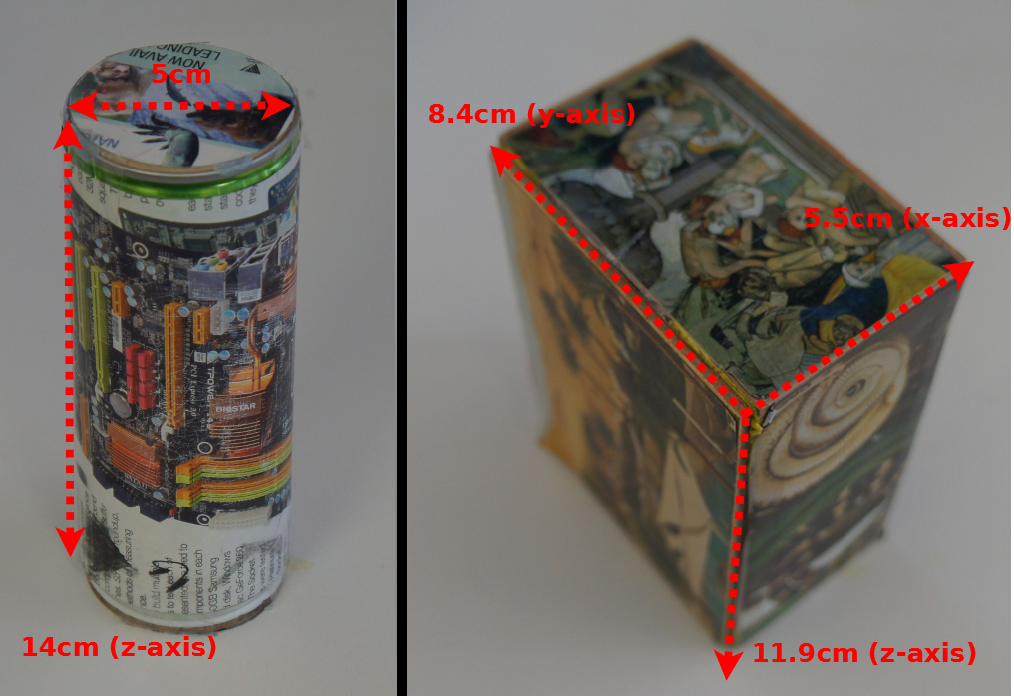
\includegraphics[width=0.6\textwidth]{images/canbox}
\par\end{centering}

\caption{The cylinder (left) and box (right) objects used in the \emph{Centre
of Mass Experiment}. Each can be unweighted, in which case it has
a centre of mass in the centre, or can have weights added internally
to offset the centre of mass.\label{fig:Box-and-Can.}}


\end{figure}


In order to find the centre of mass of the box and cylinder objects,
the robot repeats the following steps:
\begin{enumerate}
\item Localise the target object in the scene;
\item Pick up the object with the robot gripper;
\item Calculate the information gain of each action given the current model
likelyhood distribution;
\item Carry out the most informative action possible by dropping the object
from the appropriate height and orientation;
\item Determine the resulting pose of the object;
\item Classify the resulting pose by matching it to a result label;
\item Update the model likelyhood distribution using the outcome probabilities
of the performed action and the result label.
\end{enumerate}
The object is localised in a scene using the method described in previous
chapter, using a complete aspect graph of SIFT features and a depth
camera. In the case of a box and cylinder objects, grasping is performed
along the longest axis of each object with the vector between the
two gripper pads parallel to the ground plane. Figure \ref{fig:before-after-drop}
shows a before and after image of the robot performing a drop experiment
on the box object.

\begin{figure}
\begin{centering}
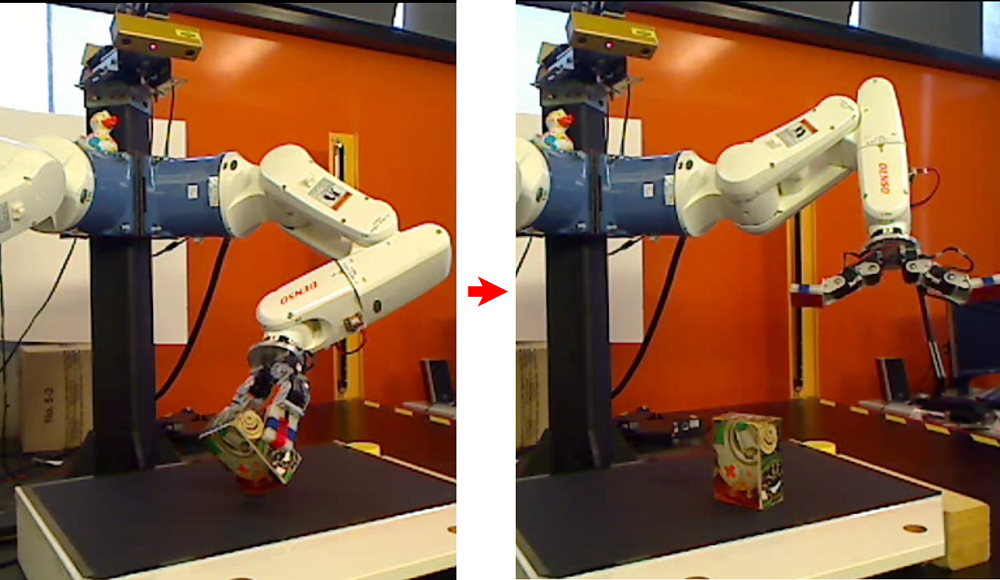
\includegraphics[width=0.8\textwidth]{images/drop_before_after}
\par\end{centering}

\caption{The before (left) and after (right) state of a single iteration of
the \emph{Centre of Mass Experiment}. The robot positions the box
and cylinder objects in an appropriate orientation and height above
the flat table-top, and then releases it. The resulting orientation
of the object provides information on the location of its centre of
mass. \label{fig:before-after-drop}}
\end{figure}


In the remainder of this section we present the following: the possible
models that can describe the objects and the actions that the robot
can perform (Section \ref{sub:Object-Models-and}), the simulation
method used to determine the action probability models (Section \ref{sub:Simulation-Method}),
the method of labeling the result of each drop action with a discrete
label (Section \ref{sub:Result-Classification}), and the performance
results of applying the object model learning method to determining
the centre of mass of a box and cylinder object (Section \ref{sub:Performance-Results2}).


\subsubsection{Possible Object Models and Actions\label{sub:Object-Models-and}}

The goal for the robot is to determine which of the models, from a
pre-defined set of possible models, best fits the object in question.
This is done by performing actions from a pre-defined pool. For this
experiment we define three possible centre-of-mass models for both
the box and cylinder objects (shown in Figure \ref{fig:drop_models}).
In the case of the box object, the possible models have their centre-of-mass
either in the middle of the box or offset half-way along the main
axis. The coordinates (in centimetres) of the centre-of-mass of the
three possible box models are: $(0,0,0)$, $(0,0,3)$, and $(0,0,-3)$.
The coordinate $(0,0,0)$ corresponds to the centre of the box. In
the case of the cylinder object, the possible models also have their
centre-of-mass either in the middle or offset half-way along the main
axis. The coordinates (in centimetres) of the centre-of-mass of the
three possible cylinder models are: $(0,0,0)$, $(0,0,3.5)$, and
$(0,0,-3.5)$. The coordinate $(0,0,0)$ corresponds to the centre
of the cylinder.

The actions that the robot can perform on the box and cylinder is
dropping each from a specified orientation and height. The drop height
is defined as the distance between the flat tablet-top and the nearest
point on the object's surface. The drop orientation is defined as
the upward facing direction of the object at the time of release,
as dropping an object onto a flat surface has rotational symmetry
around the vertical axis. The pool of available actions is specified
\emph{ad hoc} to consist of $100$ instances, each with a randomly
generated drop height (in the range $0.5cm$ to $2cm$) and drop orientation.
The drop height is generated by choosing a random value in the specified
range $[0.5,2.0]$, the drop orientation is generated by choosing
a random unit vector. 

\begin{figure}
\begin{centering}
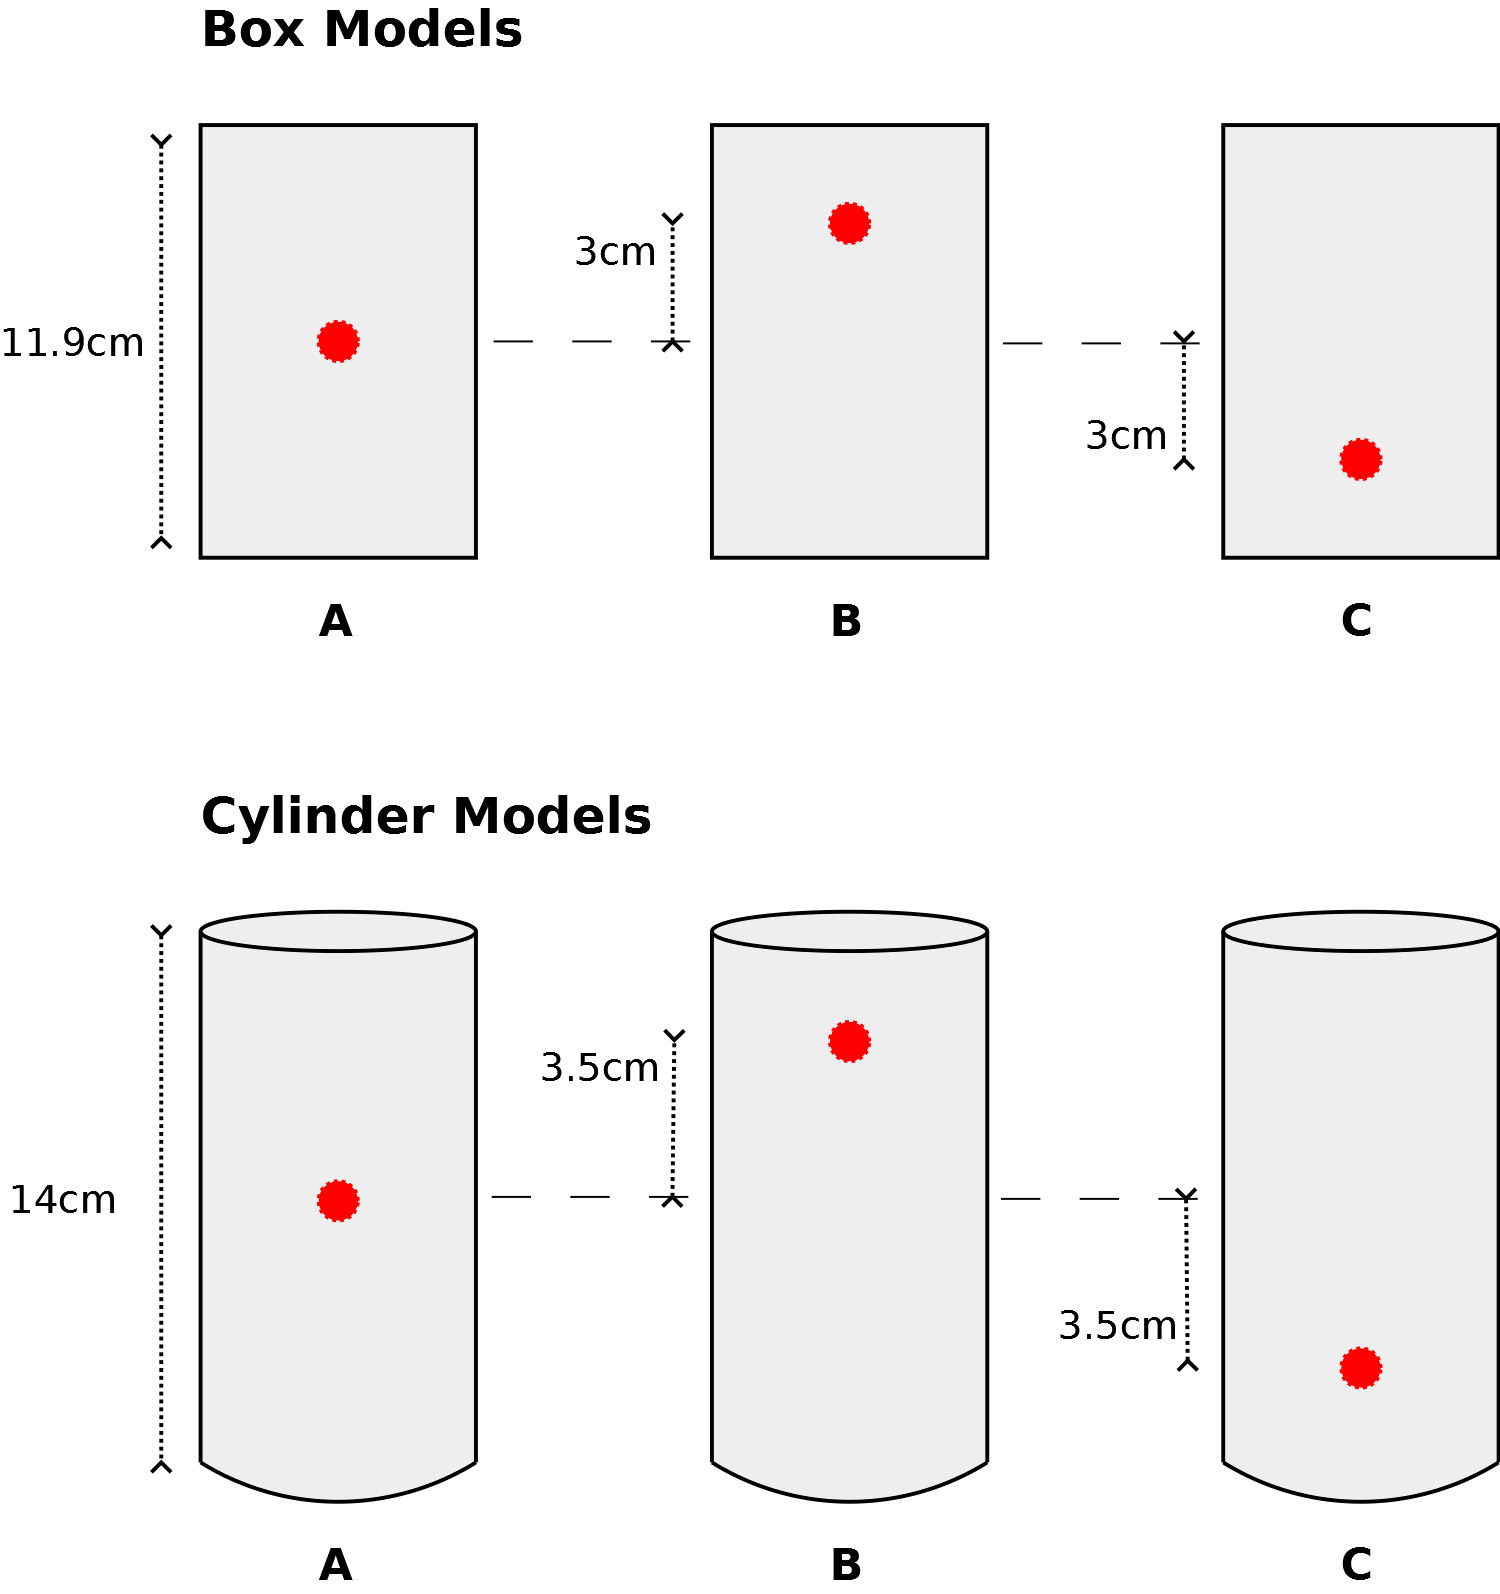
\includegraphics[width=0.7\textwidth]{images/drop_models}
\par\end{centering}

\caption{The potential models for the box and cylinder objects. Each can be
described by one of 3 models, with the centre of mass (denoted by
the red circle) in the middle (model A), or with the centre of mass
offset half way to the end along the longest axis of the object (models
B and C).\label{fig:drop_models}}


\end{figure}



\subsubsection{Simulation Method\label{sub:Simulation-Method}}

Our approach to learning the properties of an object involves simulating
the outcome of various actions performed on the different possible
object models. This is done in order to calculate the action probability
model (ie: the probabilities $P\left(r|h,a\right)$ and $P(r|a)$).
This is then used to update the confidence distribution after an action
is performed and a result observed, as well as to calculate the expected
KL divergence of the different actions in order to perform the most
informative one.

To simulate the actions and find their conditional probability distributions
we use the Bullet Physics Engine%
\footnote{http://www.bulletphysics.com%
} (version 2.76). The Bullet Physics Engine is capable of simulating
the interactions between various bodies. This includes collision detection
between bodies, soft-body and rigid-body dynamics, as well as being
able to simulate various types of joints, hinges, and axles. 

The flat workspace surface is simulated by an infinite plane with
friction set to $1.0$, and the gravity vector set to $(0,0,-9.8)$
$m/s^{2}$. The box and cylinder are simulated by a \emph{ConvexHull
}rigid body, with friction set to $1.0$, restitution parameter set
to $0.01$, linear damping parameter set to $0.05$, and angular damping
set to $0.5$. These parameters were chosen \emph{ad hoc} and result
in realistic looking simulations. The mass of the simulated objects
does not affect the outcome of a simulated actions and is set to $1.0$.

During simulation we simplify the action significantly. We do not
simulate the robot arm grasping the object, moving it into position,
and releasing the object. Instead, the simulated object is set to
the appropriate orientation and height above the ground plane (as
specified by the action parameters) and released. In order to model
the noise and errors resulting from the robot manipulating an object
in the real world, the simulated object's position and orientation
are perturbed from the values specified by the simulated action. Gaussian
noise is added to the drop height with a mean of $0cm$ and standard
deviation of $0.5cm$, while the orientation is rotated around a random
vector by an amount specified by a Gaussian noise variable with mean
$0\textdegree$ and standard deviation of $10\textdegree$. These
values are also chosen \emph{ad hoc} but are generally conservative
in order to over-estimate the errors of the robot manipulation of
the objects.

After settings the simulated object to the appropriate pose, the physics
simulator is run for $300$ frames, each frame corresponding to $\frac{1}{30}$
of a second. Figure \ref{fig:drop-phys-sim} shows a before and after
screenshot of dropping a box object in a physics engine simulation.
At the conclusion of a simulation, the resting pose of the simulated
object then converted to a discrete result label. This is discussed
in the following section.

\begin{figure}
\begin{centering}
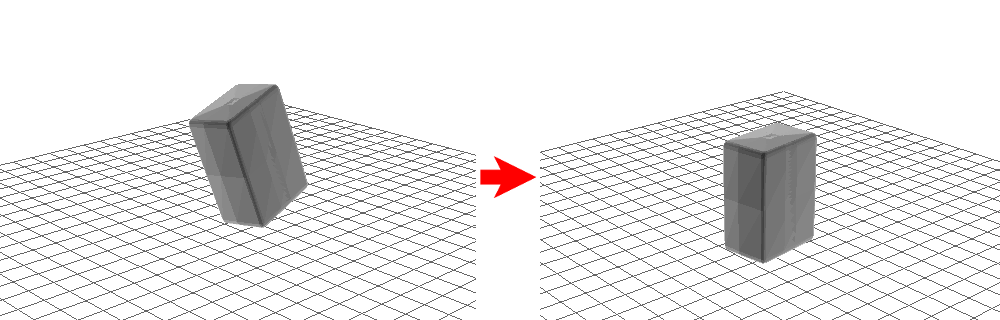
\includegraphics[width=0.8\textwidth]{images/drop0}
\par\end{centering}

\caption{Before (left) and after (right) screenshots of a simulated action,
dropping a box object in a physics engine from a given orientation
and height. The image on the left shows the world state when the box
is released, the right image shows the final pose of the box after
it has come to a stop.\label{fig:drop-phys-sim}}


\end{figure}



\subsubsection{Result Classification\label{sub:Result-Classification}}

Our framework for learning object properties requires that the outcome
of an action is expressed as a discrete result label $r\in R$, where
$R$ is a finite set of all possible result labels (see Section \ref{sub:Result-Labels}).
This is due to the fact that the action model is represented as a
discrete probability distribution over the result labels (see Section
\ref{sub:Experiment-Model}). For a robot action, the outcome is generically
some world state described by a continous variable. By discretising
and extracting the relevant information, this world state can be converted
into a result label.

In the case of dropping an object to find its centre of mass, the
relevant part of the outcome world state is the resting pose of the
object. For effectively classifying the results of a drop, the full
6 degrees of freedom pose of the object is not required. Only the
upward facing direction of the object is needed. The upward direction
vector is calculated using the following formula: 

\begin{center}
$up\_vector=M^{-1}\left(0,0,1\right)^{T}$,
\par\end{center}

where $M$ is the object's world space orientation matrix and $\left(0,0,1\right)^{T}$
is the world ``up'' direction. The next step is to discretise the
outcome up vector of the object in order to form a result label. This
is done by matching the up vector to a predetermined set of result
bins.

There are several ways in which these result bins can be defined.
The most straight forward is to subdivide the unit sphere of up vectors
into uniform sections, with each section corresponding to a result
bin. The outcome result vector would then by matched to the nearest
section. This approach, however, is not optimal for objects such as
a box and cylinder. In the case of a six-sided box, there are only
six possible up vectors that can be the outcome of a drop action (each
corresponding to one of the sides facing upward). Similarly with a
cylinder, only a subset of all up vectors is possible in the outcome.
In this case, the cylinder can have either of its flat ends facing
up, or the rounded side.

In order to generate the appropriate result bins for the \emph{Centre
of Mass Experiment} we take a clustering approach. The reasoning behind
this is to group together up vectors which are logically similar into
the same buckets. This clustering stage is performed at initialisation,
prior to the experiment loop or the building of the action models.
This involves running many simulations of actions on all of the possible
object models, recording the outcome result, and finally clustering
all of the recorded results into bins. This scheme is outlined in
Figure \ref{fig:Result-binning.}. In the case of this experiment,
this is done by taking the outcome up vectors from many simulated
runs, and connecting together vectors which are within $45\textdegree$
of one another. The resulting graph will have multiple connected components,
with each component corresponding to a result bucket. In the case
of the box, there are six connected components, corresponding to the
six sides. In the case of the cylinder, there are three connected
components, two for the flat ends and one for the round side. Each
of these groups of up vectors are stored as a result bucket. In the
remainder of the experiment, when an action is performed (or simulated),
the resulting object up vector is taken and compared against these
result buckets. The result bucket which contains the closest up vector
is taken to be the matching result label $r$.

\begin{figure}
\begin{centering}
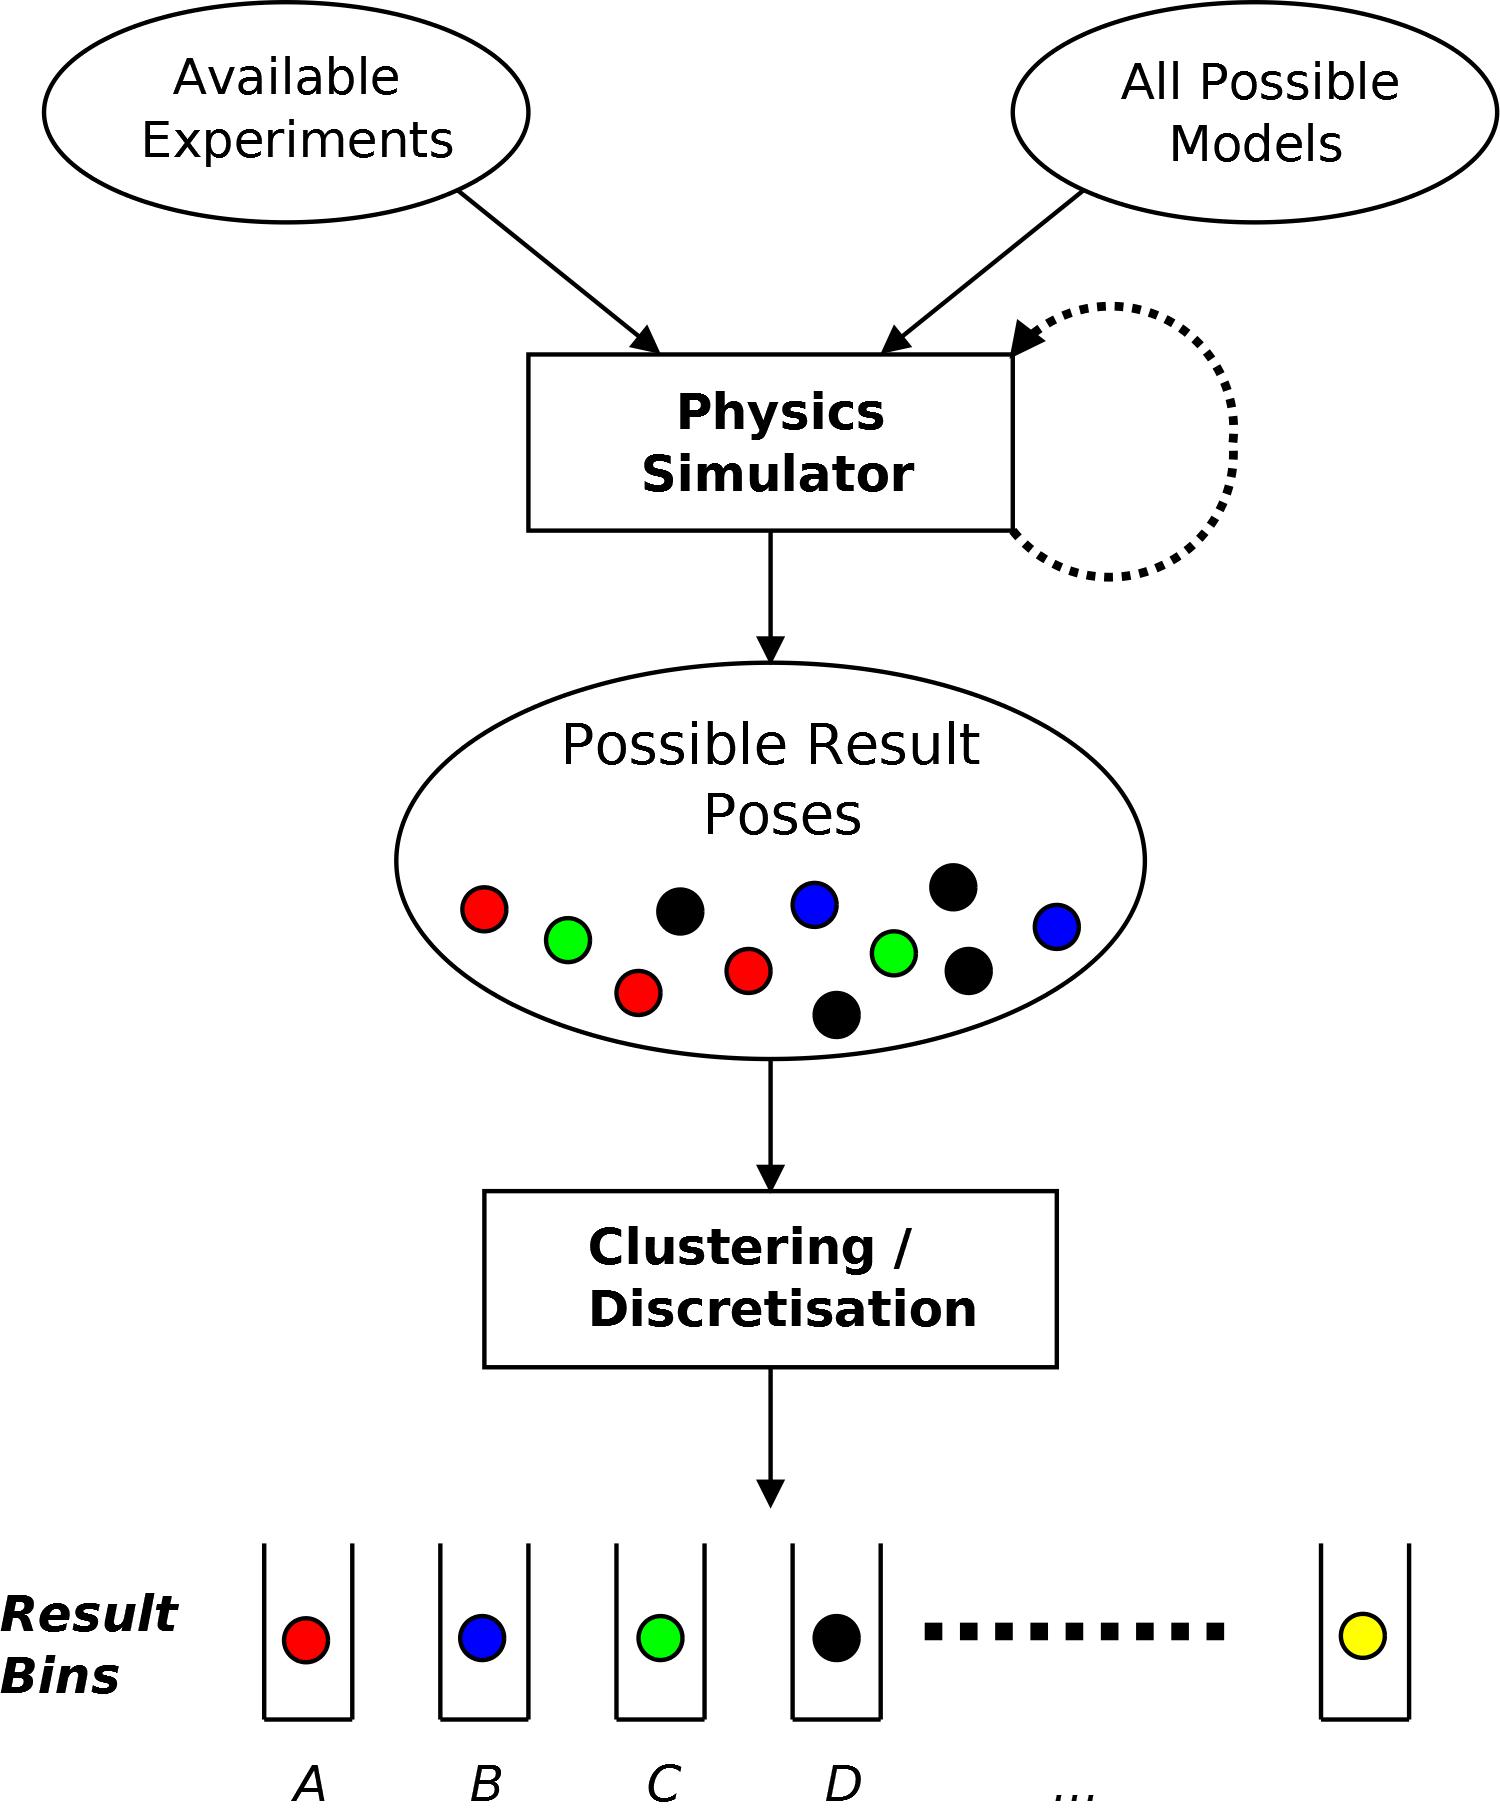
\includegraphics[width=0.6\textwidth]{images/result_bins}
\par\end{centering}

\caption{This diagram outlines how result bins are generated. The available
actions are run multiple times on all of the available object models,
in simulation. The set of output results is then clustered or discretised
to create a smaller set of possible result bins. These are later used
for result labeling. \label{fig:Result-binning.}}
\end{figure}



\subsubsection{Performance Results\label{sub:Performance-Results}}

We test the performance of the learning system by having the robot
carry out multiple runs of learning the object model. In each run
the robot performs a series of actions, updating the confidence distribution
over the possible models using the result of each action. By performing
the most informative action at every stage and using the learned action
models, the robot's confidence distribution should have the matchin
object model's confidence rise to $1.0$ and the remaining models'
confidence fall to $0.0$ as more actions are performed.

The robot performed eight separate trials of determining the object
model of the box. In each trial the robot performed nine drops. This
procedure was done with the box unweighted (centre-of-mass in the
middle), and with the box having weights added internally (centre
of mass offset $-3cm$ from the middle along the z-axis). Figure \ref{fig:Box-drop-experiment}
shows how the robot's model confidence distribution changed during
the nine drops. It can be seen that after even a small number of drops,
the confidence of the object's correct corresponding model rises above
the remaining incorrect models.

\begin{figure}
\begin{centering}
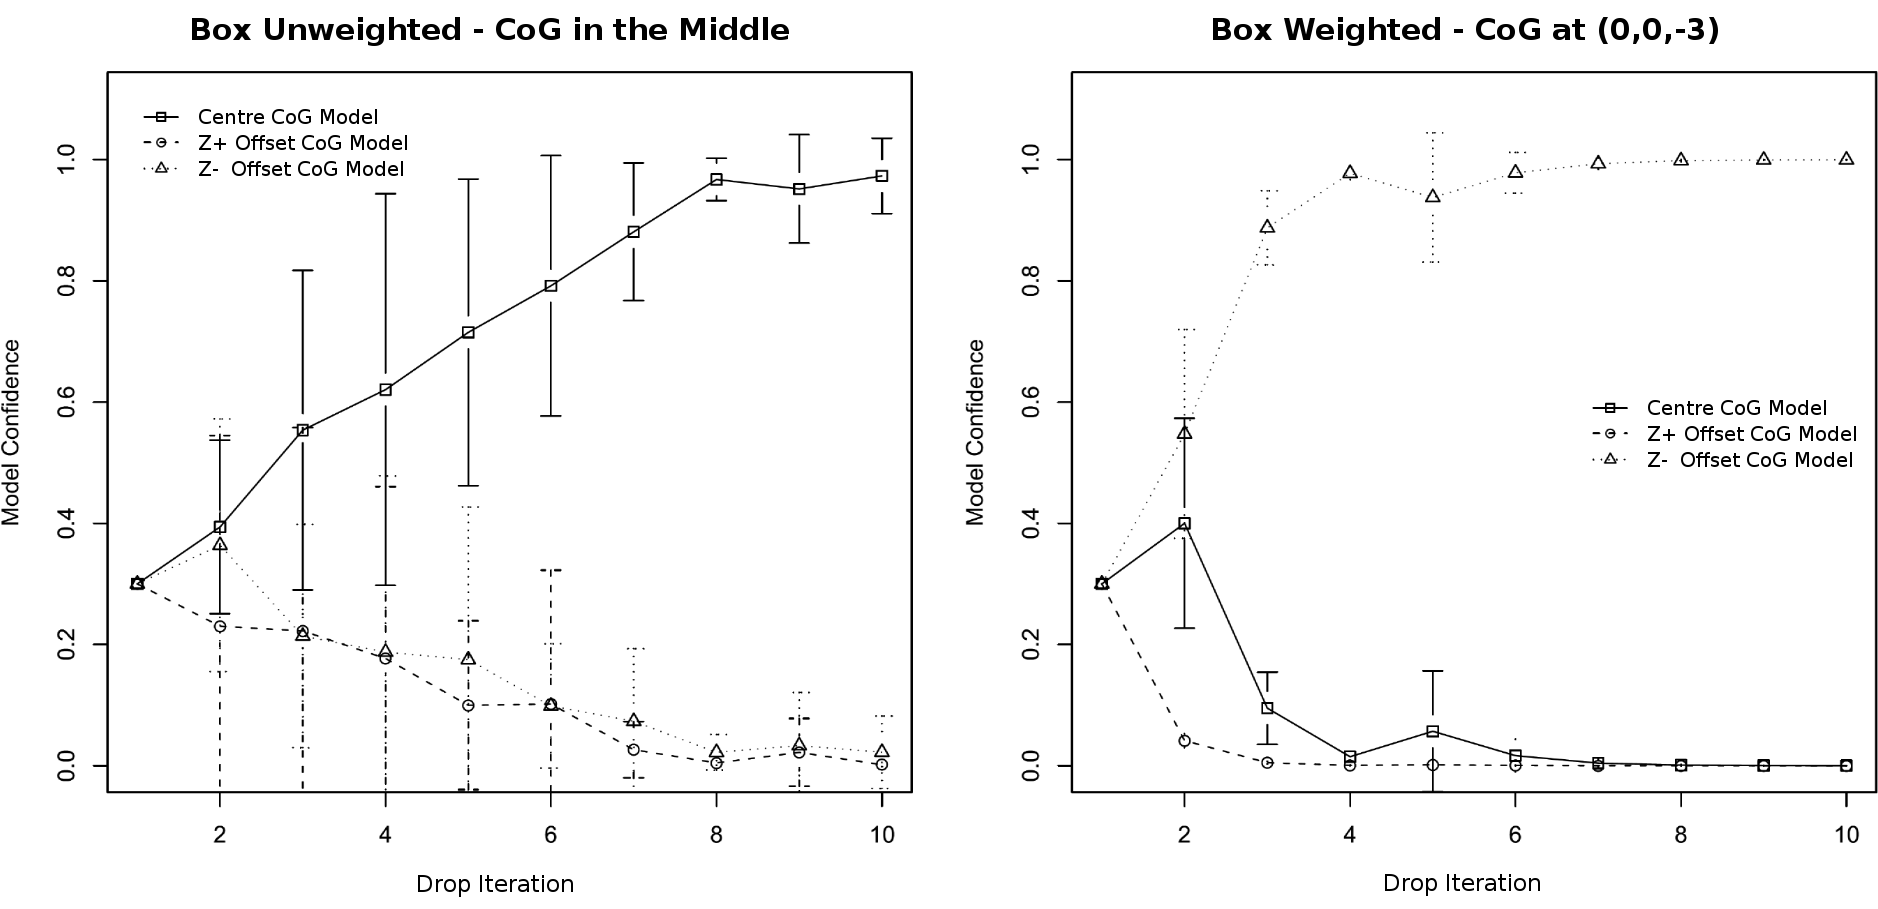
\includegraphics[width=1\textwidth]{images/box}
\par\end{centering}

\caption{The results of the \emph{Centre of Mass Experiment} on the box object,
showing the change in the confidence distribution after a number of
drop iterations. The robot performs multiple drops of the box and
updates its model hypothesis based on the results. The left graph
corresponds to the trials with an unweighted box with the centre of
mass at $(0,0,0)$, with the matching object model indicated as \emph{Central
CoG Model}. The right graph corresponds to the trials with a weighted
box with the centre of mass at $(0,0,3)$, with the matching object
model indicated as \emph{Z+ CoG Model}. The error bars represent the
$95\%$ confidence interval of across 8 independant runs. \label{fig:Box-drop-experiment}}
\end{figure}


With the cylinder object, the robot also performed eight seperate
trials, with each trial consisting of six drops. This is done with
the cylinder unweighted (centre of mass located in the middle), and
with weights added internally (centre of mass offset $-3.5cm$ from
the middle along the z-axis). Figure \ref{fig:Can-drop-experiment.}
shows the change in the confidence distribution over the possible
models during the trials. We can see from the results that the robot
is able to quickly and accurately determine the correct model of the
object by performing the action with the highest information gain.

\begin{figure}
\begin{centering}
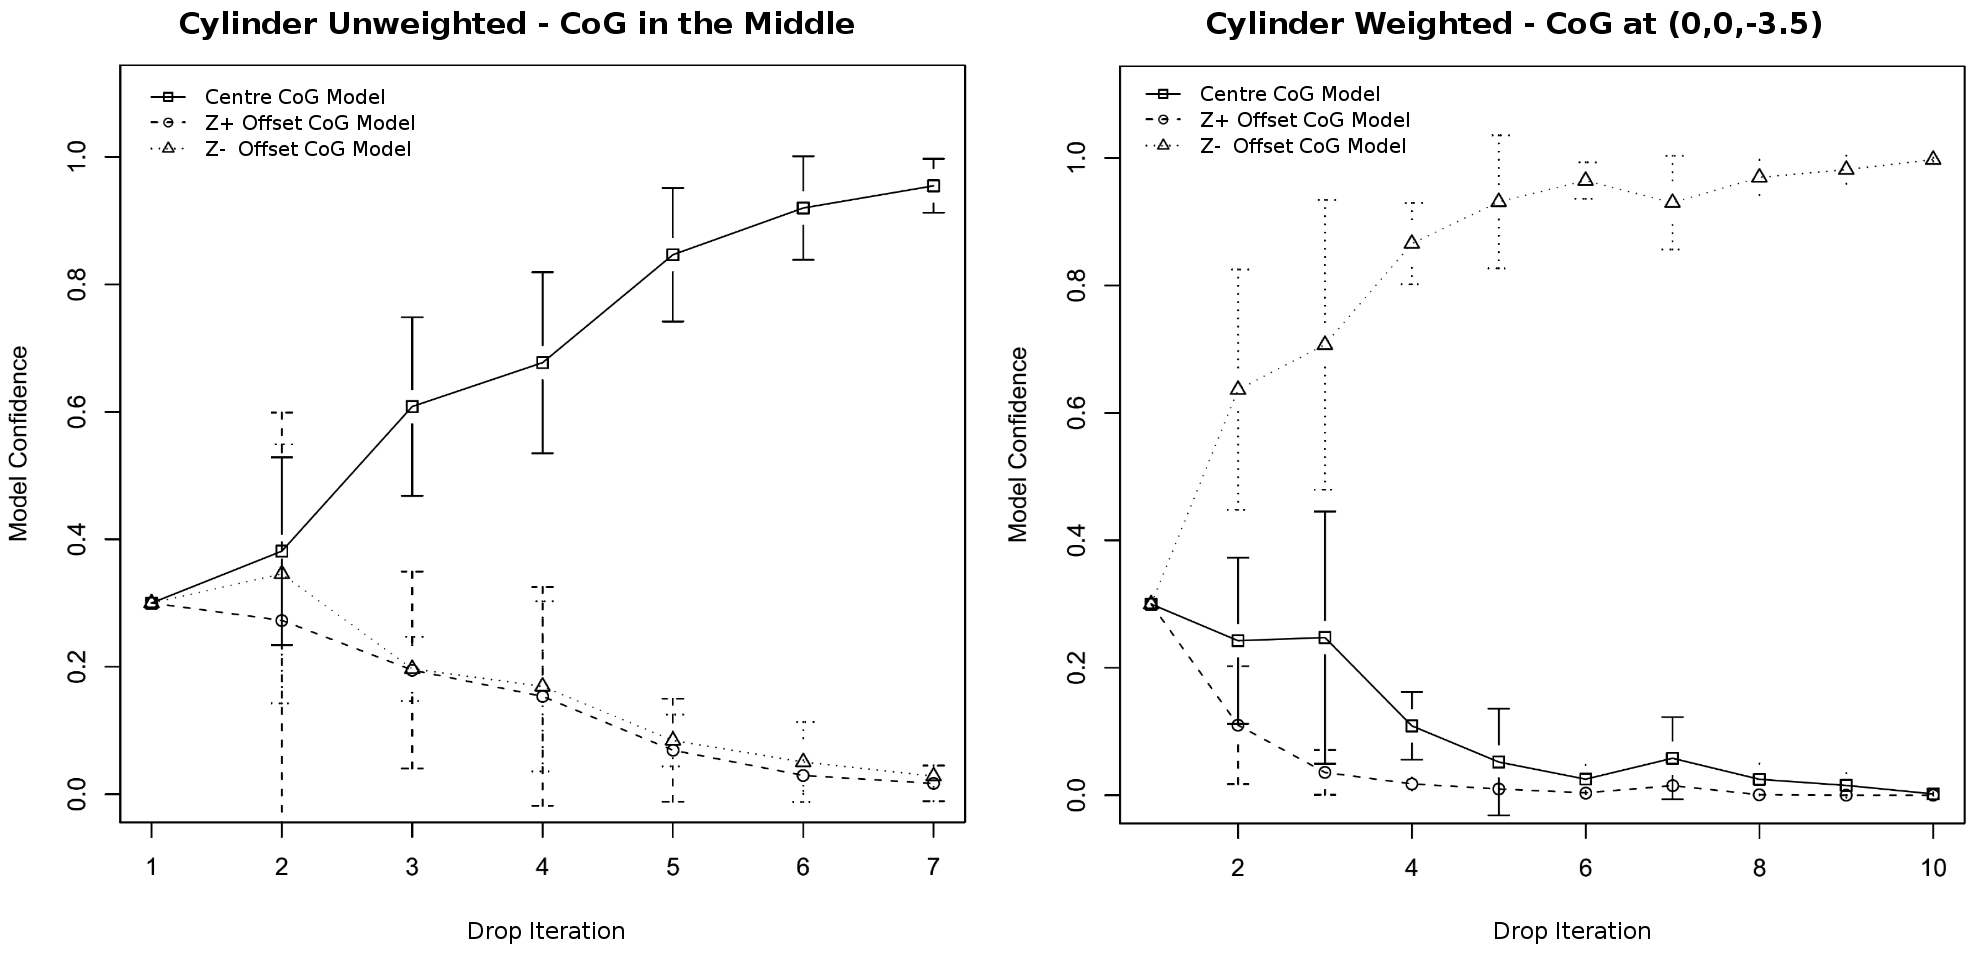
\includegraphics[width=1\textwidth]{images/vcan}
\par\end{centering}

\caption{The results of the \emph{Centre of Mass Experiment} on the cylinder
object, showing the change in the confidence distribution after a
number of drop iterations. The robot performs multiple drops of the
cylinder and updates its model hypothesis based on the results. The
left graph corresponds to an unweighted cylinder with centre of mass
at $(0,0,0)$, the right graph to a weighted cylinder with the centre
of mass offset to $(0,0,-3.5)$ along the main axis. The error bars
represent the standard deviation of the hypothesis across 8 independant
runs.\label{fig:Can-drop-experiment.}}
\end{figure}


In additional to evaluating the performance of the active learning
framework when applied to determining the centre of mass of an object,
we investigated the effect of choosing the action with highest expected
information gain on the learning rate. A key part of the learning
framework is choosing to perform the most informative action, as measure
by the expected KL divergence from the current confidence distribution.
To demonstrate the effect, we compare in simulation a robot learning
the centre of mass of a box and cylinder objects using the most informative
action at every step, and using a random action at every step. It
is important to note that this is carried out purely in simulation,
the actions are simulated in the same manner as when building the
action model. For the best action and random action selection policies,
three simulated runs are performed, each with nine drop actions performed.
The progression of the confidence distribution over the possible object
models is show in Figure \ref{fig:box-action-sim} for the box object,
and in Figure \ref{fig:cylinder-action-sim} for the cylinder object.
It can be seen that by choosing the most informative action leads
to a much faster convergence of the confidence distribution to the
correct object model, whereas choosing a random action leads to much
worse performance.

\begin{figure}
\begin{centering}
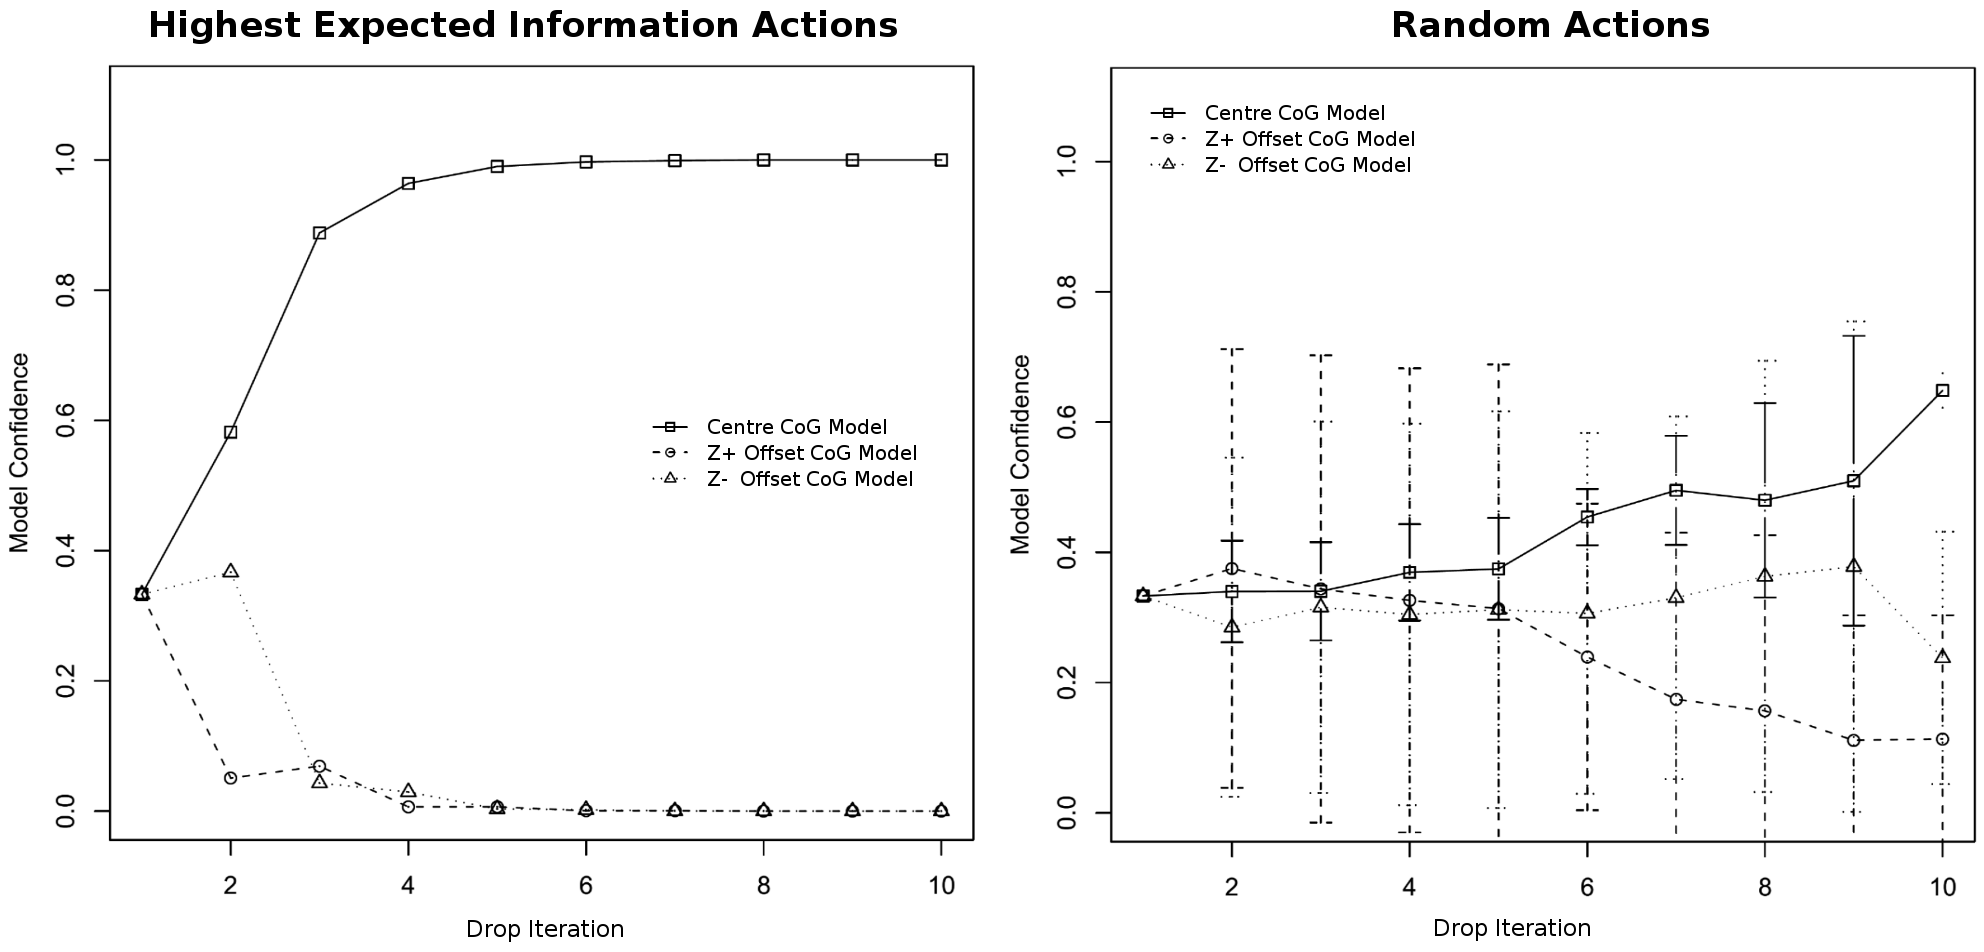
\includegraphics[width=1\textwidth]{images/box_sim}
\par\end{centering}

\caption{Learning the box centre of mass using the action with highest expected
information gain (left), and using a random action (right) at every
iteration. This is performed in simulation, and simulated box has
its centre of mass in the centre (corresponding to the Centre CoG
Model). It can be seen that by performing the most informative action
the confidence distribution quickly converges on the correct object
model. When performing a random action, the confidence distribution
on average does not converge. The error bars indicate the $95\%$
confidence interval.\label{fig:box-action-sim}}


\end{figure}


\begin{figure}
\begin{centering}
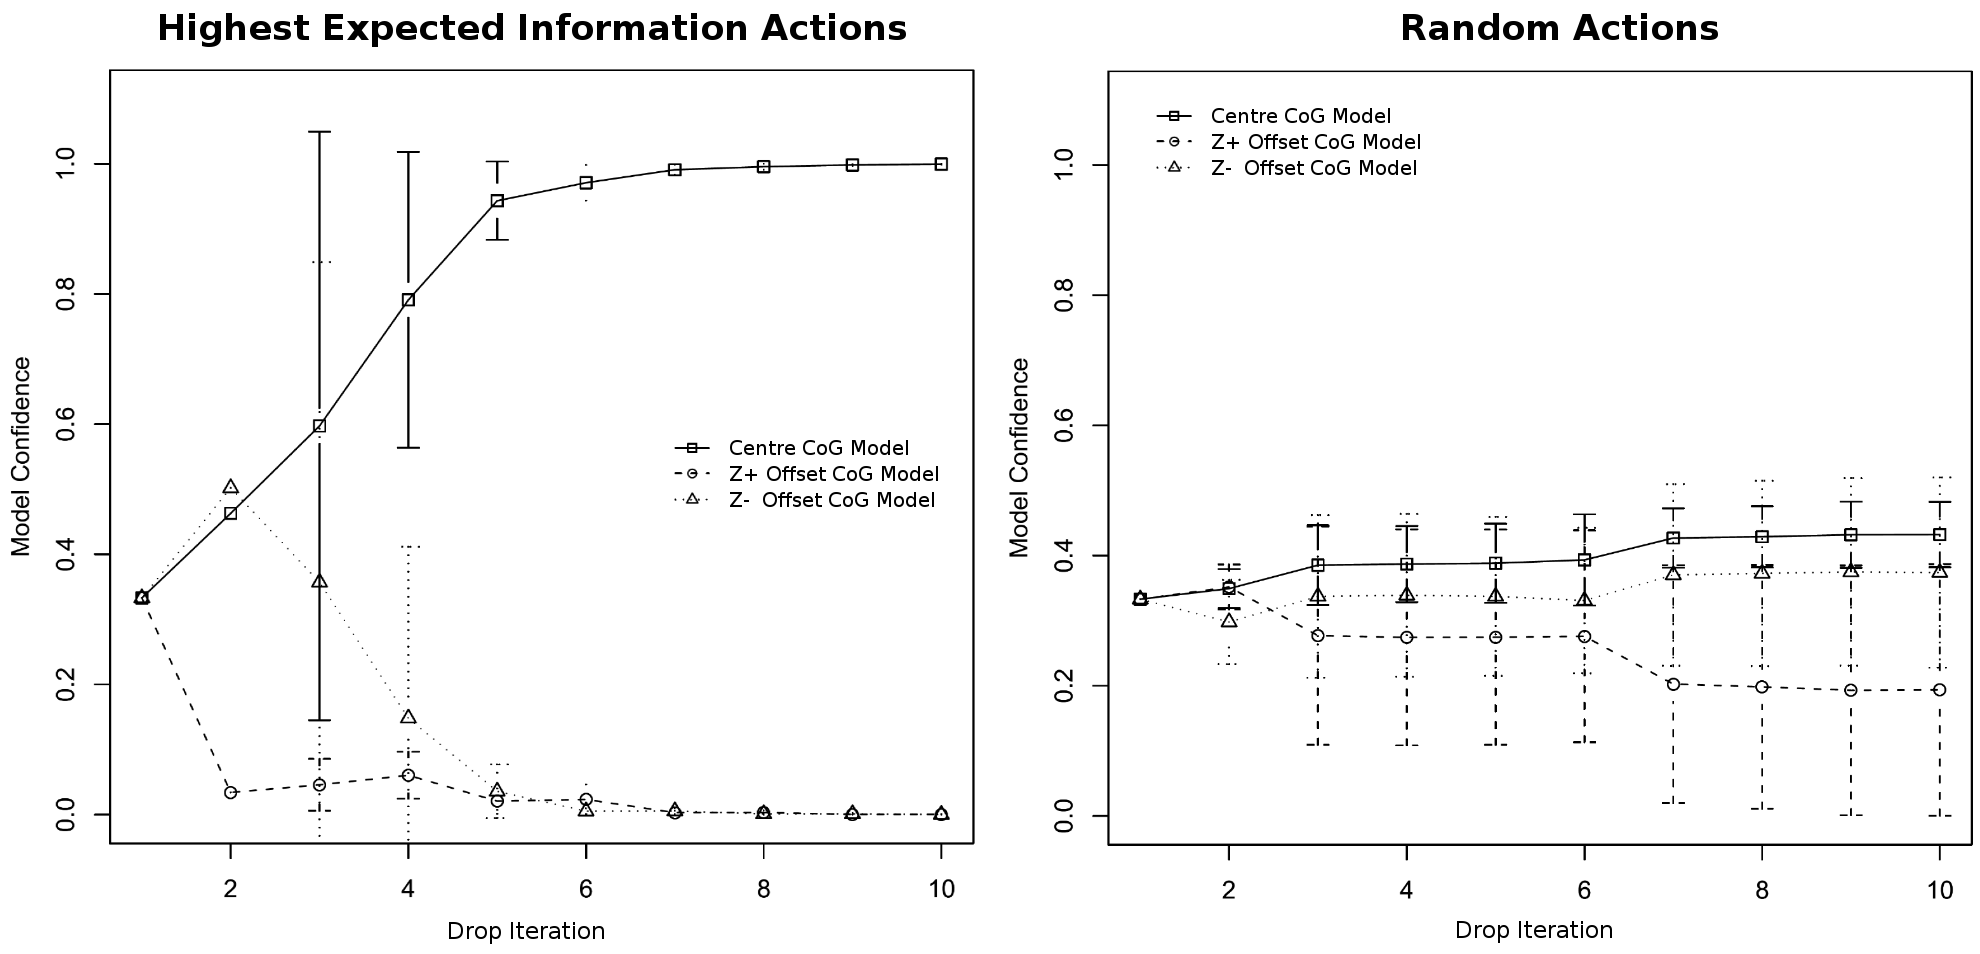
\includegraphics[width=1\textwidth]{images/can_sim}
\par\end{centering}

\caption{Learning the cylinder centre of mass using the action with highest
expected information gain (left), and using a random action (right)
at every iteration. This is performed in simulation, and simulated
cylinder has its centre of mass in the centre (corresponding to the
Centre CoG Model). It can be seen that by performing the most informative
action the confidence distribution quickly converges on the correct
object model. When performing a random action, the confidence distribution
on average does not converge. The error bars indicate the $95\%$
confidence interval.\label{fig:cylinder-action-sim}}


\end{figure}



\subsection{Wheel Configuration Experiment\label{sub:Wheels-Experiment}}


\subsubsection{Overview}

In this experiment we apply the active robot learning framework to
the task of learning the configuration of the wheels on a box-cart
(pictured in Figure \ref{fig:Wheels-object.}). The box-cart consists
of a rectangular prism body, two wheels attached at one end, and a
wooden block at the other. The configuration of the two wheels is
unknown to the robot, specifically how they are oriented and whether
they are able to rotate. For this experiment the workspace consists
of a flat surface and a $25\textdegree$ ramp at one end (see Figure
\ref{fig:Wheels-experiment-layout.}). The robot determines the configuration
of a given box-cart by releasing it on the sloped ramp from various
orientations and observing the resulting resting pose of the object.
By choosing the release pose with the highest expected information
gain, the robot is able to efficiently determine the object model
which matches the box-cart. To choose an optimal action and to update
the model confidence distribution, a physics engine simulator is used
to simulate the outcome of the various actions on the possible object
models.

\begin{figure}
\begin{centering}
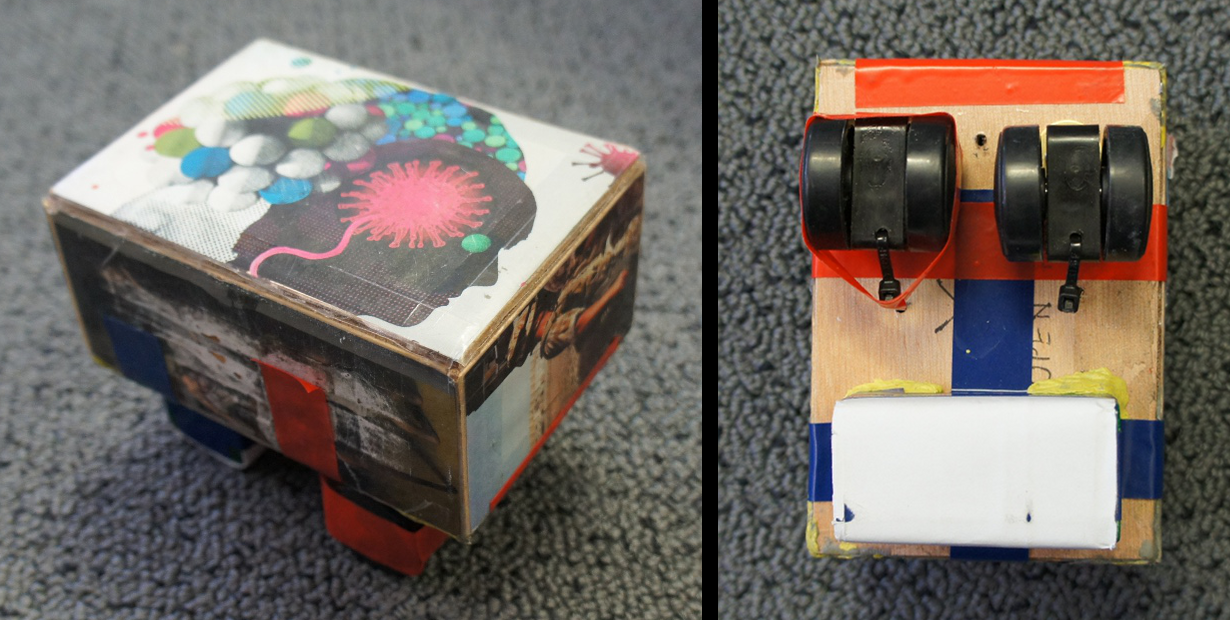
\includegraphics[width=0.7\textwidth]{images/wheels}
\par\end{centering}

\caption{The box cart object used for the \emph{Wheel Configuration Experiment}.
The cart consits of a box, two wheels on one end, and a wooden block
on the opposite end. The wheels can be set to point straight ahead
or $90\textdegree$ to the side. The wheels may also be prevented
from rotating by the application of sticky-tape.\label{fig:Wheels-object.}}
\end{figure}


\begin{figure}
\begin{centering}
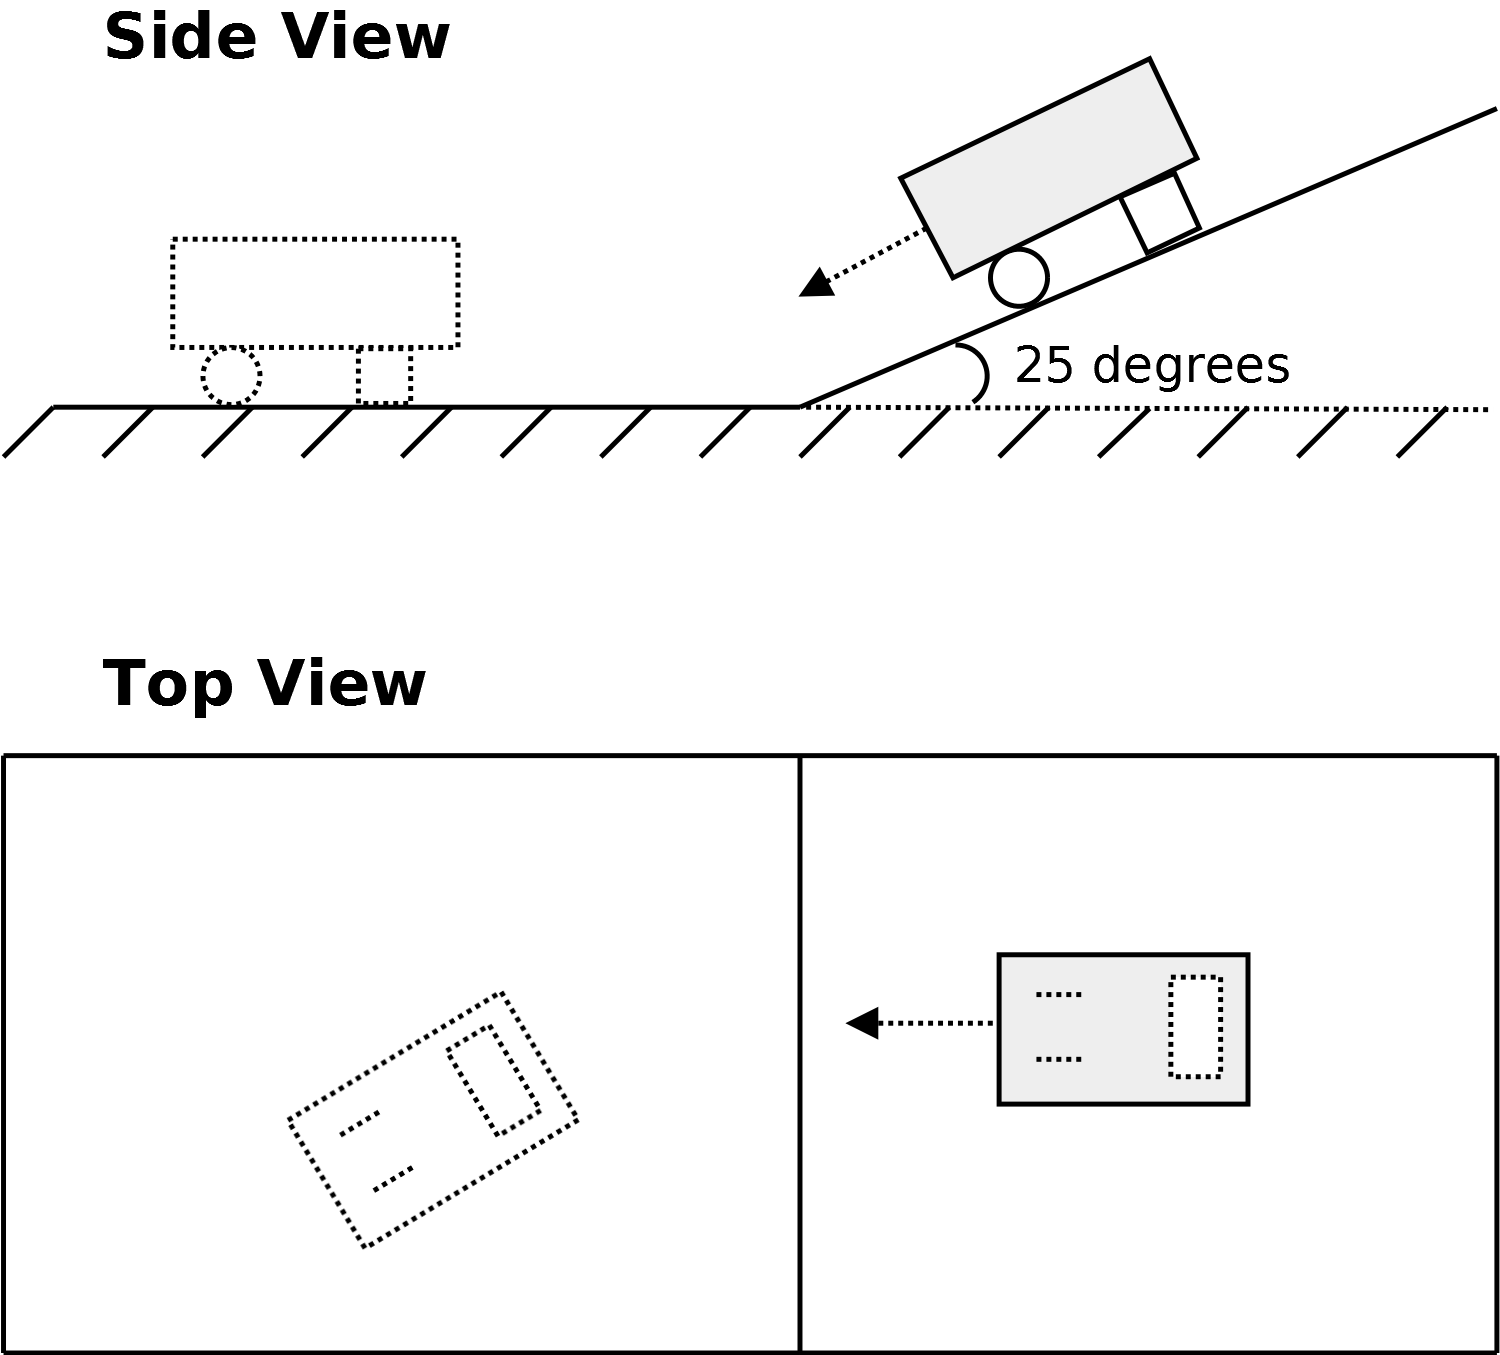
\includegraphics[width=0.6\textwidth]{images/wheels_experiment}
\par\end{centering}

\caption{The workspace layout for the \emph{Wheel Configuration Experiment}.
The robot sets the box-cart down on a $25\textdegree$ ramp and releases
it, allowing it to roll down. The final pose of the cart provides
the robot with information regarding the configuration of the wheels.\label{fig:Wheels-experiment-layout.}}
\end{figure}


The procedure followed by the robot in this experiment is very similar
to that of the \emph{Centre of Mass Experiment}. In order to find
the wheel configuration of the box-cart, the robot repeats the following
steps:
\begin{enumerate}
\item Localise the target box-cart in the scene;
\item Pick up the cart with the robot gripper;
\item Calculate the information gain of each action given the current model
likelyhood distribution;
\item Carry out the most informative action possible by releasing the cart
from the appropriate pose on the ramp;
\item Determine the resulting pose of the cart;
\item Classify the resulting pose by matching it to a result label;
\item Update the model likelyhood distribution using the outcome probabilities
of the performed action and the result label.
\end{enumerate}
The cart is localised in a scene using the method described in previous
chapter, using a complete aspect graph of SIFT features and a depth
camera. Grasping is performed along the longest axis of the top of
the cart, with the vector between the two gripper pads parallel to
the ground plane. Figure \ref{fig:before-after-cart} shows a before
and after image of the robot performing a drop experiment on the box
object.

\begin{figure}
\begin{centering}
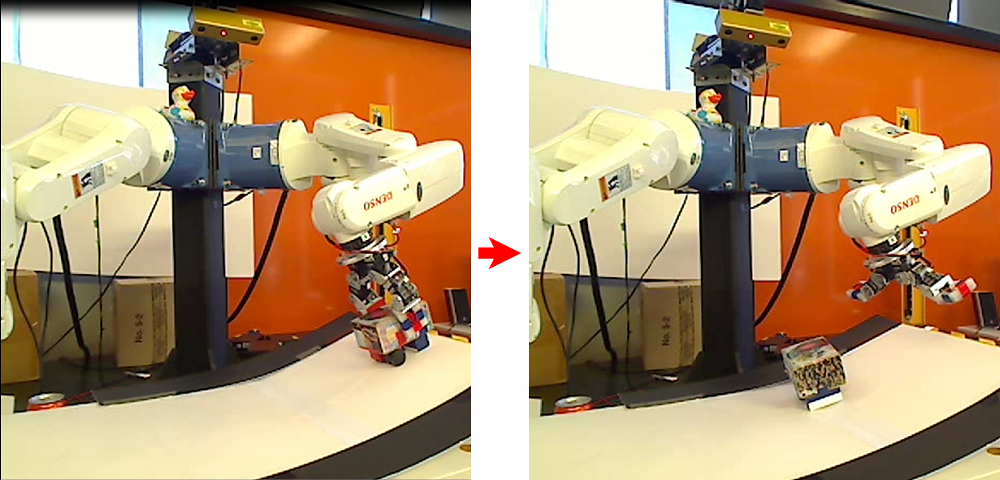
\includegraphics[width=0.8\textwidth]{images/roll_before_after}
\par\end{centering}

\caption{The before (left) and after (right) state of a single iteration of
the \emph{Wheel Configuration Experiment}. The robot positions the
box-cart object in an appropriate orientation and position on the
sloped ramp, and then releases it. The resulting pose of the cart
provides information on the configuration of its wheels.\label{fig:before-after-cart}}
\end{figure}


In the remainder of this section we present the following: the possible
models that can describe the box-cart and the actions that the robot
can perform (Section \ref{sub:Object-Models-and1}), the simulation
method used to determine the action probability models (Section \ref{sub:Simultion-Method1}),
the method of labeling the result of each action with a discrete label
(Section \ref{sub:Result-Classification1}), and the performance results
of applying the object model learning method to determining the wheel
configuration of a cart object (Section \ref{sub:Performance-Results1}).


\subsubsection{Possible Object Models and Actions\label{sub:Object-Models-and1}}

The robot's aim is to determine which model from a predefined set
of models best fits the box-cart. For this experiment we define the
set of possible models to consists of six different wheel configurations
(see Figure \ref{fig:Wheels-experiment-models.}). The two wheels
of the box-cart may both be pointing straight ahead or both $90\textdegree$
to the side, and they may freely rotate or either of the two wheels
may be taped shut (but not both).

\begin{figure}
\begin{centering}
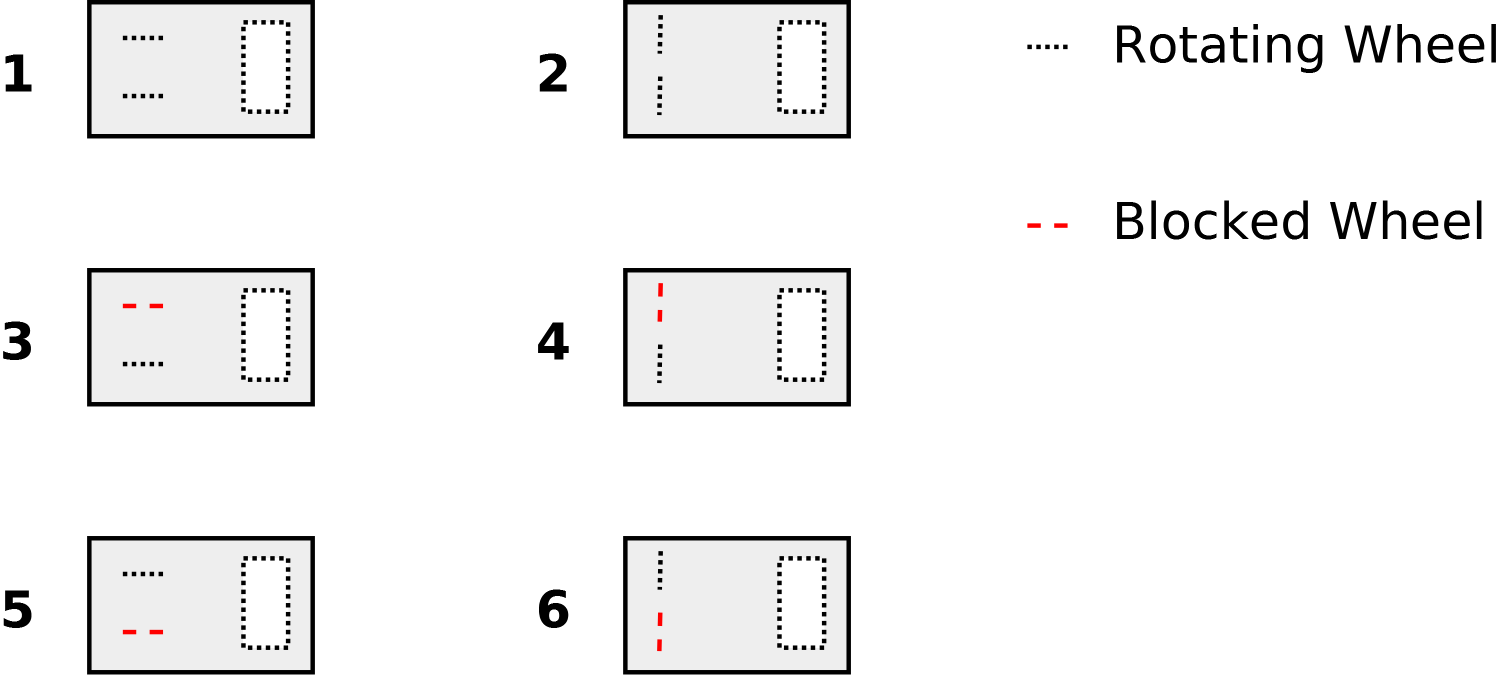
\includegraphics[width=0.8\textwidth]{images/wheels_models}
\par\end{centering}

\caption{The above diagram depicts the 6 different potential models of the
box-cart. Models 1, 3, and 5 have wheels oriented in the direction
of the main axis, models 2, 4, and 6 have wheels oriented at $90\textdegree$
to the main axis. Models 1 and 2 have freely rotating wheels, models
3 and 4 have the right wheel blocked (prevented from rotating), models
5 and 6 have the left wheel blocked.\label{fig:Wheels-experiment-models.}}
\end{figure}


The actions that the robot can perform are in the form of releasing
the cart on the ramp at a predetermined vertical height and orientation.
The cart's wheels and rear block are in contact with the ramp surface
at the time of release. The vertical height of the release is defined
as the vertical distance from the ground plane of the centre of the
cart. The orientation of the cart is defined as the angle it is facing
in the horizontal plane at the time of release. The pool of available
actions is specified \emph{ad hoc} to be $210$ actions. These uniformly
consist of $7$ different release heights between $2cm$ and $8cm$
(in $1cm$ increments), and at each height $30$ possible orientations
in $12\textdegree$ increments.


\subsubsection{Simultion Method\label{sub:Simultion-Method1}}

As with the \emph{Centre of Mass Experiment}, in order to determine
the probability models (ie: the probabilities $P\left(r|h,a\right)$
and $P(r|a)$) for each action, we use the Bullet Physics Engine to
simulate the outcome for each possible action on each possible object
model.

The ramp and flat table surface are simulated with two planes with
friction coefficient set to $0.7$, the gravity vector set to $(0,0,-9.8)$
$m/s^{2}$. The box-cart object is simulated by two box objects for
the main body and rear block, and two cylinder objects for the wheels.
The rear block object is joined to the main box object by a rigid
6 degrees of freedom constraint, forcing them to behave as a single
rigid body. The two cylinders are joined to the box object by hinge
constraints. The direction of the hinge constraint is defined by the
particular model being simulated (whether the wheels of the model
are pointing ahead or to the side). The rear block and wheel friction
coefficient is set to $0.7$. The mass of the main box object is set
to $150$ grams and the mass of each wheel and the rear block is set
to $20$ grams; this matches the measured weight of the real world
box-cart components. The angular damping parameter of each wheel is
set to either $0.15$ or $1.0$, depending on whether the wheel in
the particular model being simulated is free to rotate or not. 

As with the \emph{Centre of Mass}\emph{\noun{ }}\emph{Experiment},
we simplify the action during simulation. Instead of simulating the
robot arm grasping the object and moving it into position, the simulated
object is directly set to the appropriate orientation and position
on the ramp, as specified by the particular action parameters. When
the robot performs an action in the real world, there are multiple
sources of noise and error which affect the outcome. This includes
errors in the positioning of the box-cart on the ramp, slight variations
in the ramp and tabletop surface, variations in the wheel axle's turning
resistance, etc. In order to account for these sources of noise when
performing a simulated action, we perturb the release height and orientation,
as well as perturbing the axle damping parameters for each wheel.
The release height and orientation are perturbed by Gaussian noise
with mean $0$ and standard deviation set to $0.5cm$ and $10\textdegree$
respectively. The wheel damping parameters, wheel friction, and rear
block friction are each perturbed by uniform noise in the range $[-0.1,0.1]$.

After settings the simulated box-cart to the appropriate pose, the
physics simulator is run for $300$ frames, each frame corresponding
to $\frac{1}{30}$ of a second. Figure \ref{fig:cart-phys-sim} shows
a before and after screenshot of a release action carried out in physics
engine simulation. At the conclusion of a simulation, the resting
pose of the simulated object then converted to a discrete result label.
This is discussed in the following section.

\begin{figure}
\begin{centering}
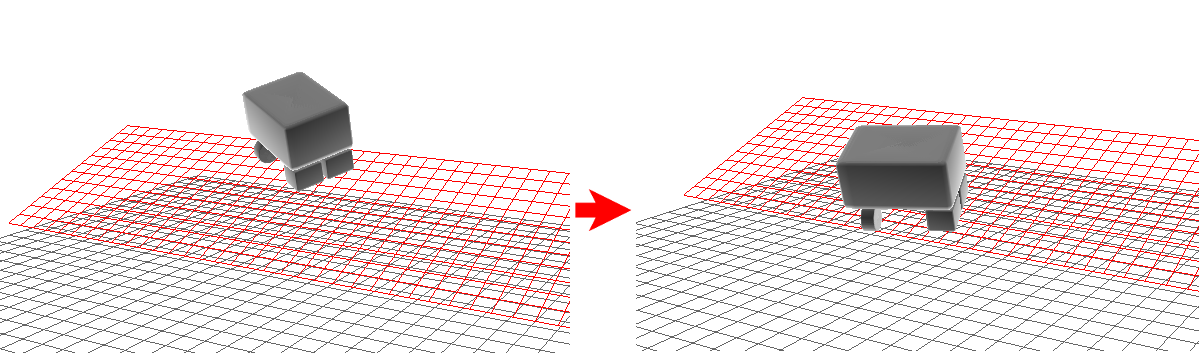
\includegraphics[width=0.8\textwidth]{images/wheels_sim}
\par\end{centering}

\caption{Before (left) and after (right) screenshots of a simulated action,
releasing a box-cart object on a ramp in a the physics engine. The
image on the left shows the world state when the box-cart is released,
the right image shows the final pose of the box-cart after it has
come to a stop.\label{fig:cart-phys-sim}}


\end{figure}



\subsubsection{Result Classification\label{sub:Result-Classification1}}

Our method for learning object properties requires that the outcome
of an action is a discrete result label $r\in R$. This is done by
discretising and extracting the relevant information from the outcome
world state of an action. In the case of this Wheel Configuration
Experiment, the discretisation is performed by matching the resulting
pose of the box-cart after it has rolled down the ramp and come to
rest. The resting pose is constrained to be on the surface of the
flat tabletop or ramp, and we assume the box-cart remains upright.
Therefore we can simplify the full six degrees of freedom cart pose
by expressing the result as the $(x,y)$ position and an angle $\theta$
for the orientation of the cart on the tabletop plane. For labeling
the simplified pose we use a uniform discretisation scheme. The workspace
is divided into cells, $3cm\times3cm$ in size, and orientations are
divided into $10\textdegree$ increments. Each of these cells corresponds
to a single result bin. A given $(x,y,\theta)$ result pose can be
mapped to a result bin by finding the particular cell which contains
the result pose. The matching cell for a given box-cart pose is taken
to be the result label $r$.


\subsubsection{Performance Results\label{sub:Performance-Results1}}

We test the performance of the learning system by having the robot
carry out multiple runs of learning the box-cart model. In each run
the robot performs a series of actions, updating the confidence distribution
over the possible models using the result of each action.

The robot performed six separate trials of determining the object
model of the box. In each trial the robot rolled the cart down the
ramp six times. This was repeated with the box-cart's wheels set to
all six of the possible configurations (see Figure \ref{fig:Wheels-experiment-models.}).
The results of these trials are presented in Figure \ref{fig:Wheels-ramp-experiment.},
showing how the robot's model confidence distribution changed during
the course of the trials. Each of the separate graphs correlates to
a different configuration of the box-cart object. It can be seen that
very quickly the confidence of the object's correct corresponding
model rises above the remaining incorrect models. 

\begin{figure}
\begin{centering}
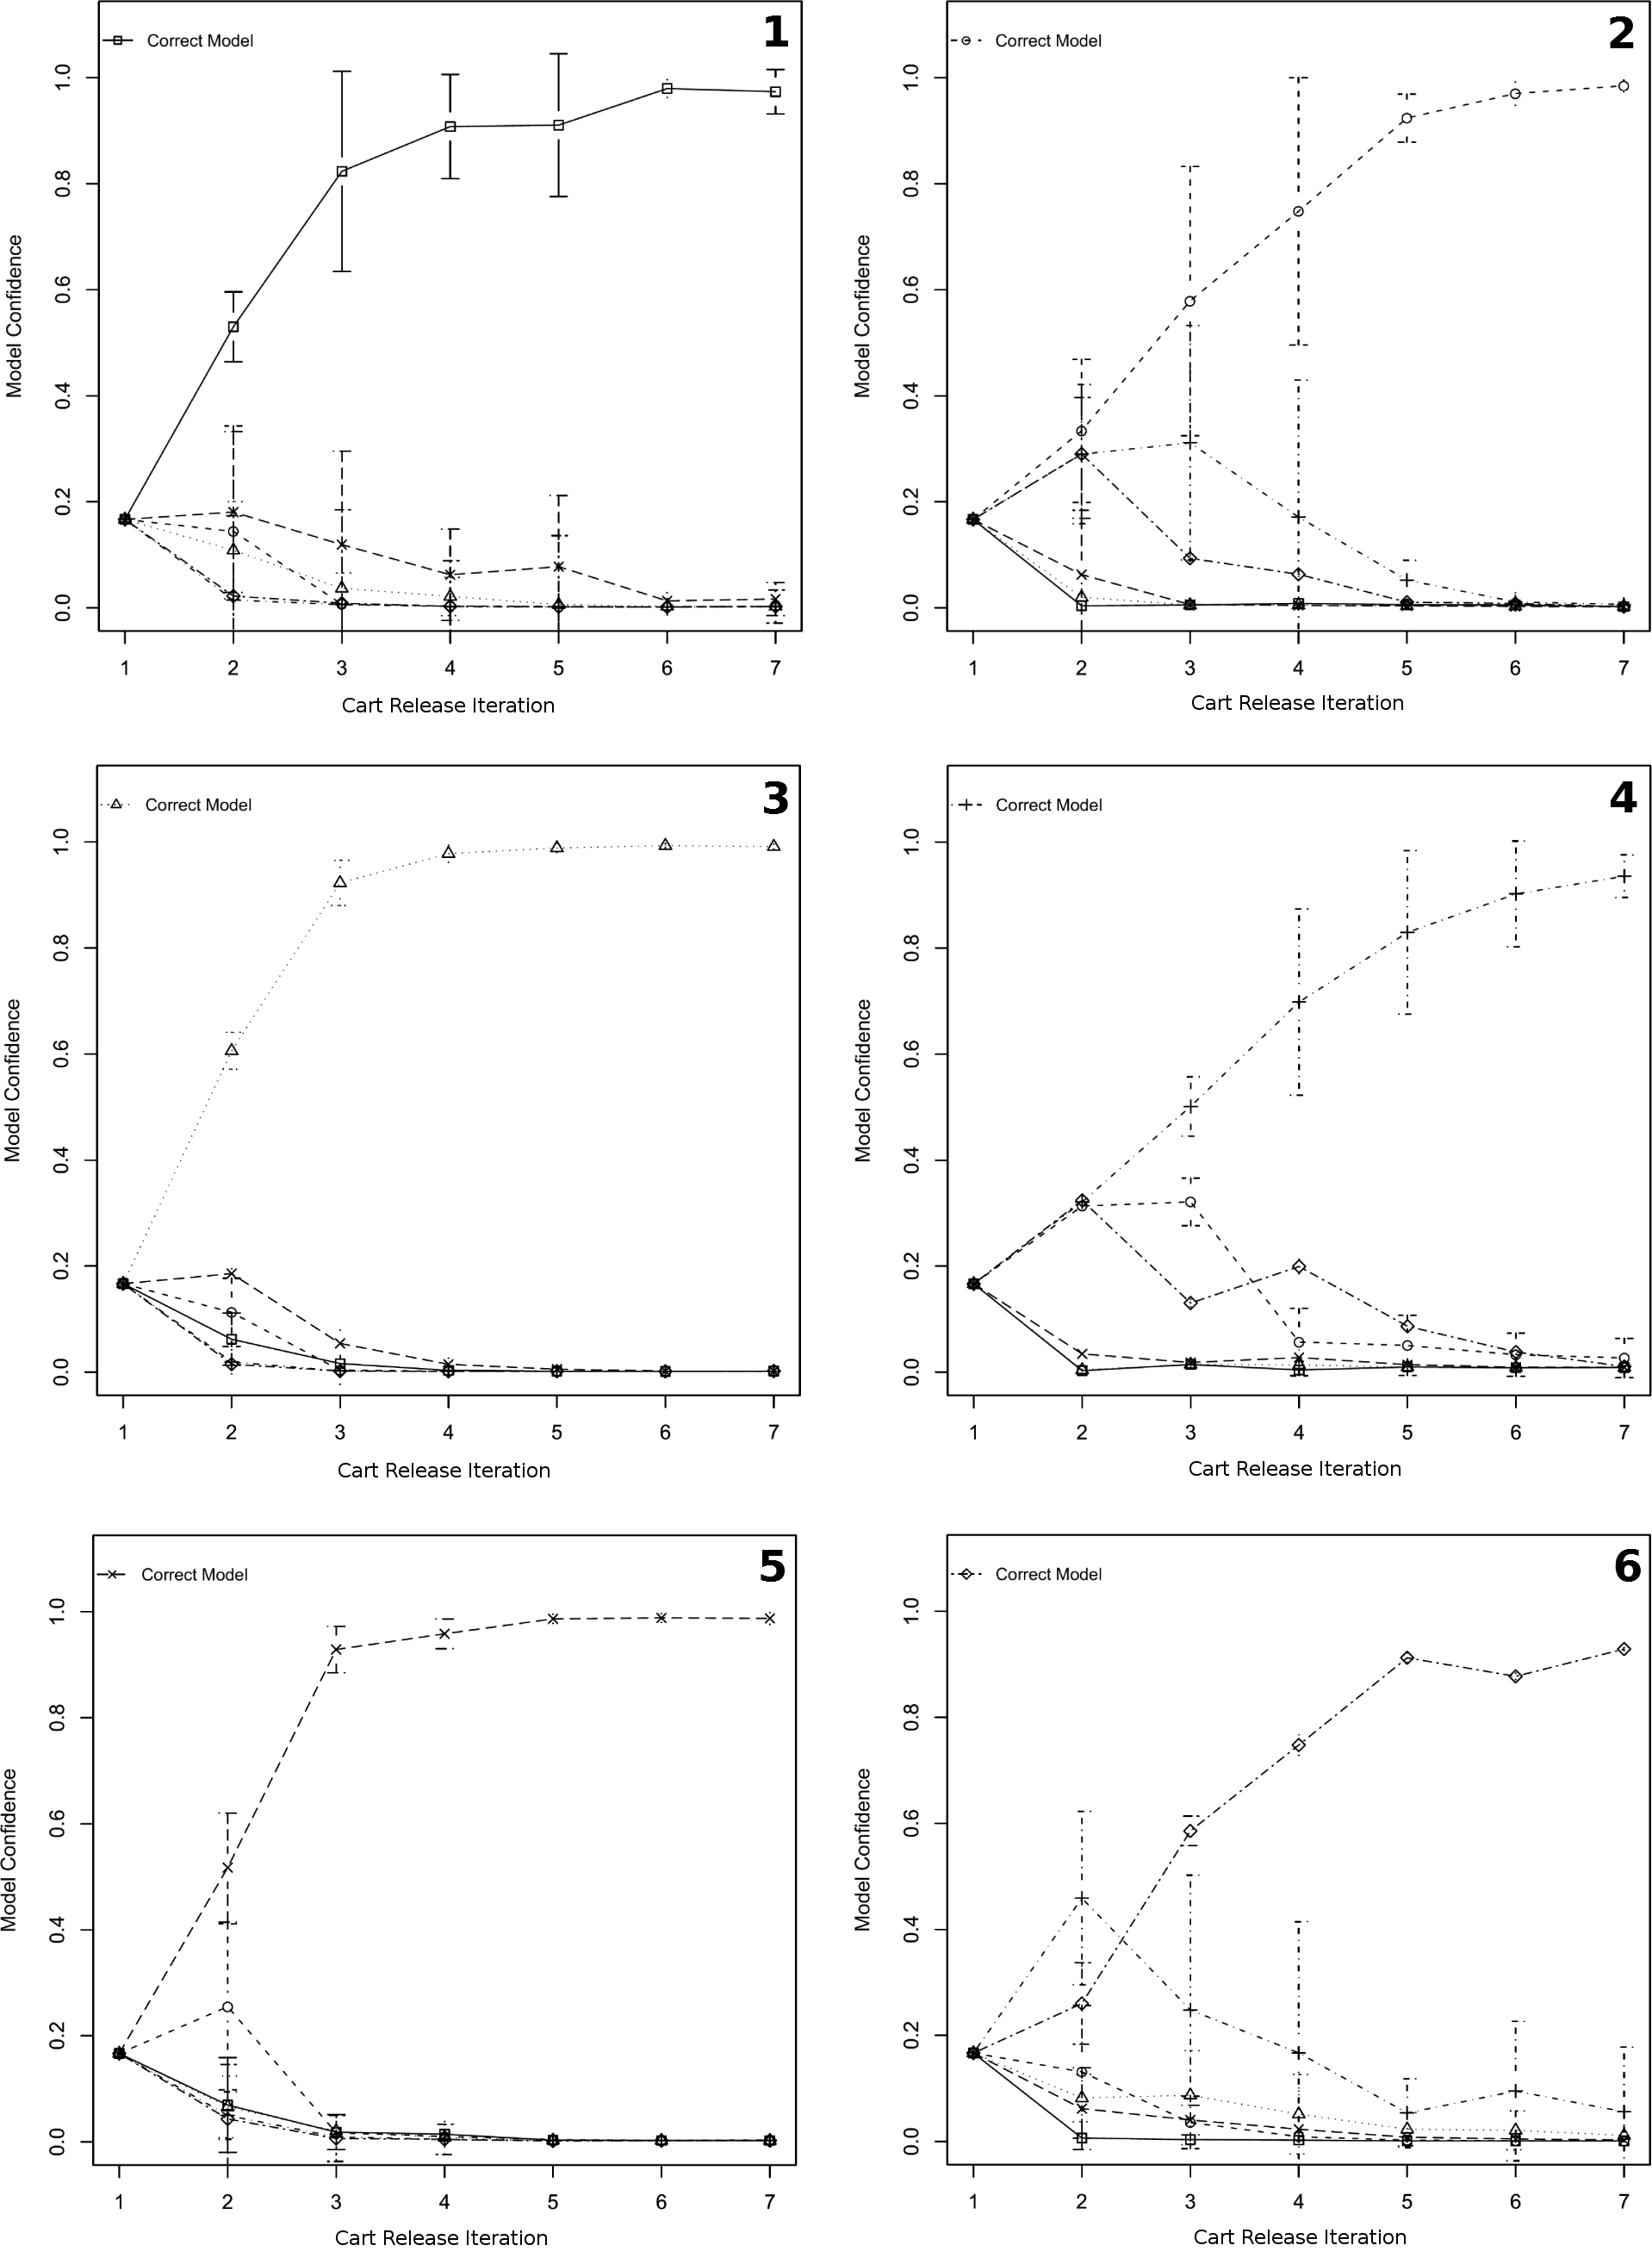
\includegraphics[width=1\textwidth]{images/roll}
\par\end{centering}

\caption{The results of the \emph{Wheel Configuration Experiment} in terms
of the model confidence distribution after a number of release iterations.
The underlying configuration of the physical box-cart in each of the
above runs matches the corresponding configuration shown in Figure
\ref{fig:Wheels-experiment-models.}. The error bars signify the $95\%$
confidence interval. We label only the correct object model confidence
in each graph. This is the model corresponding to the true underlying
configuration of the box cart.\label{fig:Wheels-ramp-experiment.}}
\end{figure}


In additional to evaluating the performance of learning the configuration
of the box-cart object, we investigated the effect of choosing the
action with highest expected information gain on the learning rate.
We compare in simulation a robot learning the box-cart's wheel configuration
using the most informative action at every step, and using a random
action at every step. It is important to note that this is carried
out purely in simulation, the actions are simulated in the same manner
as when building the action model. For the best action and random
action selection policies, three simulated runs are performed, each
with nine actions performed. The progression of the confidence distribution
over the possible object models is show in Figure \ref{fig:cart-sim}.
It can be seen that by choosing the most informative action leads
to a much faster convergence of the confidence distribution to the
correct object model, whereas choosing a random action leads to much
worse performance.

\begin{figure}
\begin{centering}
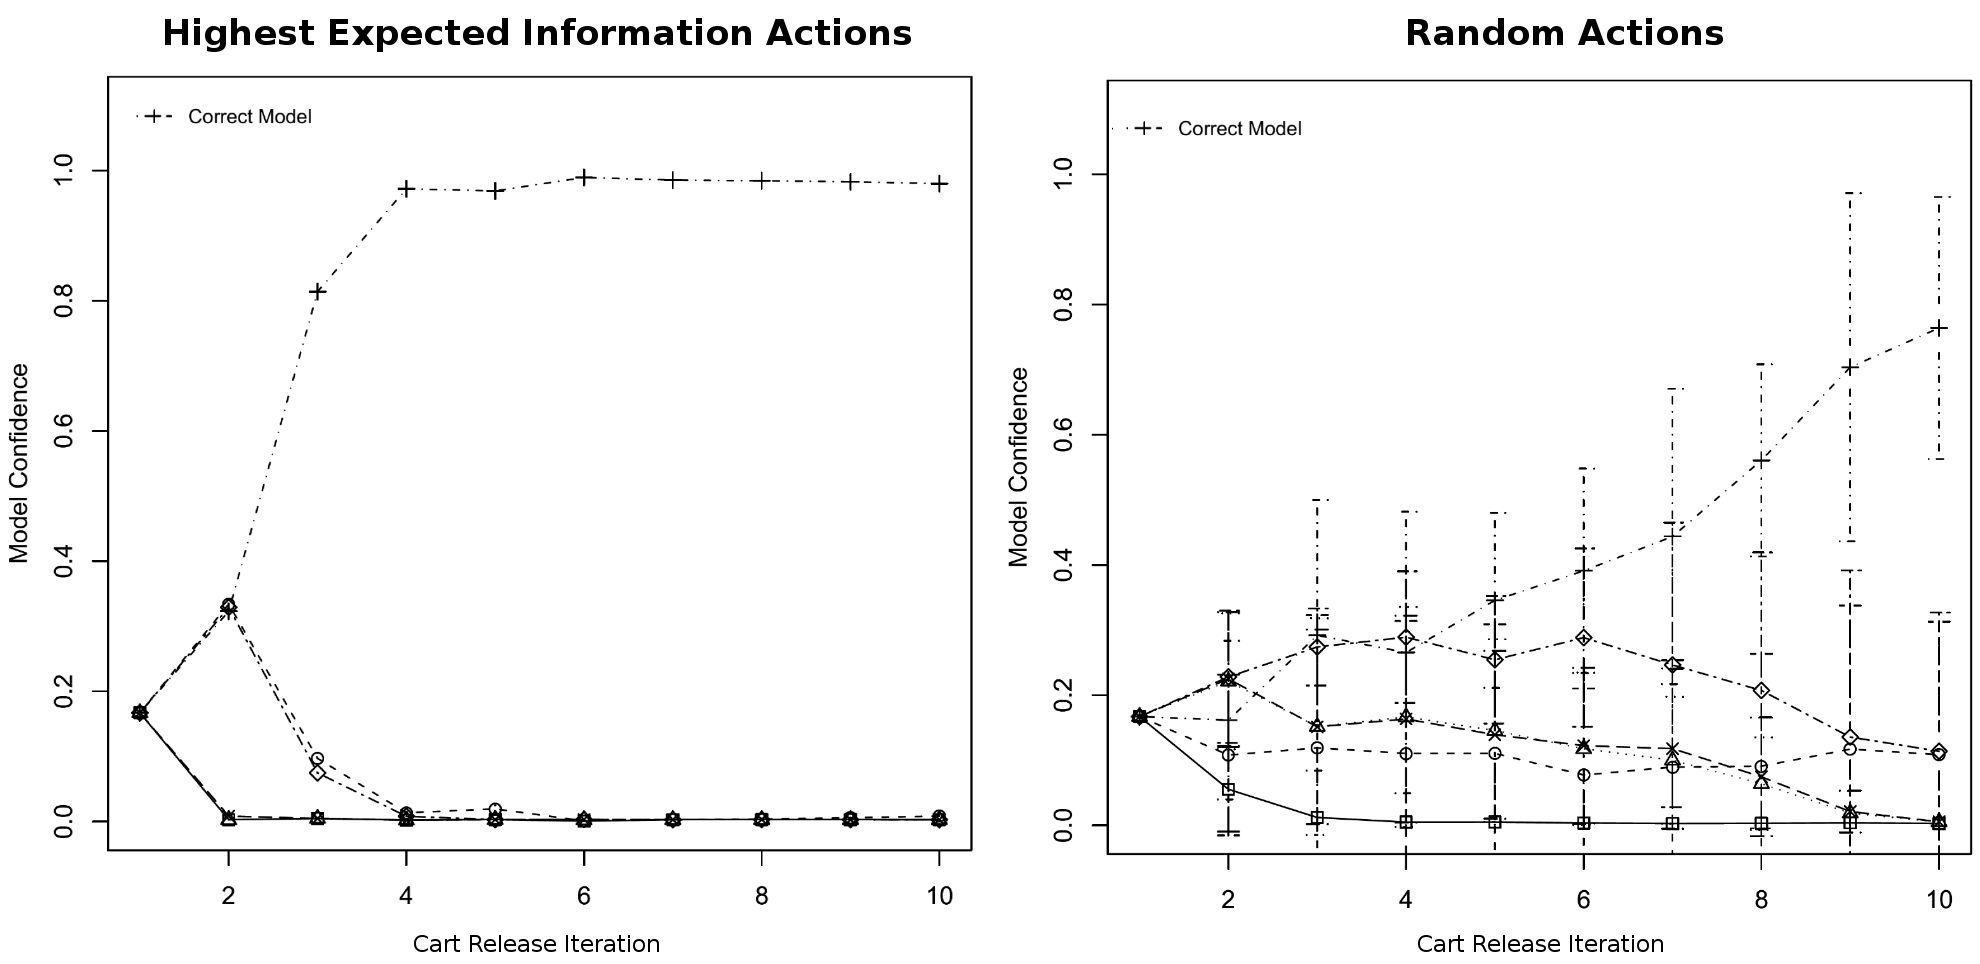
\includegraphics[width=1\textwidth]{images/roll_sim}
\par\end{centering}

\caption{Learning the box-cart wheel configuration using the action with highest
expected information gain (left), and using a random action (right)
at every iteration. This is performed in simulation with the simulated
box-cart having its wheels set to configuration 4 as seen in Figure
\ref{fig:Wheels-experiment-models.}. By performing the most informative
action the confidence distribution quickly converges on the correct
object model. When performing a random action, the confidence distribution
on average does not reliably converge. The error bars indicate the
$95\%$ confidence interval.\label{fig:cart-sim}}
\end{figure}



\subsection{Stimulus Response Behaviour Experiment\label{sub:Stimulus-Response-Behaviour}}


\subsubsection*{Overview}

In this experiment we demonstrate that the general active learning
framework is applicable to a wide variety of object properties. In
this case the robot determines a behavioural model of an object, rather
than a physical property. The object in question is a Lego Mindstorms
bot which is programmed to respond to light stimuli. The Lego-bot
is composed of two motor driven wheels, and two light sensors (see
Figure \ref{fig:Lego-Mindstorms-robot.}). It is programmed to perform
a certain movement behaviour if one of its sensors is stimulated by
light. A sensor is said to be stimulated if it detects a high light
level as compared to the other sensor. An example movement behaviour
is turn left $45\textdegree$ and move forward $15cm$ if the left
light sensor is stimulated. 

\begin{figure}
\begin{centering}
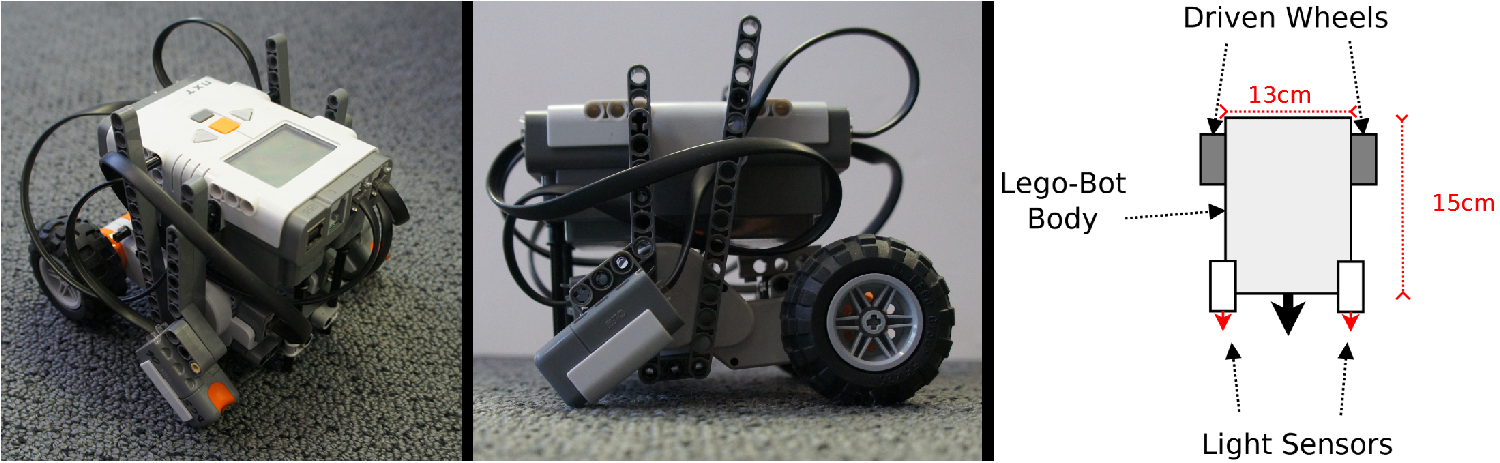
\includegraphics[width=1\textwidth]{images/lego_img}
\par\end{centering}

\caption{Lego Mindstorms robot. It is composed of the NXT Intelligent brick,
two motor driven rear wheels, and two light sensors. The light sensorrs
are facing forward and downward at a $45\textdegree$ angle.\label{fig:Lego-Mindstorms-robot.}}
\end{figure}


The task of the main robot is to perform some actions to determine
a model which matches the Lego-bot's movement behaviour. For this
purpose a flashlight is attached to the gripper, which the robot can
then use to project light onto the workspace. This is illustrated
in Figure \ref{fig:Light-sensing-bot}. The robot can perform actions
in the form of shining the flashlight onto particular areas of the
workspace, and observing the resultant Lego bot's motion. This motion
provides information as to the bot's underlying programmed behaviour.
A simulator is used in order to predict the outcome of the various
possible actions on the possible object models in order to choose
the most informative action.

\begin{figure}
\begin{centering}
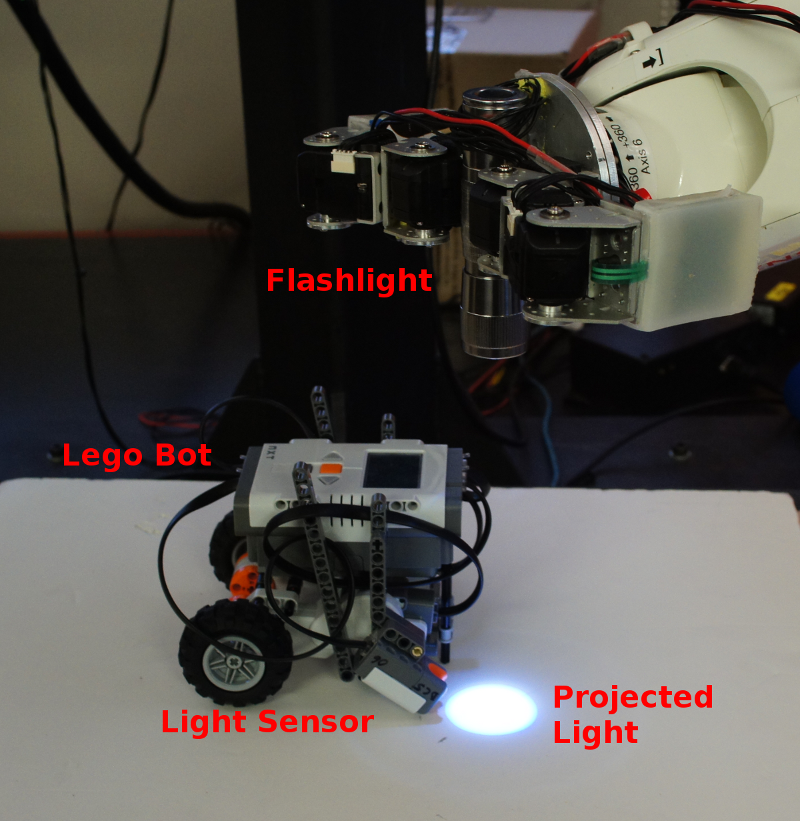
\includegraphics[width=0.6\textwidth]{images/light}
\par\end{centering}

\caption{The robot uses a flashlight attached to the gripper in order to perform
illumination actions to determine the light stimulation response behaviour
of the Lego Mindstorms bot. An action is in the form of shining the
flashlight onto the workspace to stimulate the light sensors on the
Lego bot.\label{fig:Light-sensing-bot}}
\end{figure}


The procedure followed by the robot in this experiment differs from
the previous two experiments in that the robot does not directly manipulate
the target object. Instead the robot uses a flashlight attached to
its gripper to illuminate the workspace and trigger the Lego bot's
movement behaviour. To learn the object model the robot performs the
following steps:
\begin{enumerate}
\item Localise the Lego bot in the scene;
\item Calculate the information gain of each action given the current model
likelyhood distribution;
\item Carry out the most informative action possible by illuminating the
appropriate part of the workspace with the flashlight;
\item Determine the resulting pose of the Lego bot;
\item Classify the resulting pose by matching it to a result label;
\item Update the model likelyhood distribution using the outcome probabilities
of the performed action and the result label.
\end{enumerate}
The cart is localised in a scene using the method described in previous
chapter, using a complete aspect graph of SIFT features and a depth
camera. Grasping is performed along the longest axis of the top of
the cart, with the vector between the two gripper pads parallel to
the ground plane.

In the remainder of this section we present the following: the possible
models that can describe the movement behaviour of the Lego bot and
the actions that the robot can perform (Section \ref{sub:Object-Models-and2}),
the simulation method used to determine the action probability models
(Section \ref{sub:Simulation-Method2}), the method of labeling the
result of each action with a discrete label (Section \ref{sub:Result-Classification2}),
and the performance results of determining the behaviour model of
the Lego cart using the active object model learning approach (Section
\ref{sub:Performance-Results2}).


\subsubsection{Possible Object Models and Actions\label{sub:Object-Models-and2}}

The robot's task is to determine the underlying movement behaviour
of the Lego bot. This is done by finding a model from a predefined
set of possible object models which best fits the observed results
of performed actions. For this experiment the set of potential models
that may describe the Lego bot's behaviour is of size 16. If the left
sensor is stimulated, the bot may turn $0\textdegree$ or $45\textdegree$
left, followed by moving forward $0cm$ or $15cm$. If the right sensor
is stimulated, the bot may turn $0\textdegree$ or $45\textdegree$
right, followed by moving forward $0cm$ or $15cm$. A sensor is said
to be stimulated when its sensed light level exceeds the sensed light
level of the opposing sensor by $1.5\times$.

The robot determines which of the potential models most accurately
matches the behaviour of the Lego bot by performing actions from an
available pool and observing the results. The robot gripper has a
flashlight attached which emits a focused light cone measured to have
a $15.3\textdegree$ spread. The robot moves the gripper into a particular
position to shine the light onto the Lego bot. Each illumination action
can be defined by three parameters, the $(x,y)$ position of the light
cone relative to the Lego bot, and the height of the light above the
table surface. The height determines the size of the projected light
circle on the table surface. We predefine an \emph{ad hoc} pool of
$250$ possible actions, generated by randomly choosing $50$ $(x,y)$
positions falling inside a circle of radius $15cm$ from the centre
of the Lego bot, and for each position the height of the light above
the table top may be one of the following $5$ values $\left\{ 20cm,25cm,30cm,35cm,40cm\right\} $. 


\subsubsection{Simulation Method\label{sub:Simulation-Method2}}

In order to determine the probability distribution over results of
each action on the potential models we use a simulation method. However,
unlike with the \emph{Centre of Mass} and \emph{Wheel Configuration}
experiments, there are no convenient physics engine primitives for
simulating a Lego Mindstorms robot programmed with a certain behaviour.
Instead we must explicitly approximate the amount of light sensed
by a light sensor when the flash light is placed in a given position
relative to the Lego bot. This is followed by simulating the movement
performed by the Lego bot if the light response behaviour is triggered.

We simulate the flash light by computing the circle of light it projects
onto the table surface from a given position. The flash light is held
vertical in all cases, and the beam spread is known to be $15.3\textdegree$.
This allows us to compute the light circle's position and size for
any given illumination action, where each is specified by the relative
position and height of the flash light to the Lego bot. We then compute
how much of this projected light circle falls within the field of
view of the light sensor. We do this by projecting a large number
of rays from the position of each light sensor. These rays are projected
in a cone of angle $45\textdegree$ with the axis oriented in the
direction of the light sensor (at a $45\textdegree$ angle looking
at the ground). Each of these sample rays are intersected with the
ground plane The percentage of all of the sampling rays of a light
sensor that have their ground intersection point fall within the projected
light circle is said to be the light value sensed by the sensor. Figure
\ref{fig:lego-sim} illustrates the ray casting method. We do this
for both the left and right light sensors, and compare the computed
values. If the computed value of one of the sensors is more than $1.5\times$
that of the other, the model movement behaviour is triggered. To simulate
a movement behaviour, we simple rotate and translate the simulated
Lego bot object as dictated by the particular behaviour model.

\begin{figure}
\begin{centering}
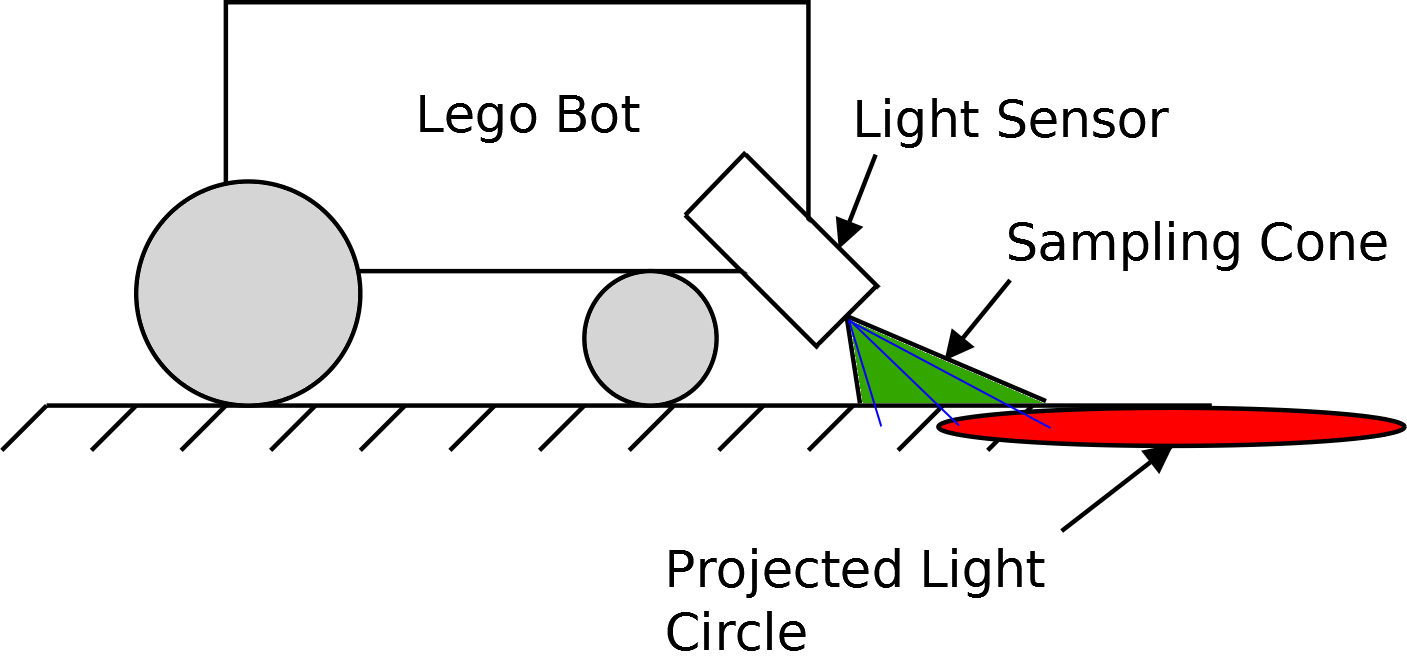
\includegraphics[width=0.8\textwidth]{images/lego_light_compute}
\par\end{centering}

\caption{This diagram shows how we simulate the amount of light sensed by a
light sensor when the flashlight casts a light circle on the ground.
We project multiple rays (denoted by blue lines inside the sampling
cone) from the light sensor's position, in a sampling cone of angle
$45\textdegree$ in the direction the sensor is pointing. The percentage
of these light rays that intersect the projected light circle is taken
as the light sensed by the sensor. This value can then be compared
to the light sensed by the opposing sensor to determine if the Lego
bot's movement behaviour is triggered.\label{fig:lego-sim}}
\end{figure}


In order to account for various sources of error and noise when the
illumination action is performed in real life, we apply a noise model
to each simulated run. This is done by perturbing the light circle's
size and position, as well as the amount the simulated Lego-bot turns
and drives forward, using Gaussian noise. The light circle position
is shifted in a random direction on the $xy$ plane by noise with
standard deviation $0.5cm$ and mean $0cm$. The light circle size
perturbation has a standard deviation of $0.5cm$ and mean $0cm$.
When the simulated Lego-bot turns, the turn amount perturbation has
a standard deviation of $10\textdegree$ and mean $0cm$, when it
drives forward the perturbation for the distance driven has a standard
deviation of $1cm$ and mean $0cm$. These perturbations are chosen
\emph{ad hoc}, but are set to overestimate the actual error in the
Lego bot's movement.


\subsubsection{Result Classification\label{sub:Result-Classification2}}

The result labels are generated by discretising the workspace into
uniform cells, followed by matching the Lego-bot's resulting pose
at the conclusion of an action iteration to one of these cells. The
discretisation is achieved by dividing a square $50cm\times50cm$
centered on the Lego-bot into $100$ $5cm\times5cm$ cells. In order
to discretise the orientation, each of these is further divided into
$24$ orientation cells, dividing the $360\textdegree$ circle into
$15\textdegree$ increments. The end result is $2400$ possible result
labels. 

When an illumination action is performed, to determine the outcome
result label, we first calculate the relative motion of the Lego-bot
to its starting pose. From this relative pose we then calculate $(x,y,\theta)$,
which is the relative amount the robot moved on the $(x,y)$ plane
and the angle amount it has rotated around the vertical axis. This
relative pose is then matched to one of the $2400$ possible result
label cells.


\subsubsection{Performance Results\label{sub:Performance-Results2}}

We test the performance of the learning system by having the robot
carry out multiple runs of learning the behaviour model of the Lego
bot. In each run the robot performs a series of actions, updating
the confidence distribution over the possible models using the result
of each action.

To test the effectivenes of our approach we used three different scenarios
(the Lego bot was programmed with three different behaviours), for
each scenario the robot performed three independent runs of the learning
algorithm, each run involved a series of 6 illumination actions in
order to determine the underlying model of the Lego bot's behaviour.
In the first scenario the Lego bot is programmed to not move at all,
that is, to not respond to stimuli. In the second scenario the Lego
bot is programmed to turn left when the left sensor is stimulated,
otherwise to remain stationary. In the third scenario the Lego bot
is programmed to turn left and move forward when the left sensor is
stimulated, and move forward without rotating when the right sensor
is stimulated. The results are presented in Figure \ref{fig:Lego-experiment-results.}
and show how the robot's confidence distribution over the 16 possible
behaviour models changes during the course of each iteration. We can
see that the robot's confidence distribution quickly tends toward
the correct model describing the Lego bot's behaviour in all 3 instances.

\begin{figure}
\begin{centering}
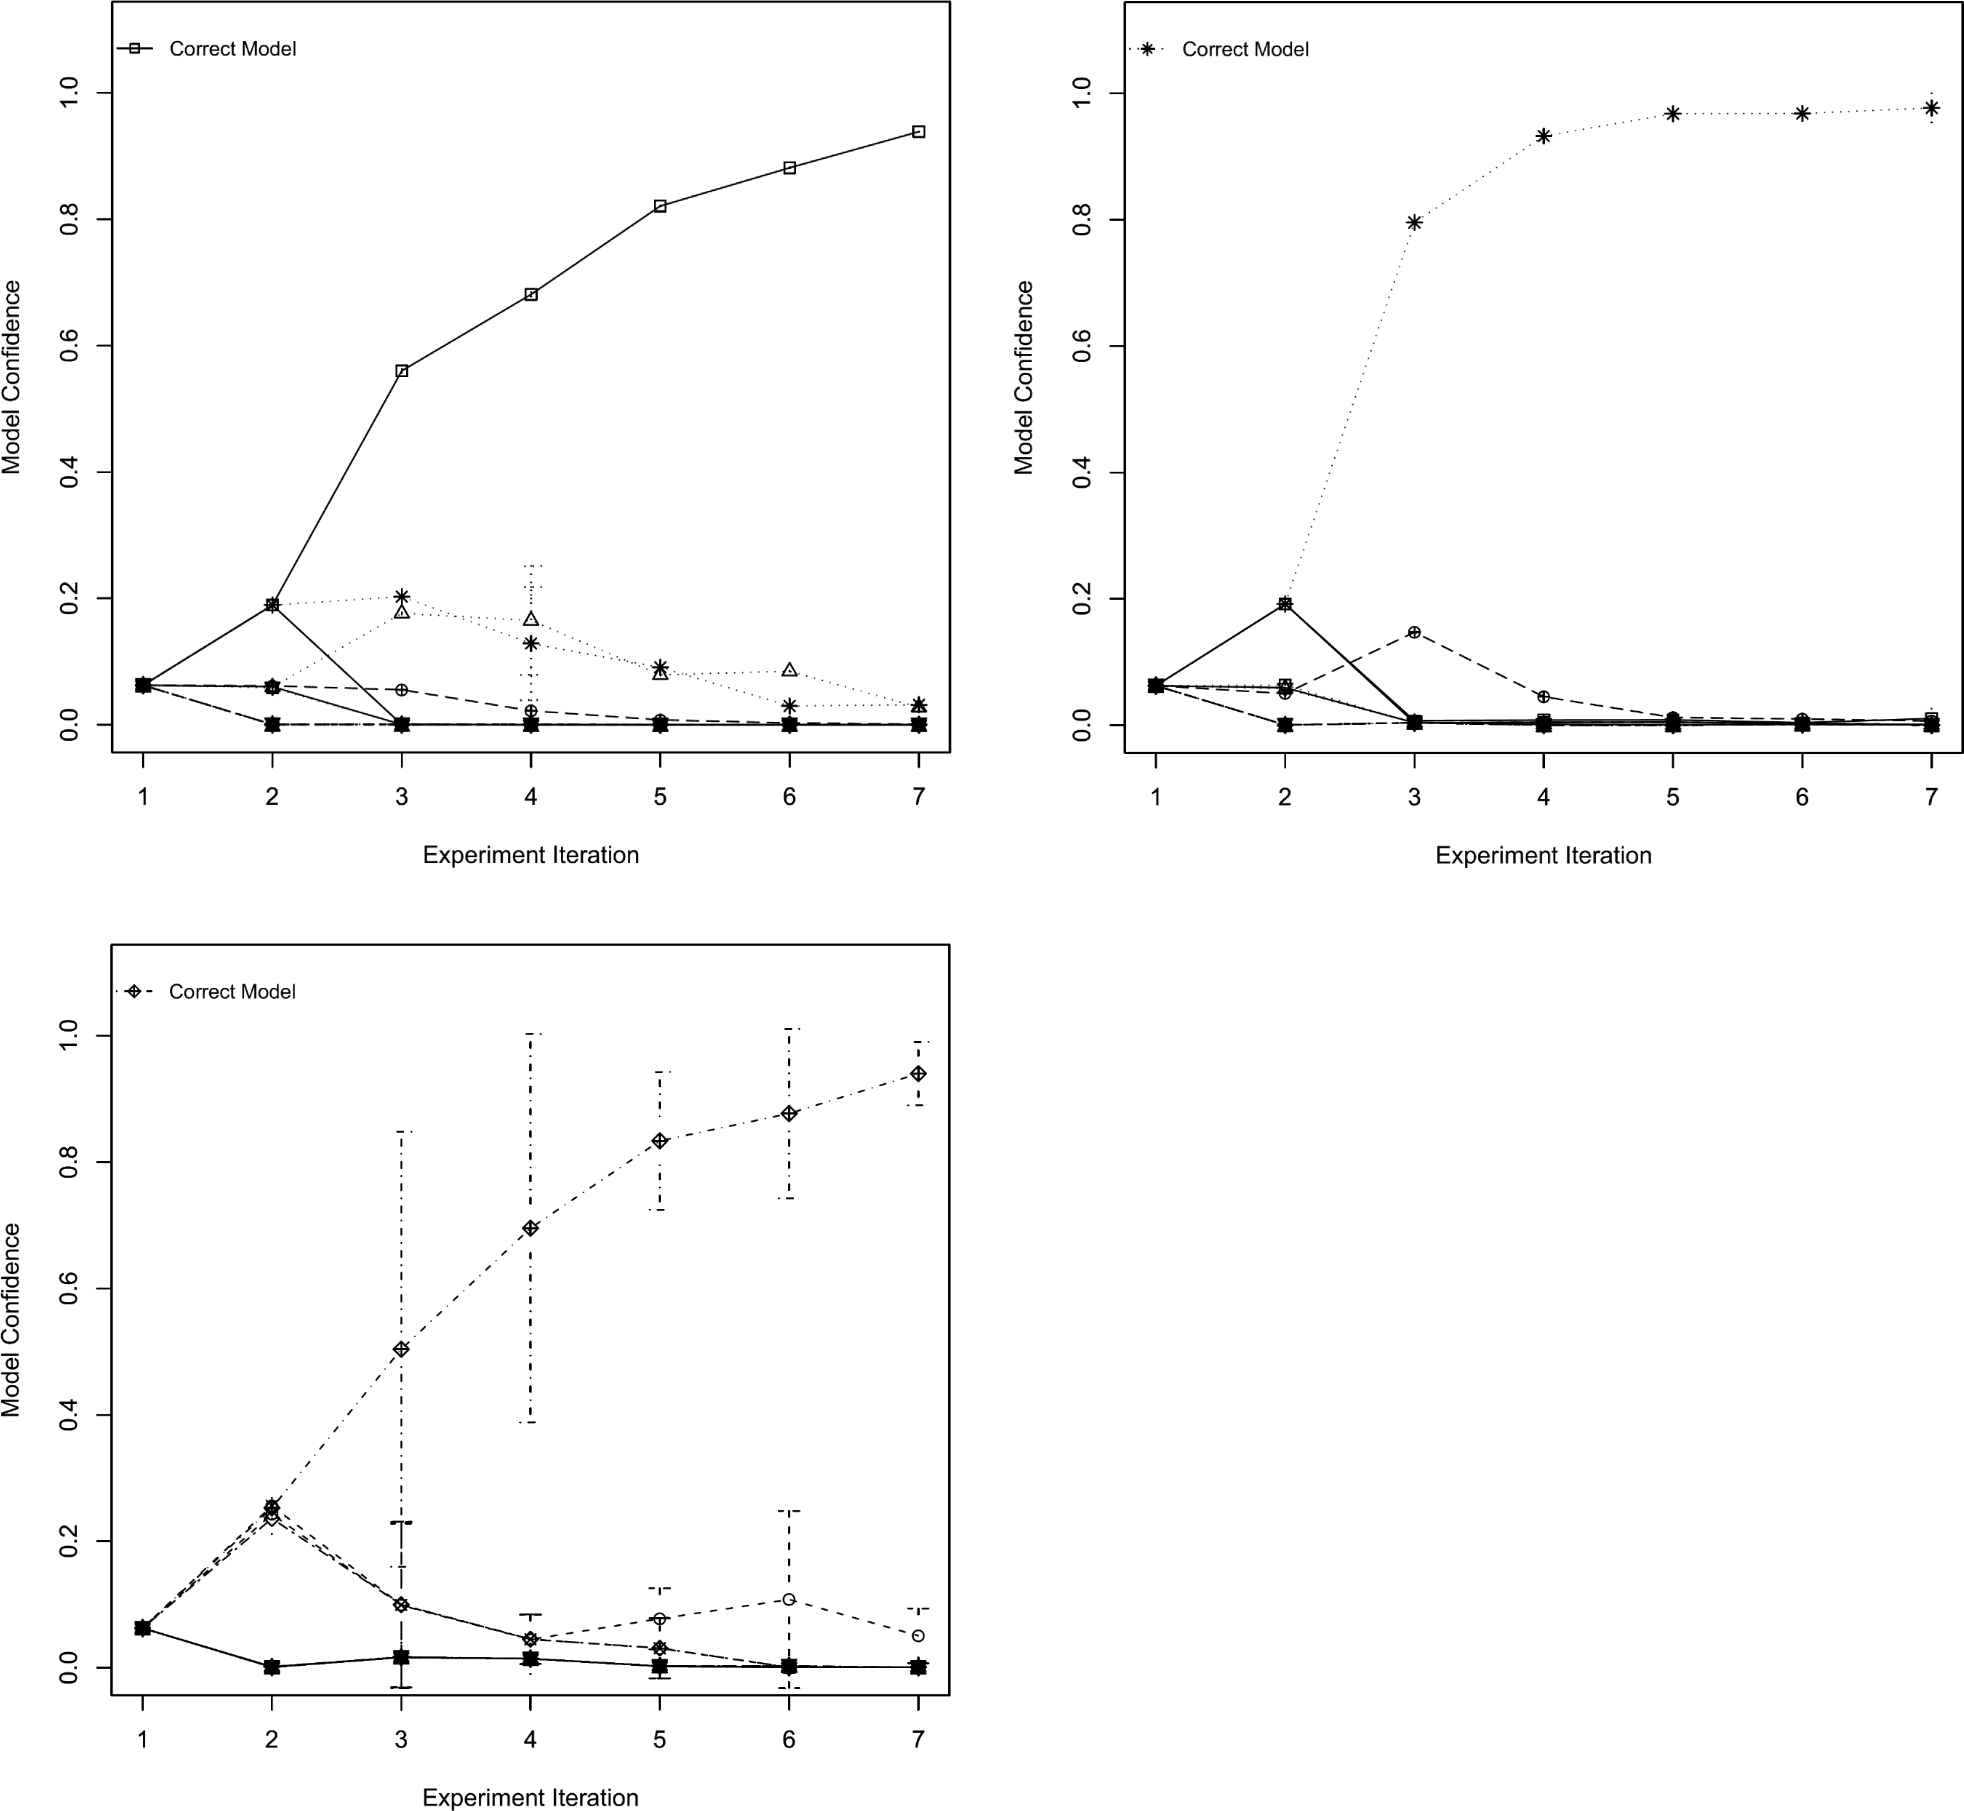
\includegraphics[width=1\textwidth]{images/lego}
\par\end{centering}

\caption{The results of the \emph{Stimulus Response Experiment} showing the
progression of the model confidence distribution after a number of
illumination action iterations. There are 16 possible models that
can describe the Lego bot behaviour, the above results show how the
robot's confidence distribution over the potential models evolved
when performing actions in 3 different scenarios. Top Left corresponds
to a scenario in which the Lego bot does not respond in any way to
light. Top Right corresponds to the scenario in which the Lego bot
is programmed to turn left when the left sensor is stimulated. The
Bottom Left corresponds to the scenario in which the Lego bot is programmed
to turn left and move forward when the left sensor is stimulated,
and move forward when the right sensor is stimulated. The error bars
correspond to the standard deviation across 3 trials for each scenario.
We omit individually labeling each line in the graphs as there are
16 different models. We only provide a label for the correct model
confidence in each instance.\label{fig:Lego-experiment-results.}}
\end{figure}


In additional to evaluating the performance of the object model learning
method, we investigated the effect of choosing the action with highest
expected information gain on the learning rate. We compare in simulation
a robot learning the Lego bot's behaviour using the most informative
action at every step, and using a random action at every step. The
actions are simulated in the same manner as when building the action
model. For the best and random action selection policies, three simulated
runs are performed, each with six actions performed. The progression
of the confidence distribution over the possible Lego bot behaviour
models is show in Figure \ref{fig:lego-sim-comp}. It can be seen
that by choosing the most informative action leads to a convergence
of the confidence distribution to the correct object model, whereas
choosing a random action does not result in a convergence on the correct
model. This is due to the fact that many of the possible actions do
not result in any response by the Lego bot. If neither of the light
sensors are illuminated by the flashlight, then the Lego bot's behaviour
will not be triggered and no information will be gained as a result.

\begin{figure}
\begin{centering}
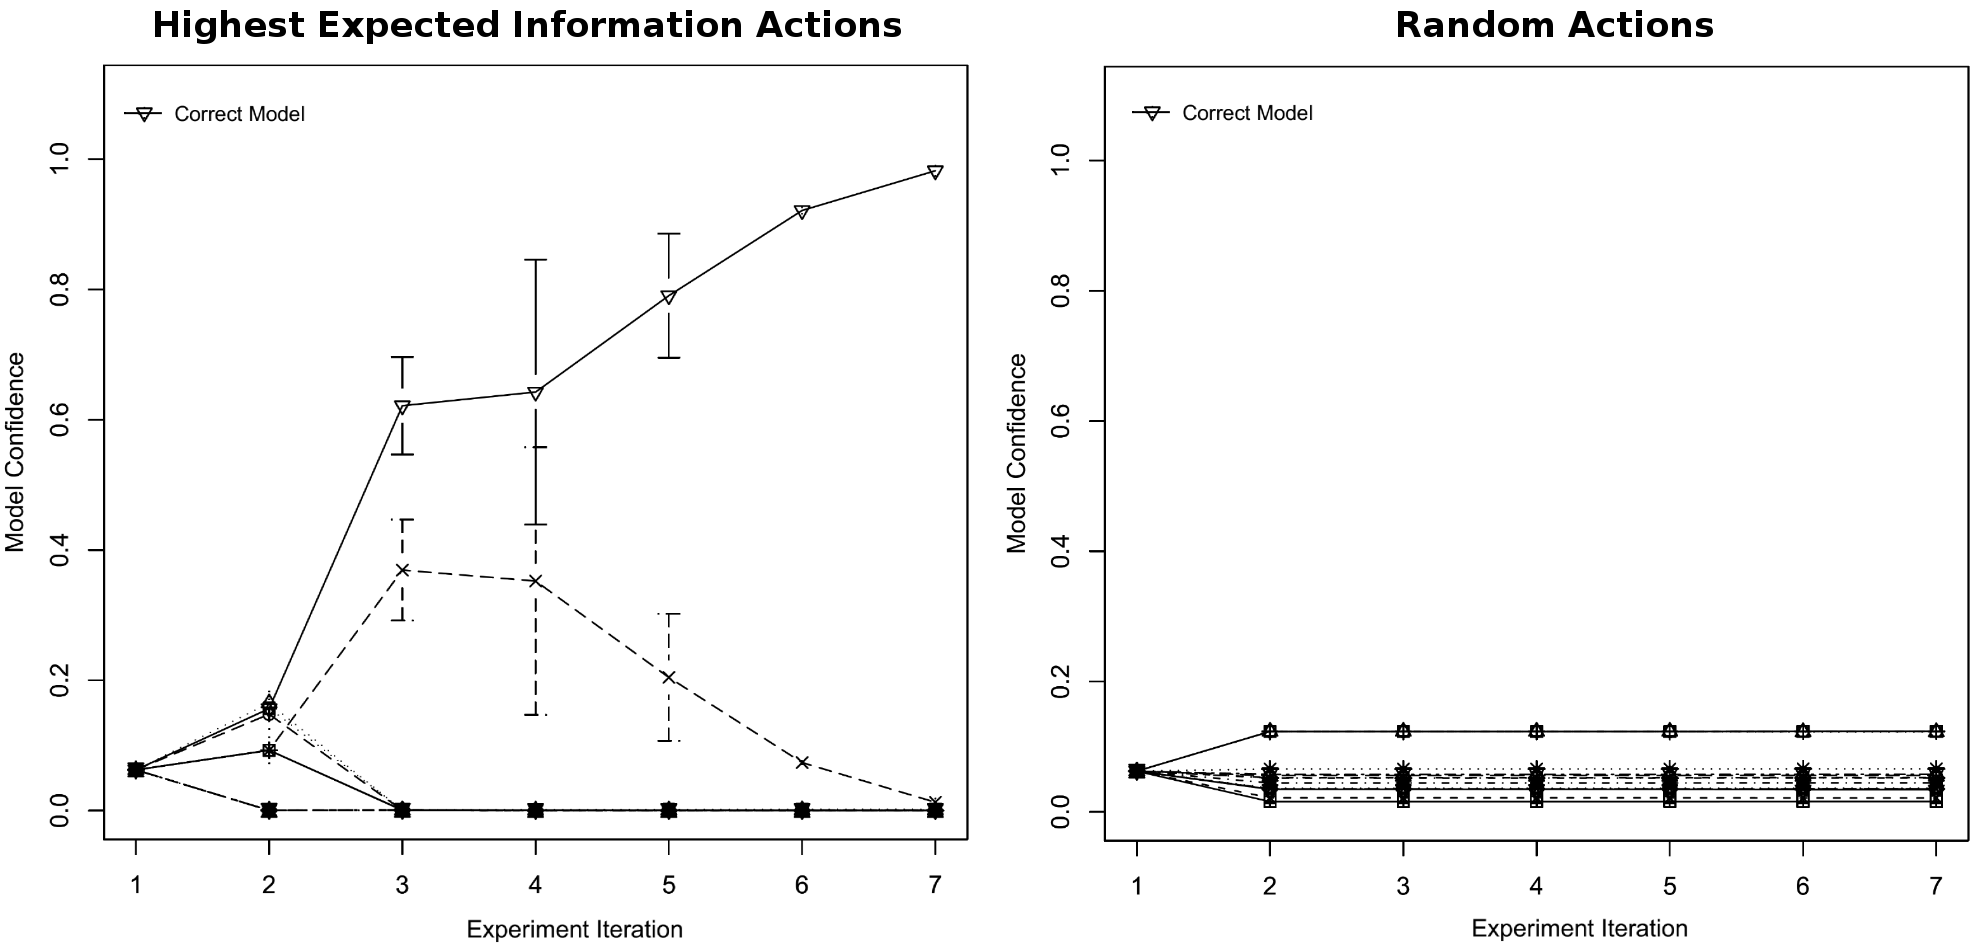
\includegraphics[width=1\textwidth]{images/lego_sim}
\par\end{centering}

\caption{Learning the Lego bot's behaviour using the action with highest expected
information gain (left), and using a random action (right) at every
iteration. This is performed in simulation with the simulated Lego
bot programmed to drive forward if its left sensor is stimulated,
and turn left and drive forward if its right sensor is stimulated.
By performing the most informative action the confidence distribution
quickly converges on the correct object model. When performing a random
action, the confidence distribution on average does not converge.
The error bars indicate the $95\%$ confidence interval.\label{fig:lego-sim-comp}}


\end{figure}



\section{Learned Model Exploitation\label{sec:Learned-Model-Exploitation}}


\subsubsection*{Overview}

The final experiment involves the robot performing a basic tool use
task using an object for which it has previously learned a physics
model. This learned model allows the robot to plan a solution to a
task using the predictive qualities of the model, and then carry out
the plan to complete the task.

The task goal for the robot is to knock over a cylinder standing vertically
in one of two possible positions on a flat surface. This cylinder
is out of reach of the robot arm, instead the robot must use a ramp
and a box-cart in order to knock down the cylinder by placing and
releasing the cart on the ramp in the appropriate orientation such
that its trajectory intersects the position of the cylinder. The workspace
consists of a flat table top and a $20\textdegree$ ramp. The cylinder
is placed upright on the flat table top in one of two positions, 15cm
and 20cm from the end of the ramp. This configuration is shown in
Figure \ref{fig:The-workspace-layout}.

\begin{figure}
\begin{centering}
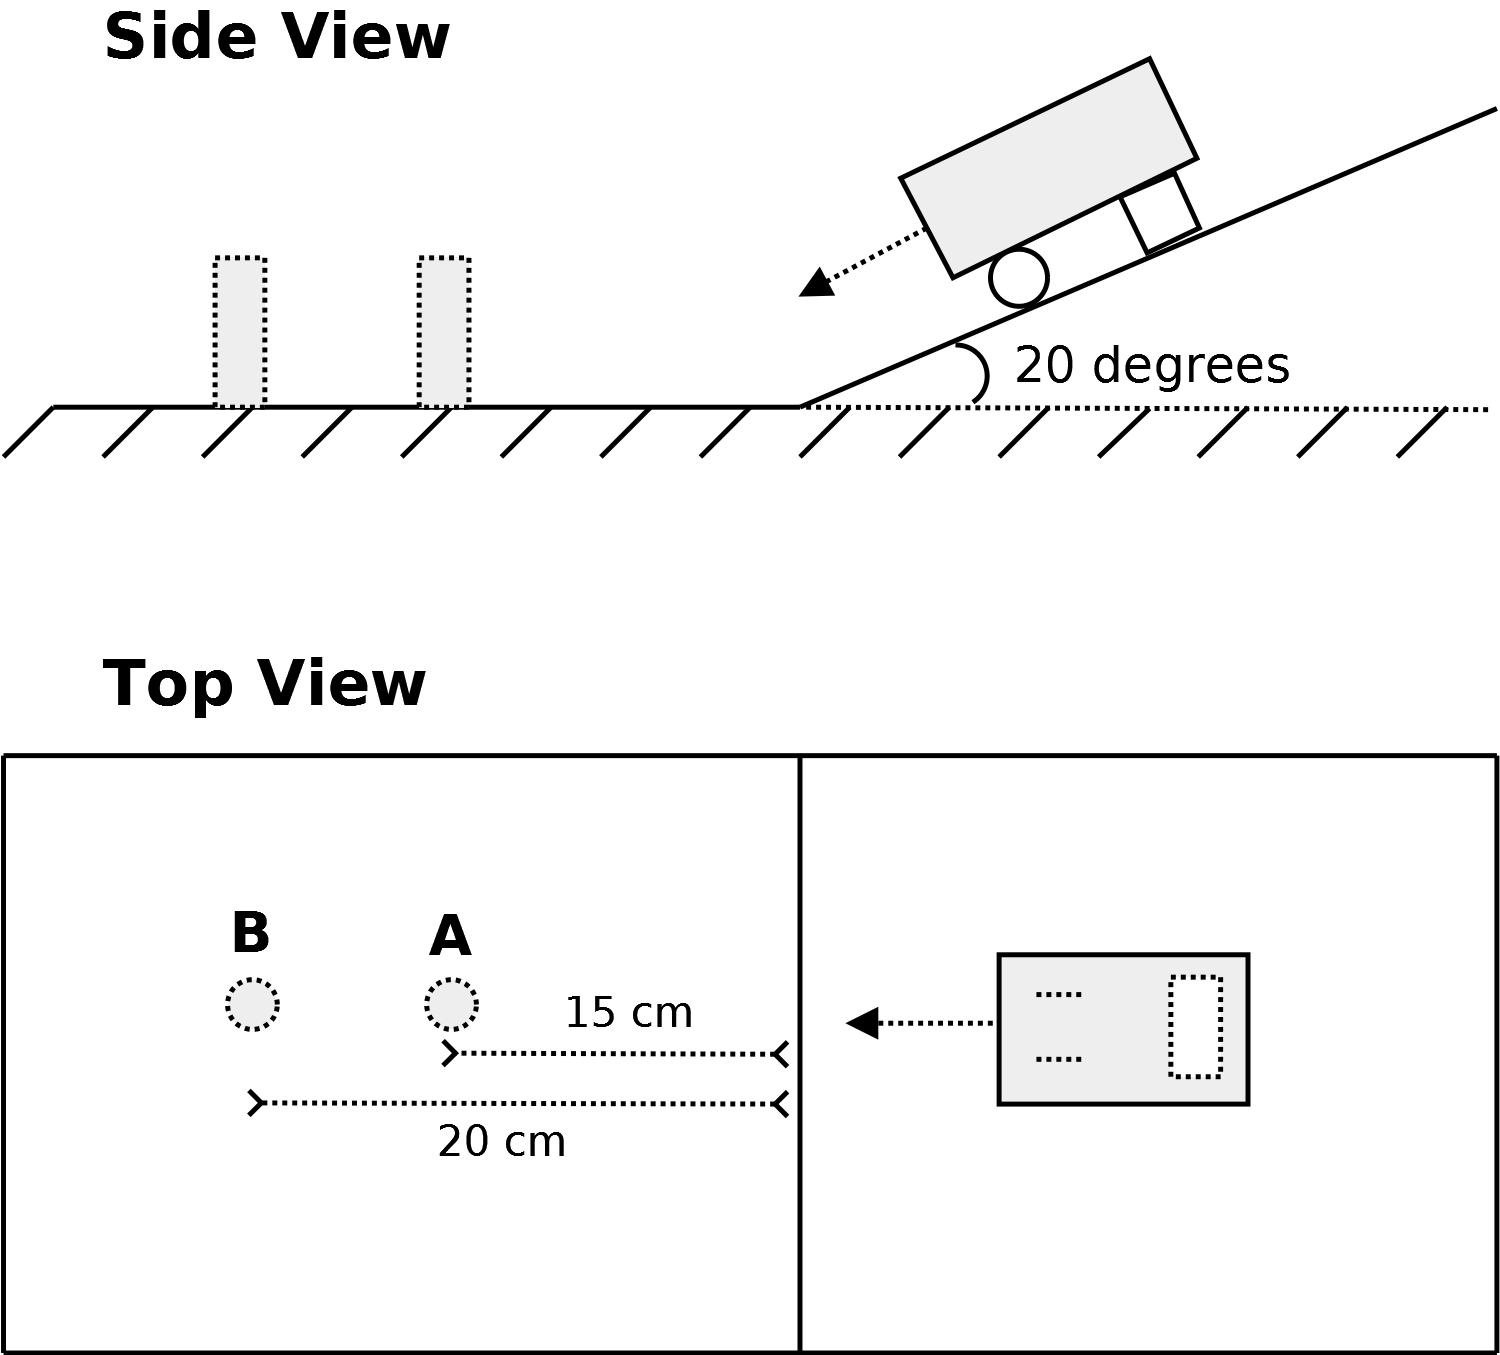
\includegraphics[width=0.7\textwidth]{images/knock_experiment}
\par\end{centering}

\caption{The above figure represents the workspace layout for the \noun{Tool
Use} task. In this task the robot has a similar workspace to the \emph{Wheels
Experiment}, but with the addition of a peg placed at one of two possible
positions\emph{, A} and \emph{B} ($15cm$ and $20cm$ from the ramp),
the ramp angle is set to $20\textdegree$. The robot's task is to
use the internal simulated model of the box-cart object (which was
determined in the \emph{Wheels Experiment}) to release the cart from
an appropriate position and orientation on the ramp to knock down
the peg.\label{fig:The-workspace-layout}}
\end{figure}


The wheels of the box-cart can either be directed forward, or at a
$45\textdegree$ angle to the left, both wheels are free to rotate
on the axle. These two possible cart configurations are illustrated
in Figure \ref{fig:Possible-box-cart-wheel}. The robot has a learned
physics engine model of this box-cart, which is determined using the
method from Subsection \ref{sub:Wheels-Experiment} (note that the
ramp angle during learning is $25\textdegree$, whereas during this
task it is $20\textdegree$). The robot uses this model to simulate
the outcome of releasing the box-cart from many different poses on
the ramp. It chooses the best release pose, and performs the corresponding
action on the real world box-cart in order to knock down the cylinder.
The purpose of this experiment is to demonstrate the feasibility of
using a predictive object model in the form of a physics engine to
plan a solution to a task, the importance of learning the correct
object model, and the ability to use a learned physics model to make
predictions in an environment different to that during learning.

\begin{figure}
\begin{centering}
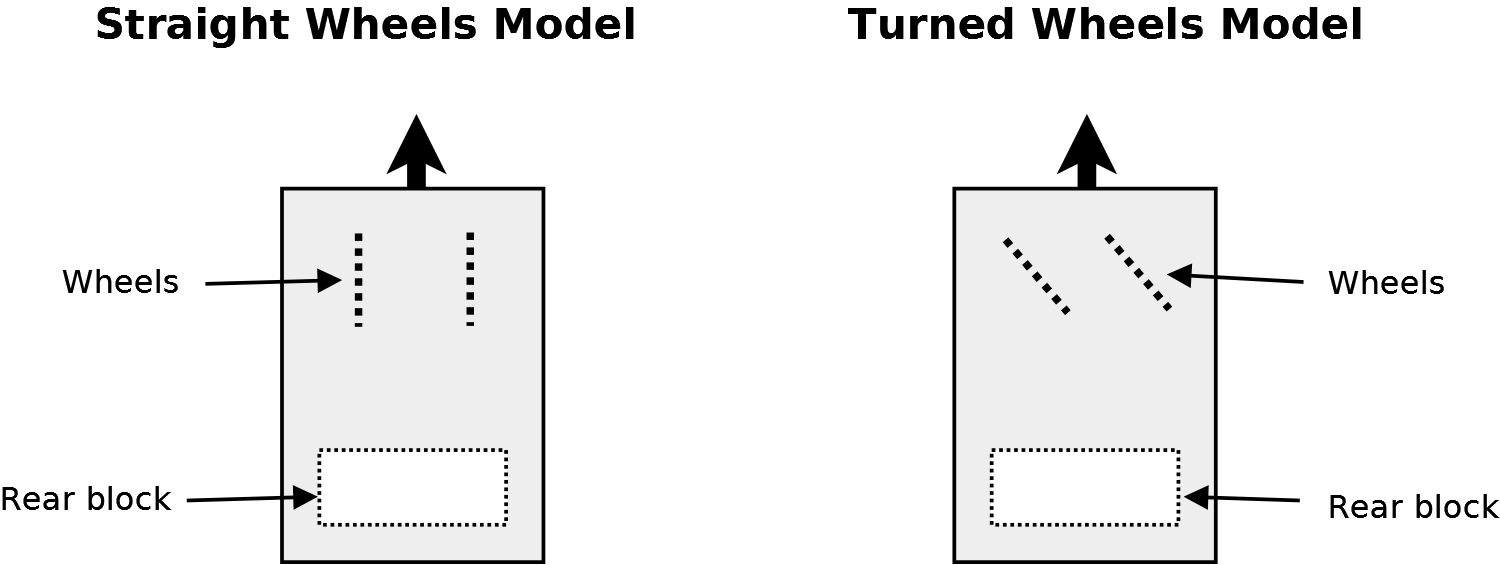
\includegraphics[width=0.8\textwidth]{images/wheels_knock_models}
\par\end{centering}

\caption{Possible box-cart wheel configurations models. The wheels of the box-cart
can either be oriented straight ahead, or at a $45\textdegree$ angle
to the left. Box wheels are free to rotate.\label{fig:Possible-box-cart-wheel}}
\end{figure}


To find the release pose for the box-cart with the best chance of
knocking over the cylinder, the robot performs a non-linear numerical
optimisation over the release pose parameter space. We use the Nelder
Mead optimisation method, as it is simple to implement and this particular
problem has a low dimension and smooth parameter space. In principle
other optimisation methods, for example Simulated Annealing or Hill
Climbing, may be used instead. The value of the objective function
to be optimised is determined by performing a number of simulations
where the simulated box-cart model is released in the specified pose.
The simulation is run for 600 frames at a step rate of 30 frames per
second. For each simulated frame the position of the box-cart is recorded.
The output of a single simulation run is the smallest distance between
the box-cart and the position of the cylinder during the run. This
is performed multiple times in order to account for the noise in the
simulated action. The noise model used is identical to that in Subsection
\ref{sub:Wheels-Experiment}. The final output of the objective function
is the average smallest distance between the box-cart and the cylinder.
This objective function is summarised in Algorithm \ref{alg:Box-cart-positioning-objective}.
Using the Nelder Mead algorithm we find the box-cart release pose
which minimises this objective function. Finally, the robot picks
up the box-cart and releases it from the specified pose in order to
knock down the cylinder.

\begin{algorithm}
\textbf{input:} box cart release pose$\rightarrow pose$ 

\textbf{input:} box cart physics model $\rightarrow model$

\textbf{input:} cylinder position $\rightarrow target\_position$

\medskip{}


$error\_sum\leftarrow0$

\textbf{for} $iter$ \textbf{in} $\left\{ 1\ldots50\right\} $

~~~~$initialiseSimulationEnvironment()$

~~~~$noisy\_object\_model\leftarrow perturbModel(model)$

~~~~$noisy\_release\_pose\leftarrow perturbPose(pose)$

~~~~$positionBoxCart(noisy\_release\_pose,noisy\_object\_model)$

\medskip{}


~~~~$min\_distance\leftarrow\inf$

~~~~\textbf{for} $frame$ \textbf{in} $\left\{ 1\ldots600\right\} $

~~~~~~~~$simulationStep()$

~~~~~~~~$cart\_position\leftarrow getBoxCartPosition()$

~~~~~~~~\textbf{if} $\left\Vert cart\_position-target\_position\right\Vert <min\_distance$
\textbf{then}

~~~~~~~~~~~~$min\_distance\leftarrow\left\Vert cart\_position-target\_position\right\Vert $

~~~~~~~~\textbf{endif}

~~~~\textbf{endfor}

~~~~$error\_sum\leftarrow error\_sum+min\_distance$

\textbf{endfor}

$average\_error\leftarrow\frac{error\_sum}{50}$

\medskip{}


\textbf{output:} value of the object function $\leftarrow average\_error$

\caption{Box-cart positioning objective function.\label{alg:Box-cart-positioning-objective}}
\end{algorithm}



\subsubsection*{Results}

To determine the effectiveness of the above approach, as well as to
determine the importance of learning the correct object model, the
robot used the described method to release the box-cart from the appropriate
position and orientation on the ramp in order to knock down the cylinder.
We performed this experiments under the following conditions: with
the cylinder placed 15cm and 20cm (position A and B respectively)
from the end of the ramp, with the box-cart wheels pointing straight
ahead and turned $45\textdegree$ to the left, and with the correct
and incorrect object model. Correct object model refers to the physics
model of the box cart matching the actual configuration of the box
cart, incorrect object model refers to the physics model being the
opposite of the actual configuration of the box cart. That is, the
robot thinks the box cart wheels are turned while in reality they
are straight, and vice versa. This is done in order to demonstrate
the importance of the robot having an accurate internal model of an
object in order to successfully complete the task. In total this results
in 8 different test scenarios. 

For each test scenario the procedure is repeated 8 times. Table \ref{tab:Success-rate-of}
shows the success rate of knocking down the cylinder for the various
scenarios. Additionally, for each iteration we recorded the objective
value function of the chosen release pose calculated using the simulated
object model, and the distance between the box-cart and the cylinder
after it has rolled down the ramp and come to a stop. A distance of
0 was recorded if the cylinder was knocked down by the box-cart. These
results are summarised in Figure \ref{fig:Knock-tool-use}.

\begin{table}
\begin{centering}
\begin{tabular}{|c|c|c|}
\hline 
 & \textbf{Correct Model} & \textbf{Incorrect Model}\tabularnewline
\hline 
\hline 
\textbf{Position A - Straight Wheels} & 8/8 & 0/8\tabularnewline
\hline 
\textbf{Position A - Turned Wheels} & 8/8 & 0/8\tabularnewline
\hline 
\textbf{Position B - Straight Wheels} & 4/8 & 0/8\tabularnewline
\hline 
\textbf{Position B - Turned Wheels} & 5/8 & 0/8\tabularnewline
\hline 
\end{tabular}
\par\end{centering}

\caption{Success rate of knocking down the cylinder with the box-cart. The
above table shows the importance of learning the correct object model.
The lower success rate when the cylinder is in position B is due to
a longer distance from the ramp, increasing the chance of the box-cart
running off course.\label{tab:Success-rate-of}}


\end{table}


\begin{figure}
\begin{centering}
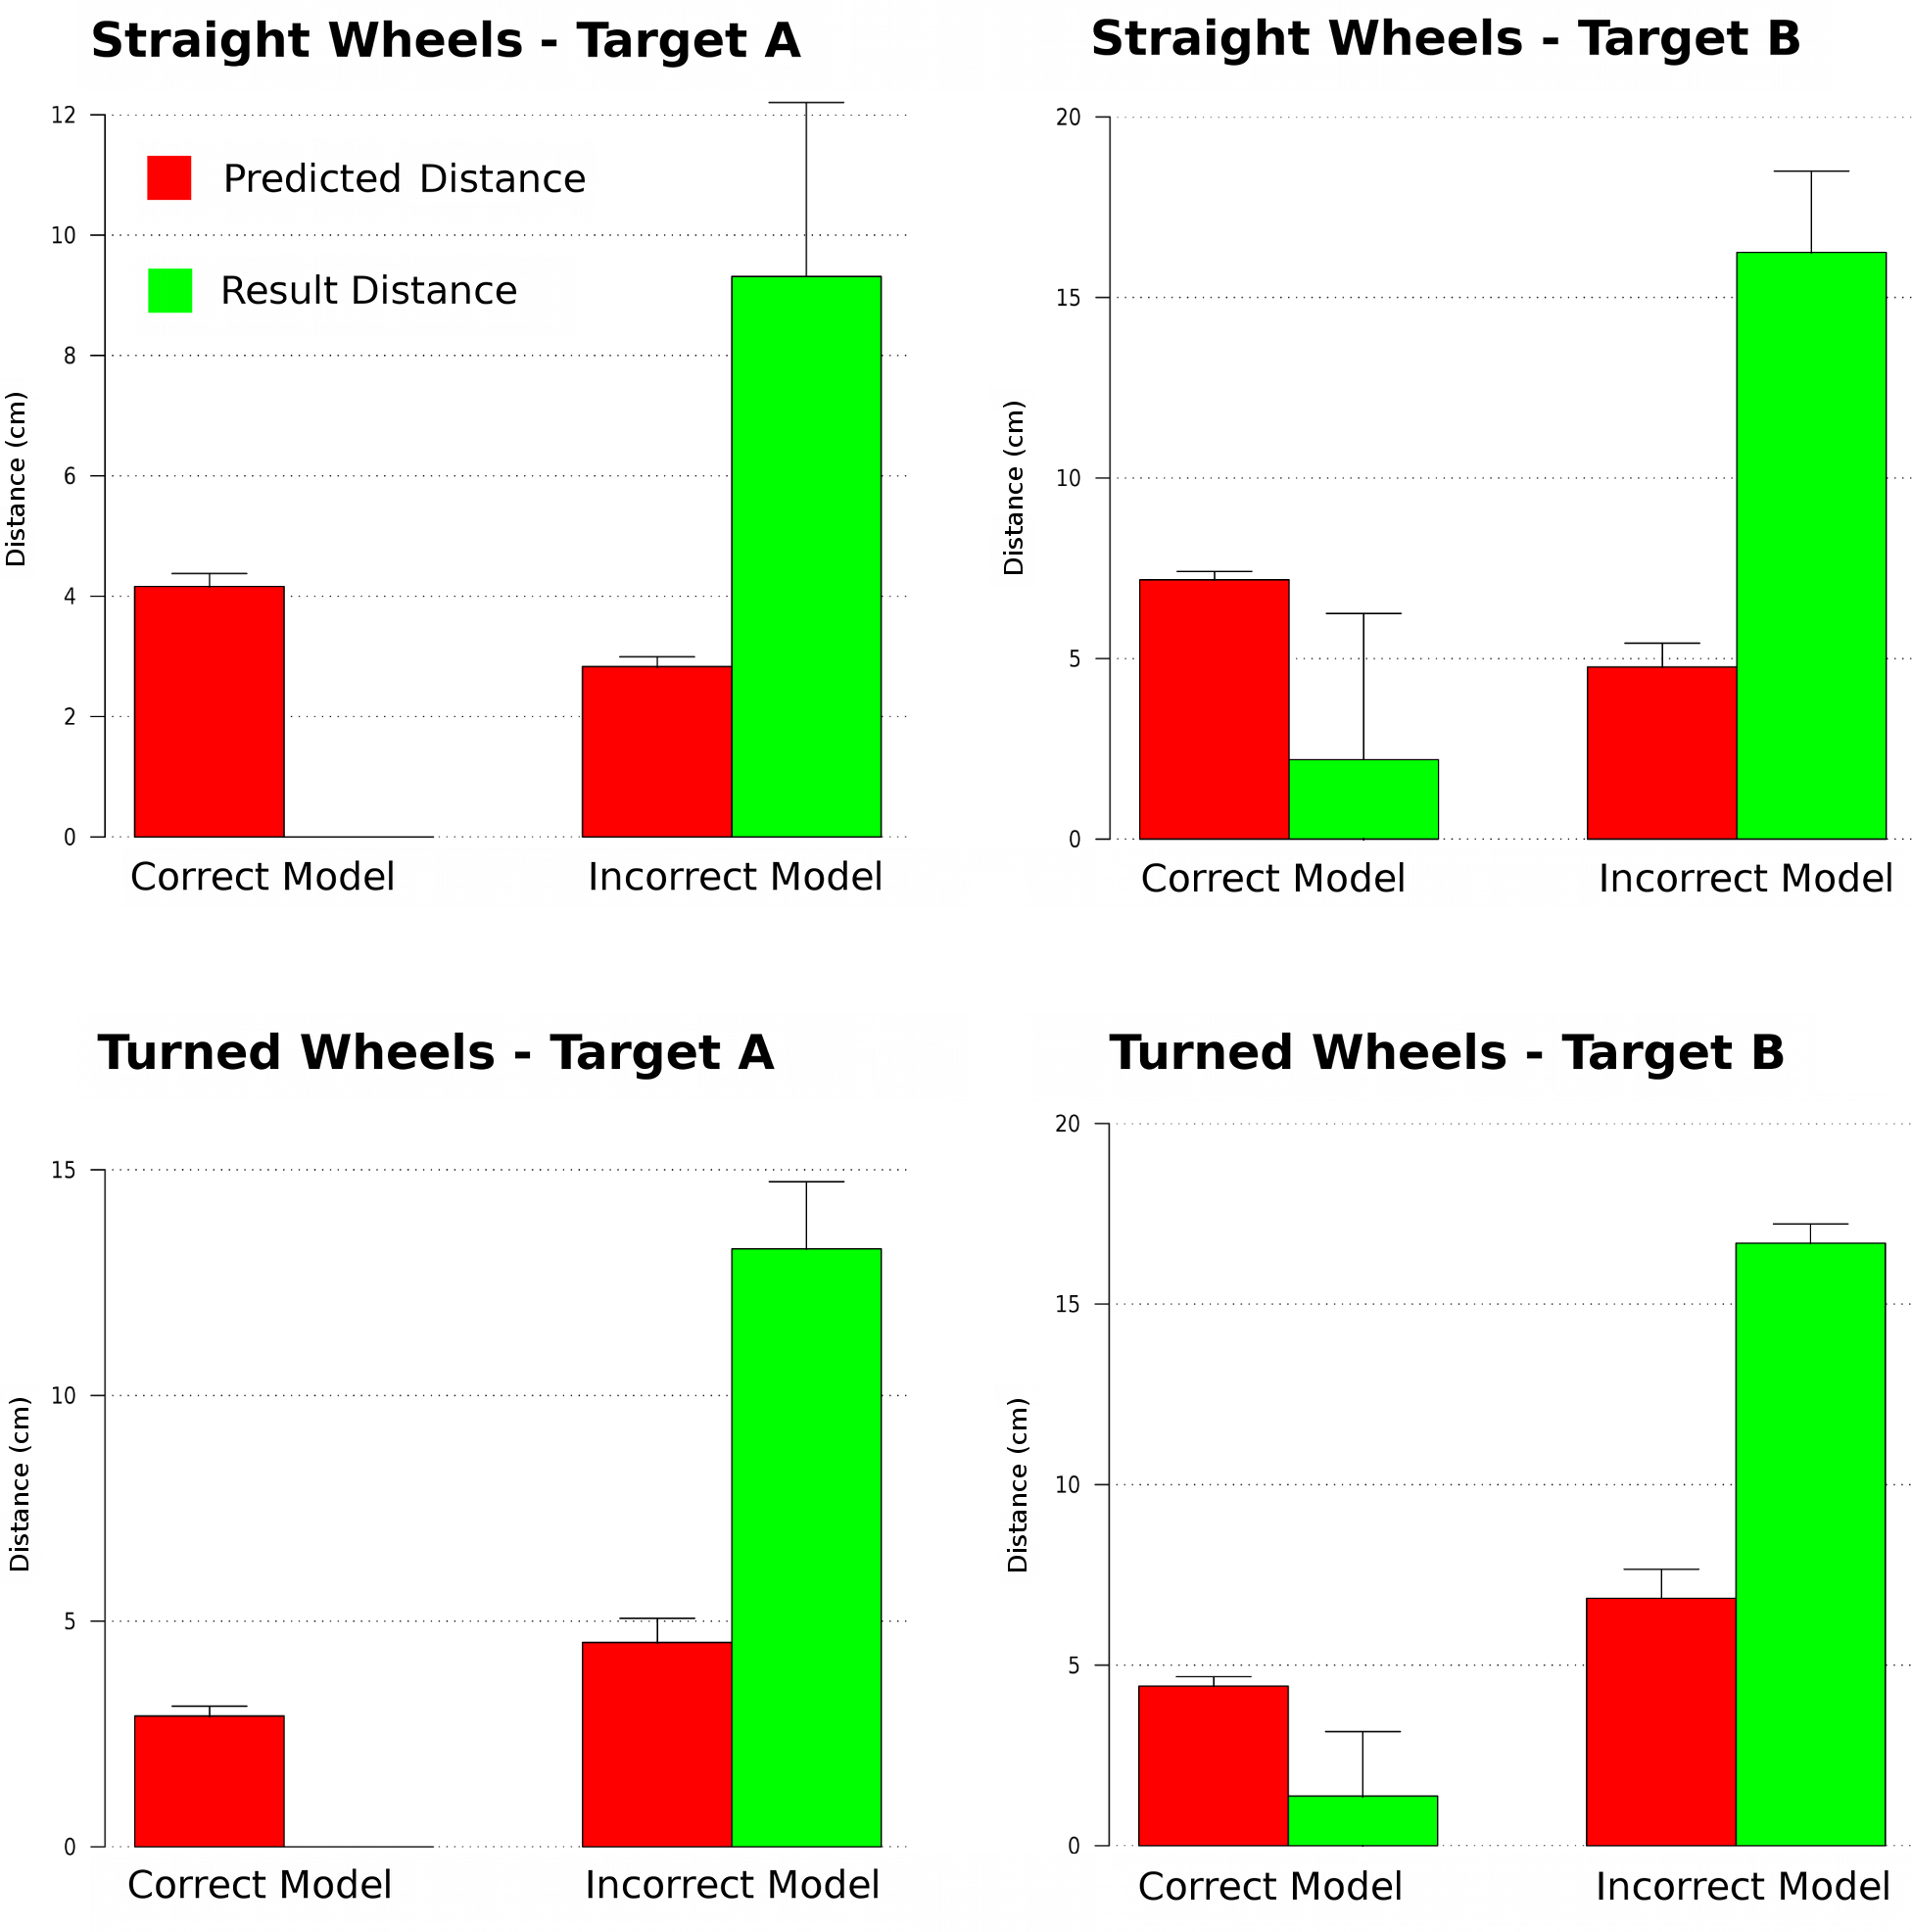
\includegraphics[width=1\textwidth]{images/knock}
\par\end{centering}

\caption{Predicted and actual results of using a box-cart to knock down an
out of reach cylinder, expressed as a distance between the box-cart
and the target cylinder. The predicted results are the value of the
objective function used to determine the best cart release pose. This
is computed from the simulated distance between the box-cart centre
and the cylinder position. The result distance is the smallest distance
between the cylinder and the box-cart after it comes to rest. The
errors bars represent the standard deviation across eight repeated
iterations of each scenario.\label{fig:Knock-tool-use}}


\end{figure}


These results clearly demonstrate the importance of learning the correct
object physics model, which allows accurate prediction of action outcomes
and task planning. When the robot had an incorrect model of the object
it was unable to successfully complete the task even once. It should
be noted that when the cylinder is in position B, the lower success
rate is due to the longer distance between the cylinder and the end
of the ramp. The further the distance the larger the drift of the
box-cart trajectory, which results from positioning errors, and small
variations in the table and ramp surface, as well as the wheel axles.


\section{Discussion\label{sec:Discussion-1}}

In this chapter we have presented a general method for a robot to
determine hidden properties of an object by building a predictive
model of the object using experimentation and simulation. A simulator
is used to calculate the outcome probabilities of various actions
that the robot can perform on an object, as well as to determine which
is the most informative given a hypothesis distribution. The expected
KL divergence is used to deterine the information gain of an action.
By choosing the most informative action, the robot can learn the model
of the object in a minimum number of iterations, minimising wear and
tear as well as time taken.

We have presented both a generalised algorithm as well as several
concrete implementations of the system. We have demonstrated the robot
determining the centre of mass of a box and cylinder by dropping the
object and using the resulting pose to gain information as to the
location of the centre of mass. We have demonstrated the robot determining
the wheel configuration of a box-cart by releasing it from an angled
ramp, and by looking at where it comes to rest the robot can determine
the orientation of the wheels and whether they are free to rotate.
We have demonstrated the generality of our method by using it to model
the behaviour of another robot responding to outside stimuli. Finally,
we showed a simple tool use task in which the robot uses a learned
model of an object in order to plan and complete a goal. The robot
uses a predictive physics engine model of a box-cart object to determine
the optimal pose to release it from on an angled ramp in order to
knock down a cylinder located some distance from the ramp.

It must be noted that some of the results of the concrete system implementations
showed a higher than expected variance in terms of the robot's confidence
distribution over the potential object models. This is almost certainlty
due to the greatly simplified noise model used during action simulation,
as compared to the real world noise model. When building the action
probability models we typically used a simple linear Gaussian noise
model. However, in the real world the noise would in many instances
be highly non-linear and non-Gaussian. For example, one of the most
common error modes during the \emph{Centre of Mass Experiment} was
for the robot to place the object too low, resulting in the bottom
of the object striking the table surface. This would in turn shift
the object in the gripper, changing its orientation greatly. This
type of noise is not accounted for during simulation and would require
a more detailed simulation, including simulating the robot arm and
its grasp of the object. We leave this for future work.


\section{Future Work\label{sec:Future-Work-1}}

The work presented in this chapter sets out a general framework for
determining an object's model, which can then be used for further
task planning and prediction. However, there are several unresolved
issues which should be addressed in future work.

First, the presented approach is limited to classifying a given object
into one of several pre-determined models. These models are discrete,
finite, and fixed. However, many of the properties which determine
the nature of an object are inherently continuous values. For example,
the coefficient of friction of a surface, or the location of the centre
of gravity. We may discretise the values as an approximation, but
this may result in a very large number of potential models, which
would in turn result in a large computational load to simulate all
of the actions on all of the models. Instead, it may be possible to
adapt the presented method to perform an optimisation search through
the continuous parameter space to determine the most accurate object
model.

Likewise, the set of possible actions that the robot can perform is
predetermined and fixed. A possible improvement is to allow the robot
to dynamically add new actions to choose from. It may be able to use
information about the quality of existing actions to generate new
instances of increased quality, while rejecting ones with a low expected
information gain. This may be increasingly important for action models
with a large parameter space. The models we used in the previous examples
were of low dimensionality, described by only 2 or 3 parameters. However,
for more complicated models with many parameters, providing sufficient
coverage of the parameter space may not be feasible with a fixed predetermined
set of actions. Rather the robot would need to dynamically search
through the parameter space.

Third, the result space of each action is restricted to being finite
and discrete in the form of a fixed number of result labels. This
is essentially a method of function approximation of the underlying
probability distribution over the resulting world state after an action
is performed. The discrete and finite nature of the function approximation
simplifies the update of the confidence over the potential models
distribution, as well as simplifying the calculation of the expected
information gain. However, using discretisation as a function approximation
leads to a potential loss of information. A future improvement could
be to move to some form of sampling method for representing the probability
distribution over the result world states. 

Finally, we have only demonstrated a very simple planning and tool
use task using the learned object model in Section \ref{sec:Learned-Model-Exploitation}.
In this task the action performed by the robot was predetermined ahead
of time, the only planning involved was to determine the parameters
for the action (where to release the box-cart). This is sufficient
to demonstrate the predictive qualities of the learned model, but
for more complex tasks and actions a more comprehensive planner should
be used. Additionally, a potential future direction is to use the
learned quantitative model of the object to learn a higher leavel
qualitative model, which would improve model generalisation and planning
of complex actions.
\end{document}
